% INFORMAÇÃO SOBRE A VERSÃO DESSE DOCUMENTO
% VERSÃO DA CLASSE ppgccufmg 1.44 (de 2011-04-25) - http://vilarneto.com/ppgccufmg
% VERSÃO ORIGINAL: http://www.dcc.ufmg.br/pos/alunos/modelodisstese.php
% VERSÃO COMENTADA e EXEMPLIFICADA: http://www.dcc.ufmg.br/~mirella @ janeiro/2012

\documentclass[msc]{ppgccufmg}  % [phd] se for doutorado
                                % [phd,project] para proposta de tese 
                                % [msc] se for mestrado

\usepackage[brazil]{babel}      % se o documento for em português, OU
%\usepackage[english]{babel}    % se o documento for em inglês
\usepackage[utf8]{inputenc}   % Dá suporte para caracteres especiais como acentos e cedilha
\usepackage[T1]{fontenc}        % Lê a codificação de fonte T1 (font encoding default é 0T1).
\usepackage{type1ec}
\usepackage{graphicx}           % define o comando \includegraphics para a inclusão de figuras
\usepackage[a4paper,
  portuguese,
  bookmarks=true,
  bookmarksnumbered=true,
  linktocpage,
  colorlinks,
  citecolor=black,
  urlcolor=black,
  linkcolor=black,
  filecolor=black,
  ]{hyperref}
\usepackage[square]{natbib}    % permite citações naturalmente
                               % integradas ao texto
\usepackage{multirow}					 % permite fazer tabelas com múltiplas linhas
\usepackage{amstext}

% \makeatletter
% \let\c@lofdepth\relax
% \let\c@lotdepth\relax
% \makeatother
\usepackage[caption=false]{subfig}
% \usepackage{subfig}
% \usepackage{float}
\usepackage[compatibility=false]{caption}
\usepackage{amsmath}
\usepackage{morefloats}

% \hyphenation{re-qui-si-to, com-ple-xi-da-de} % para separar corretamente
\hyphenation{a-na-li-san-do
	     a-pre-sen-ta-mos
	     a-pro-pri-a-da
	     de-fi-ni-mos
	     di-fe-ren-te
	     ca-rac-te-ri-za-dos
	     co-la-bo-ra-ção
	     co-la-bo-ra-ções
	     com-ple-xi-da-de
	     con-fe-rên-cia
	     con-fe-rên-cias
	     cons-tru-ir
	     con-si-de-ra-vel-men-te
	     fi-gu-ras
	     ge-ra-ção
	     hi-e-rár-qui-co
	     i-te-ra-ção
	     in-te-res-sa-dos
	     mí-ni-mo
	     mo-de-lo
	     mo-de-la-gem
	     pro-ble-ma
	     per-cen-ta-gem
	     pu-bli-ca-ção
	     pu-bli-ca-ções
	     pu-bli-ca-ram
	     re-a-li-za-das
	     re-a-li-za-mos
	     re-pre-sen-ta-das
	     re-qui-si-to 
	     res-pon-sá-veis
	     se-me-lhan-tes
	     si-mi-la-res
	     sig-metrics
	     so-ci-ais
	     su-per-li-ne-ar
	     va-lo-res
	     va-ria-mos
	     } % para separar corretamente    

\usepackage[usenames,dvipsnames]{xcolor}  % para poder usar os nomes das cores
%cria um novo comando para comentários em vermelho no meio do texto
\newcommand{\redcomment}[1]{\textcolor{red}{\textbf{\textit{#1}}}} %M


\begin{document}

% O comando a seguir, \ppgccufmg, provê todas as informações relevantes para a
% classe ppgccufmg. Por favor, consulte a documentação para a descrição de
% cada chave.

% Um exemplo para documentos em portuguÊs é apresentado a seguir:
\ppgccufmg{
  title={Um Estudo sobre a Evolução Temporal de Comunidades Científicas},
  authorrev={Alves, Bruno Leite},
  cutter={A474e}, % INFORMAÇÃO QUE VAI NA FICHA CATALOGRÁFICA
  cdu={519.6*62(043)},  % Define o identificador CDU do documento, fornecido pela Secretaria do Curso.
  university={Universidade Federal de Minas Gerais - Departamento de Ciência da Computação},
  course={Ciência da Computação},
  address={Belo Horizonte},
  date={2013-08}, % ANO-MÊS  DA DEFESA
%   keywords={Comunidades Científicas, Núcleos de Comunidades, Evolução de Comunidades}, %Define as palavras-chave que deverão constar na Ficha Catalográfica,
  keywords={Computação - Teses, Redes de Relações Sociais - Teses, Instituições e Sociedades Científicas – Teses, Teoria dos Grafos - Teses, Redes Complexas - Teses}, %Define as palavras-chave que deverão constar na Ficha Catalográfica,
  postkeywords={Orientador, Coorientador, Título},
%   separadas por vírgulas.
  advisor={Alberto Henrique Frade Laender},
  coadvisor={Fabrício Benevenuto de Souza},
%  approval={img/approvalsheet.eps},
  abstract=[brazil]{Resumo}{resumo}, %resumo.tex
  abstract=[english]{Abstract}{abstract}, %abstract.tex
%   abstract=[brazil]{Resumo Estendido}{resumoest}, %resumoest.tex
  dedication={dedicatoria},
  ack={agradecimentos},
%  ack=[Acknowledgments]{ack},
%   epigraphtext={\redcomment{Uma jornada de mil milhas começa com um único passo.}}{Lao-Tzu},
  epigraphtext={De tudo, ficaram três coisas: a certeza de que ele estava sempre começando, a certeza de que era preciso continuar e a certeza de que seria interrompido antes de terminar. Fazer da interrupção um caminho novo. Fazer da queda um passo de dança, do medo uma escada, do sono uma ponte, da procura um encontro.}{Fernando Sabino},
  approval={folha_aprovacao.eps},
 }
 %OUTRAS SUGESTÕES DE EPIGRAPH:
  %{Escolhe um trabalho de que gostes \\e não terás que trabalhar nem um dia na tua vida.}{Confúcio}
  %{O único modo de escapar da corrupção causada pelo sucesso é continuar trabalhando.}{Albert Einstein},
  %{Que ninguém se engane, só se consegue a simplicidade através de muito trabalho.}{Clarice Lispector},
  %{Um sonho sonhado sozinho é um sonho. Um sonho sonhado junto é realidade.}{Raul Seixas},
  %{Para o trabalho que gostamos levantamo-nos cedo e fazemo-lo com alegria.}{William Shakespeare},
  %{Pensar é o trabalho mais difícil que existe. Talvez por isso tão poucos se dediquem a ele.}{Henry Ford},
  %{O prazer no trabalho aperfeiçoa a obra.}{Aristóteles},
  %{O caminho batido não leva a novas pastagens}{Indira Ghandi},
  %{Uma jornada de mil milhas começa com um único passo.}{Lao-Tzu},
  %{É sempre o aventuroso que consegue grandes coisas}{Montesquieu},
%  De tudo, ficaram três coisas: a certeza de que ele estava sempre começando, a certeza de que era preciso continuar e a certeza de que seria interrompido antes de terminar. Fazer da interrupção um caminho novo. Fazer da queda um passo de dança, do medo uma escada, do sono uma ponte, da procura um encontro. {Fernando Sabino}

% VOCÊ PODE DIVIDIR O SEU TEXTO EM VÁRIOS ARQUIVOS, por exemplo, um para cada seção principal do seu trabalho: introducao.tex, relacionados.tex, metodologia.tex, experimentos.tex, conclusao.tex
%%%%%%%%%%%%%%%%%%%%%%%%%%%%%%%%%%%
\chapter{Introdução}\label{introducao}
%%%%%%%%%%%%%%%%%%%%%%%%%%%%%%%%%%%

%%%%%%%%%%%%%%%%%%%%%%%%%%%%%%%%%%%
\section{Motivação}
%%%%%%%%%%%%%%%%%%%%%%%%%%%%%%%%%%%
% \redcomment{Revisar tradução e texto. Adicionar mais trabalhos e detalhar melhor alguns.}

Desde os seus primórdios, a sociedade tem se organizado em comunidades, ou seja, grupos de indivíduos 
com interesses em comum\footnote{http://www.merriam-webster.com/dictionary/community}. Particularmente, 
a proliferação de novas tecnologias de comunicação baseadas na Internet tem facilitado a rápida 
formação e crescimento de comunidades \textit{online}~\citep{Kleinberg2008}. Comunidades possuem uma grande 
quantidade de características e servem a vários propósitos. Elas podem ser desde pequenos 
grupos hermeticamente comprometidos com temas específicos, como comunidades científicas de determinadas áreas, 
até mesmo grupos de milhões de usuários ligados por um interesse em comum, tais como comunidades 
relacionadas a esporte ou fãs de uma celebridade.
% Since its beginning, society has been organizing itself into communities, which are groups of individuals with common interests\footnote{http://www.merriam-webster.com/dictionary/community}.
% Particularly, the proliferation of new communication technologies based on the Internet has facilitated the rapid formation and growth of on-line communities~\cite{Kleinberg@cacm2008}. 
% Communities exhibit a wide range of characteristics and serve a variety of purposes, from small groups engaged in tightly niche topics such as a very specific scientific community, 
% to millions of users linked by an interest such as a community related to a sport team or fans of a celebrity. 

Geralmente, indivíduos que são socialmente conectados em comunidades tendem a compartilhar interesses comuns
e outras similaridades. Embora existam muitos fatores que possam determinar a formação de uma comunidade
e o seu crescimento, existem duas forças que explicam a formação de comunidades: influência 
e homofilia. Por um lado, influência postula que indivíduos mudam para se tornarem mais similares
a seus amigos na comunidade. Por outro lado, homofilia postula que indivíduos criam conexões 
sociais dentro de uma comunidade justamente porque já são similares. Esforços recentes 
têm mostrado evidências quantitativas que ambas as forças~\citep{Cha2010,Backstrom2006},
teorias~\citep{Rogers1962,Watts2007} e modelos existentes~\citep{Kempe2003,Kempe2005} 
dependem da identificação de um grupo influente 
de indivíduos com o poder de afetar não somente a estrutura topológica de uma comunidade, 
mas também interferir na difusão e no fluxo de informação da comunidade.
% Often, individuals who are socially connected in a community tend to share interests and similarities. Although, there are many factors that might determine a community formation
% and its growth, there are two main driven forces used to explain similarity in a community formation: influence and homophily. On one hand, influence posits that individuals change
% to become more similar to their friends in the community. On the other hand, homophily postulates that individuals create social connections within a community precisely because
% they are already similar. Recent efforts have provided quantitative evidences of both forces~\cite{icwsm10cha,crandall.kdd08,Backstrom:2006,influence.correlation.kdd08} and
% existing theories~\cite{Rogers.1962,accidental-influential}, models~\cite{kempe03kdd,Kempe05influentialnodes}, and
% approaches~\cite{saez-trumper@kdd12,Weng:2010:TFT:1718487.1718520} rely on identifying a group of influential individuals with the power to affect not only the underlying network
% structure of a community, but also to interfere on the spread and flow of information within a community. 

Nesta dissertação, apresentamos uma perspectiva diferente e um estudo complementar desse problema. 
Aqui, nos concentramos em estudar os papéis que indivíduos influentes em comunidades científicas
desempenham na evolução das propriedades de tais comunidades. Intuitivamente, quando pesquisadores 
importantes e com grande influência em suas áreas decidem se juntar ou deixar uma comunidade científica, levam com eles recursos,
experiência e até mesmo estudantes, e possivelmente influenciam outros membros a fazerem o mesmo. Para esse 
estudo, usamos dados da DBLP\footnote{http://dblp.uni-trier.de/} para construir 
comunidades científicas, representadas pelas principais conferências
dos SIGs\footnote{http://www.acm.org/sigs} (\textit{Special Interest Groups}) da ACM\footnote{http://www.acm.org}
(\textit{Association for Computing Machinery}). Então, propomos uma estratégia para definir o 
núcleo de uma dada comunidade científica, juntamente com seus líderes em um dado período de 
tempo. Finalmente, investigamos como os aspectos do núcleo impactam a estrutura topológica da comunidade.

% In this paper, we take a different perspective and study a complementary problem. Here, we focus on studying the roles that influential individuals from a scientific community play
% on evolving properties of such communities. Intuitively, when prolific research leaders decide to join or leave a community, they take with them resources,
% experience and students, and possibly influence other members to do the same. For this study, we use data from DBLP to construct scientific communities, represented by the 
% main ACM SIG conferences. Then, we propose a strategy to infer the community core, the leaders of a given scientific community in a given period of time. 
% Finally, we investigate how aspects of the core impact on the community underlying structure. 

O estudo do núcleo de comunidades científicas pode ser visto de duas perspectivas diferentes. A 
primeira é a sociológica, vindo da necessidade de compreender como partes da sociedade evoluem, 
bem como responder a perguntas de longa data relacionadas com à interação entre os diferentes 
tipos de participante. Em contrapartida, sob uma perspectiva tecnológica, compreender estes 
aspectos é crítico para muitas aplicações relacionadas a predição de \textit{links}~\citep{Getoor2005}. Tal estudo, entretanto, 
tem sido difícil devido à caracterização de alguns conceitos, como conexões humanas e uma definição apropriada 
de liderança, sendo difícil até mesmo de se reproduzir em grande escala dentro de um laboratório de pesquisa.
% The study of the core of scientific communities is of interest from two different perspectives.  The first is sociological, coming from the necessity to understand how
% segments of society evolve as well as to answer longstanding  questions related to the interaction among different types of participant. On the other hand, from a technological perspective,
% understanding these aspects is critical for several applications related to link prediction. Such a study, however, has been difficult as essential components like human connections 
% and a proper definition of leadership is hard to be reproduced at a large scale within the confines of a research laboratory.

%%%%%%%%%%%%%%%%%%%%%%%%%%%%%%%%%%%
%%%%%%%%%%%%%%%%%%%%%%%%%%%%%%%%%%%
\section{Trabalhos Relacionados}
%%%%%%%%%%%%%%%%%%%%%%%%%%%%%%%%%%%
% \redcomment{Revisar tradução e texto. Adicionar mais trabalhos e detalhar melhor alguns.}

Recentemente, esforços tem sido feitos com o intuito de analisar a estrutura das comunidades e a evolução de suas redes.
Particularmente, \cite{Kumar2006} analisaram duas grandes redes através do tempo, Flickr\footnote{http://www.flickr.com/} e Yahoo! 360, para encontrar uma 
segmentação dessas redes em indivíduos isolados, componentes intermediários, que também são comunidades isoladas, e o maior 
componente conectado. Nesse trabalho, os autores identificaram que alguns componentes possuem um centro constituído 
de nodos de maior grau com muitos nodos de menor grau conectados a eles e que foram caracterizados 
estrelas, isto é, componentes que são formados rapidamente, mas não são absorvidos pelo maior componente conectado.
Assim, eles propuseram um modelo de crescimento capaz de gerar redes com características similares às das redes estudadas.
Este modelo se baseia em três tipos de nodo: passivos, recrutadores e agregadores. Usuários passivos se juntam à rede pela
curiosidade ou pela insistência de amigos, mas nunca se comprometem efetivamente em atividades da rede. Recrutadores estão
interessados em transformar comunidades \textit{offline} em comunidades \textit{online} e recrutar seus amigos a participarem 
da rede. Por fim, os agregadores são participantes que contribuem ativamente para o crescimento da rede e frequentemente se conectam a outros 
membros semelhantes.

\cite{Ducheneaut2007} extraíram e caracterizaram explicitamente, comunidades criadas a partir de cinco servidores do 
\textit{World of Warcraft}, um jogo multijogador massivo. O estudo é centralizado em grupos de jogadores 
formados para realizar atividades em conjunto, denominados guildas. Tais grupos apresentam dificuldades 
consideráveis de administração e muitos não sobrevivem ao longo do tempo, sendo os líderes membros importantes para a 
longevidades das guildas. Os autores apresentaram algumas propriedades demográficas sobre esses grupos, 
tais como, distribuição do tamanho das guildas, interação de membros e não membros de guildas em eventos 
do jogo, e tamanho das guildas ao longo do tempo. Em seguida, mostraram o impacto das guildas na estrutura da 
rede utilizando métricas clássicas de redes complexas como centralidade e densidade. Eles sugeriram ainda
um painel para monitorar o tamanho, número de subgrupos e densidade das guildas, além de uma visualização da topologia 
da rede.

Complementarmente ao estudo de \cite{Ducheneaut2007}, \cite{Patil2012} analisaram e modelaram fatos que levam usuários a deixar 
ou entrar em guildas do jogo \textit{World of Warcraft}. Nesse trabalho os autores propõem um modelo capaz de predizer se e 
quando um jogador irá deixar a comunidade e também qual o impacto dessa saída. Este modelo é baseado em 
várias características, tais como, níveis dos jogadores e das guildas, atividades do jogo e características sociais. Estas 
características sociais estão ligadas a um jogador podendo ser o seu número de amigos, o número de amigos que já deixaram a comunidade, 
e a percentagem de membros na comunidade que interagem com o jogador em questão, bem como a frequência. O modelo construído se mostrou
efetivo em predizer quando os usuários deixarão suas comunidades e quando essas comunidades irão se desfazer na rede.

\cite{Viswanath2009} estudaram dois tipos de rede formados a partir de dados do Facebook\footnote{http://www.facebook.com}. A primeira rede foi construída utilizando 
os laços de amizade entre os usuários e a segunda utilizando as interações entre os usuários, e.g., postagens em mural e seus 
comentários. Eles constataram que muitos usuários aceitam pedidos de amizade por cortesia, de modo que a rede baseada
em laços de amizades apresenta um crescimento surreal. A rede construída a partir das interações entre os usuários possui comportamento 
diferente. Nessa rede, os laços tendem a surgir e desaparecer rapidamente através do tempo, e a força dos laços apresenta, de forma geral, 
uma tendência decrescente das atividades que acompanham a idade dos \textit{links} nas redes sociais. O trabalho também apresenta a métrica 
\textit{resemblance}, utilizada para medir a sobreposição entre duas instâncias da rede, para mostrar que a rede possui um núcleo que
persiste através do tempo. Finalmente, os autores apresentam uma análise utilizando métricas clássicas de redes complexas, mostrando
que as propriedades estruturais das redes estudadas não apresentam grandes variações ao longo do tempo.

% Recentemente, esforços tem sido feitos com o intuito de analisar a estrutura das comunidades e a evolução de suas redes. 
% Particularmente, \cite{Kumar2006} analisaram duas grandes redes para encontrar uma segmentação dessas redes
% em indivíduos isolados, comunidades isoladas e o maior componente conectado. Assim, eles propuseram um modelo de crescimento das
% redes apto a gerar redes com características similares a das redes estudadas. \cite{Ducheneaut2007} extraíram e caracterizaram 
% explicitamente, comunidades criadas a partir de \textit{World of Warcraft}, um jogo multijogador massivo.
% Complementarmente, \cite{Patil2012} analisaram e modelaram fatos que levam usuário a deixarem ou entrarem
% em comunidades de jogos online. \cite{Viswanath2009} estudaram a evolução das atividades entre 
% usuário no Facebook e encontraram que alguns links em atividades na rede tendem a surgir e desaparecer rapidamente através do tempo, e
% a força dos laços apresentam, de forma geral, uma tendência decrescente das atividades que acompanham as idades dos links nas 
% redes sociais.
% There has been a number of recent efforts that attempt to analyze community structure and network evolution.  Particularly, Kumar \textit{et al.}~\cite{Kumar:2006} analyzed two large networks to
% find a segmentation of these networks into singletons, isolated communities, a giant component. Then, they propose a network growth model able to generate networks with similar
% characteristics.  Ducheneaut \textit{et al.}~\cite{Ducheneaut:2007} extracted and characterized explicitly created communities from the World of Warcraft, a massive multiplayer game.
% Complementarily, Patil \textit{et al.}~\cite{Patil:2012} analyzed and modeled factors that make users to leave or join on-line gaming communities.  Viswanath \textit{et
% al.}~\cite{Viswanath:2009} studied the evolution of activity between users in Facebook and found that that links in the activity network tend to come and go rapidly over time, and
% the strength of ties exhibits a general decreasing trend of activity as the social network link ages.

Em termos de modelos para redes sociais dinâmicas, \cite{Leskovec2005} investigaram nove redes, que incluem redes de citações de 
diferentes áreas da física, citações de patentes americanas e afiliações de pesquisadores, para mostrar 
que essas redes densificam ao longo do tempo, com o número de arestas crescendo de forma superlinear em relação
ao número de nodos e que o caminho mínimo médio entre os nodos geralmente diminui através do tempo. Baseado nessas observações, eles 
desenvolveram um modelo de geração de redes que incorpora tais propriedades, chamado de \textit{Forest Fire}. Esse modelo necessita
apenas de dois parâmetros e é capaz de capturar padrões como a lei de potência da densificação e redução do diâmetro. Mais recentemente, 
\cite{Leskovec2008} apresentaram um estudo detalhado da evolução de redes por meio da análise de quatro grandes 
redes sociais \textit{online}, são elas: Flickr, Delicious\footnote{http://delicious.com/}, 
Answers\footnote{http://www.answers.com/} e LinkedIn\footnote{http://www.linkedin.com}. Eles investigaram uma grande variedade de estratégias de formação 
de redes para mostrar que a localização das arestas desempenha um papel crítico na evolução dessas redes. Baseados nessas observações, 
os autores desenvolveram um modelo de evolução em que novos nodos surgem na rede com uma taxa predeterminada. O modelo também 
considera que novas arestas possuem distâncias muito curtas, normalmente formando triângulos, sendo assim, o modelo segue este padrão para 
formação de novas arestas. Diferentemente dos esforços acima referidos, nosso trabalho foca em propriedades das comunidades e no papel que 
os líderes dessas comunidades desempenham na topologia da rede.

% Em termos de modelos para redes sociais dinâmicas, \cite{Leskovec2005} investigaram uma grande número 
% de grafos para mostrar que grafos densificam ao longo do tempo, com o número de arestas crescendo de forma superlinear em relação
% ao número de nodos e a distância média entre os nodos geralmente diminuem através do tempo. Baseado nessas observações, eles 
% desenvolveram um modelo de geração de grafos que incorpora tais propriedades. Mais recentemente, \cite{Leskovec2008} 
% apresentaram um estudo detalhado de evoluções de redes pela análise de quatro grandes redes sociais online. Eles investigaram uma grande
% variedade de estratégias de formações de redes para mostrar que a localização das arestas desempenham um papel crítico na evolução das redes.
% Baseado nessas observações, eles desenvolveram um modelo de evolução de redes, em que nodos alcançam uma taxa predeterminada. Diferentemente
% dos esforços acima referidos, nosso trabalhos foca em propriedades das comunidades e no papel que os líderes das comunidades desempenham
% na topologia da rede.
% In terms of models for network dynamics, Leskovec \textit{et al.}~\cite{Leskovec:2005} investigated a wide range of real graphs to show that graphs densify over time, with the
% number of edges growing super linearly in the number of nodes and that the average distance between nodes often shrinks over time. Based on these observations, they develop a graph
% generation model that incorporates such properties.  More recently, Leskovec \textit{et al.}~\cite{Leskovec:2008} presented a detailed study of network evolution by analyzing four
% large on-line social networks.  They investigated a wide variety of network formation strategies to show that edge locality plays a critical role in the evolution of networks. Based on
% this observation, they developed a model of network evolution, in which nodes arrive at a pre-specified rate.  Differently from the above efforts, our work focuses on community
% properties and the roles that community leaders play in the underlying network structure.

Alguns outros trabalhos também abordaram o estudo de comunidades científicas. Particularmente, \cite{Backstrom2006} 
estudaram comunidades na LiveJournal\footnote{http://www.livejournal.com/} e comunidades científicas extraídas 
da DBLP. Esses dois conjuntos de dados possuem comunidades explícitas, onde 
conferências representam comunidades na DBLP. Os autores identificaram que as tendências que levam 
indivíduos a entrar em comunidades e comunidades a crescer rapidamente dependem sutilmente da topologia 
da rede. Por exemplo, a tendência de um indivíduo a entrar em uma comunidade é influenciada não só pelo número 
de amigos que ele possui dentro daquela comunidade, mas também de como esses amigos estão conectados entre si. Eles utilizaram 
técnicas de árvore de decisão para identificar as estruturas mais significativas que afetam estas comunidades, 
e desenvolveram uma nova metodologia capaz de mensurar a mudança de indivíduos entre comunidades 
e também verificar como isto está relacionado com mudanças de interesse dentro das comunidades.

\cite{Huang2008} usaram os dados da biblioteca digital CiteSeer\footnote{http://citeseer.ist.psu.edu} 
para construir uma rede de coautoria em Ciência da Computação abrangendo pesquisas realizadas entre 1980 e 
2005. Eles realizaram estudos sobre tendências de evolução das colaborações sob duas perspectivas, rede completa 
e comunidades. Entre as suas principais observações, eles mostraram que a área de Ciência da Computação apresenta 
padrões de colaboração mais similares à Matemática do que à Biologia. Além disso, eles também quantificaram 
e compararam padrões de colaboração de seis comunidades dentro da área da Ciência da Computação: 
Inteligência Artificial, Aplicações, Arquitetura, Bancos de Dados, Sistemas e Teoria. Com base nessas 
informações, os autores propuseram um modelo de aprendizagem e predição de colaborações entre pares de autores.
Diferente desses esforços, nesta dissertação focamos no estudo das propriedades do núcleo da comunidade, de modo que 
nossas análises são complementares a essas.

% Existem também esforços que tentaram estudar comunidades científicas. Particularmente, \cite{Backstrom2006} 
% estudaram comunidades na LiveJournal~\footnote{http://www.livejournal.com/} e comunidades científicas extraídas da DBLP~\footnote{http://dblp.uni-trier.de/} 
% para encontrar que a tendência dos indivíduos entrarem nas comunidades e das comunidades de crescerem rapidamente, depende sutilmente da topologia da rede. 
% \cite{Huang2008} usaram os dados da DBLP para construir a rede do campo de Ciência da Computação cobrindo a colaboração de pesquisa de 1980 a 2005. Entre
% as suas principais observações, eles mostraram que o campo de Ciência da Computação apresentam o padrão de colaboração mais similar para 
% a Matemática do que para a Biologia. Diferente desses esforços, aqui nós focamos no estudo das propriedades do núcleo da comunidade, assim, 
% nossas análises são complementares a essas.
% There are also efforts that attempted to study scientific communities. Particularly, Backstrom \textit{et al.}\cite{Backstrom:2006} studied communities in LiveJournal and
% scientific communities extracted from DBLP to find that the propensity of individuals to join communities and of communities to grow rapidly, depends in subtle ways on the
% underlying network structure. Huang \textit{et al.}~\cite{Huang:2008} used DBLP data to construct a network for the Computer Science field covering research collaborations from
% 1980 to 2005. Among their main observations, they show that the Computer Science field presents a collaboration pattern more similar to Mathematics than to Biology.  
% Different from these efforts, here we focus on studying the properties of the community core, thus, our analyses are complementary to
% theirs.

Quando se trata de identificar núcleos de comunidades, existem várias abordagens que extraem 
o núcleo tendo como base as propriedades topológicas da rede. \cite{Leskovec2010} compararam vários algoritmos 
de detecção de comunidades em vários tipos de rede. Neste trabalho, uma comunidade é definida como nodos que possuem mais ligações
entre si do que com o restante da rede. Os autores apontam que, de forma geral, os algoritmos são otimizados e 
detectam as comunidades efetivamente. No entanto, existem classes de redes em que os algoritmos executam de 
forma subótima. Já \cite{Chakrabarti2006} propuseram um arcabouço baseado em agrupamento hierárquico 
aglomerativo e \textit{k-means} para realizar o agrupamento de dados através do tempo. Eles consideraram dois critérios para avaliação: 
(i) o agrupamento ao longo do tempo não deve apresentar grandes diferenças em relação aos dados globais e 
(ii) o agrupamento não deve mudar drasticamente de uma iteração para outra. Eles construíram uma rede 
a partir de dados do Flickr e constaram que o arcabouço proposto atende aos dois critérios definidos. 
\cite{Hopcroft2004} também propuseram um arcabouço baseado em 
agrupamento hierárquico capaz de identificar comunidades na biblioteca digital CiteSeer. Além dessas comunidades,
eles também apontaram um grupo de artigos que aparece várias vezes nos grupos identificados ao longo do 
tempo, dos quais eles denominaram como núcleo da rede. Tais abordagens não são aplicáveis em nosso 
contexto, já que estamos interessados no estudo das propriedades dos núcleos.

% \cite{Sachan2012}
% ~\citep{Leskovec2010,Chakrabarti2006,Hopcroft2004,Sachan2012}. Particularmente,
% abordagens para identificar o núcleo das comunidades e a caracterização de algumas propriedades dos núcleos obtidos. 



% Finalmente, quando se trata de identificar o núcleo das comunidades, existem muitas abordagens que extraem o núcleo baseado nas propriedades
% da topologia da rede~\citep{Leskovec2010,Chakrabarti2006,Hopcroft2004,Sachan2012}. Particularmente,
% abordagens para identificar o núcleo das comunidades e a caracterização de algumas propriedades dos núcleos obtidos. Tais abordagens
% não e aplicável em nosso contexto, já que nós estamos interessados no estudo de propriedades dos núcleos.
% Finally, when it comes to identifying the community core, there are many approaches that extract the core based on structural properties of the underlying
% network~\cite{Leskovec@www2010,Chakrabarti:2006:EC:1150402.1150467,citeulike:370723,Sachan:2012}.  Particular, 
% Seifi \textit{et al.}~\cite{Seifi:2012:CCE:2187980.2188258} combined four different
% approaches to identify a community core and characterized some properties of the obtained cores. Such approach is not applicable to our context, as we are interested in studying
% network properties of the community core. 
%%%%%%%%%%%%%%%%%%%%%%%%%%%%%%%%%%%

%%%%%%%%%%%%%%%%%%%%%%%%%%%%%%%%%%%
\section{Contribuições}
%%%%%%%%%%%%%%%%%%%%%%%%%%%%%%%%%%%

A seguir listamos as principais contribuições desta dissertação:

\begin{itemize}
 \item Definição de uma métrica, chamada \textit{CoScore}, que captura tanto a prolificidade quanto o 
       envolvimento de um pesquisador em uma comunidade científica. Desta forma, nossa métrica é capaz 
       de quantificar a importância de um determinado pesquisador em uma dada comunidade científica \citep{Alves2013}.
 \item Definição do conceito de núcleo de uma comunidade a partir da métrica proposta \citep{Alves2013}.
 \item Caracterização de mais de vinte comunidades científicas e uma discussão de como a métrica \textit{CoScore} afeta 
       as propriedades topológicas das redes ao longo do tempo \citep{Alves2013}.
 \item Visualização das comunidades estudadas, em que é possível observar os componentes da rede e como os membros 
       dos núcleos se organizam nestes componentes.
 
\end{itemize}


% Dentre nossas principais observações, nossos resultados mostram que membros do núcleo de uma comunidade trabalham como pontes que conectam grupos menores de pesquisas, bem como aumentam o grau 
% médio da topologia da rede, mas diminuem a assortatividade geral da rede. Mais importante, nós notamos que variações nos membros do núcleo das comunidades são fortemente correlacionadas
% com variações destas métricas.
% Among our main observations, our results show that members of the community core work as bridges that connect smaller clustered research groups as well as increase the average
% degree of the community underlying network, but decrease the overall network assortativeness. More important, we note that variations on the members of the community core tend to be strongly correlated
% with variations on these metrics.


%%%%%%%%%%%%%%%%%%%%%%%%%%%%%%%%%%%
\section{Organização da Dissertação}
%%%%%%%%%%%%%%%%%%%%%%%%%%%%%%%%%%%

O restante desta dissertação está organizado da seguinte forma. No Capítulo~\ref{redes-complexas} apresentamos uma visão geral sobre redes complexas e suas características, 
bem como as principais definições e métricas utilizadas ao longo da dissertação. No Capítulo~\ref{comunidades} descrevemos nossa abordagem e o conjunto de dados 
utilizado para construir as comunidades científicas, bem como nossa estratégia para computar o núcleo das comunidades. No Capítulo~\ref{analise-nucleo-comunidades} 
investigamos os papéis que esses conjuntos de pesquisadores exercem dentro de suas comunidades. Finalmente, no Capítulo~\ref{conclusao} apresentamos nossas conclusões e 
algumas direções para trabalhos futuros.
% The rest of this paper is organized as follows. Section 2 surveys related work. Section 3 describes our strategy and the dataset used to construct the 
% scientific communities.  Section 4 describes our strategy to compute a community core and Section 5 investigates the
% role that these sets of researchers play within their communities.  Finally, Section 6 presents our conclusions and provides directions for future work. 


%%%%%%%%%%%%%%%%%%%%%%%%%%%%%%%%%%%
\chapter{Redes Complexas}\label{redes-complexas}
%%%%%%%%%%%%%%%%%%%%%%%%%%%%%%%%%%%
% \redcomment{Falar o que são redes, para que serve, os estudos, as metricas... (5 ou 6 paginas)}

Neste capítulo apresentamos uma visão geral dos conceitos, perspectivas e aplicações de redes complexas, 
bem como as principais definições e métricas utilizadas no presente trabalho. 
% Assume-se que o leitor tenha um conhecimento sobre a terminologia utilizada 
% em teoria dos grafos.

%%%%%%%%%%%%%%%%%%%%%%%%%%%%%%%%%%%
\section{Introdução}
%%%%%%%%%%%%%%%%%%%%%%%%%%%%%%%%%%%

O interesse pela forma e complexidade como entidades\footnote{Por entidade entende-se qualquer coisa, concreta ou 
abstrata, que tenha importância em um dado domínio.} estão conectadas na sociedade moderna tem ganhado força na última 
década. Em meio a este interesse existe a ideia das redes que~\cite{Easley2010} definem como um padrão de interconexões 
entre um conjunto de entidades. Essas redes podem aparecer em vários contextos e podem ser vistas sob várias perspectivas.

As redes sociais, de acordo com~\cite{Easley2010}, são compostas por coleções de laços sociais entre amigos e apresentam 
grande crescimento de complexidade ao logo da história humana devido aos avanços tecnológicos que facilitaram o deslocamento 
geográfico, a comunicação global e a interação social. 
% Esta evolução tecnológica enfraqueceu a natureza tradicional das estruturas de tais redes, no entanto, as enriqueceram em outras dimensões.

\cite{Dunbar1992} mostra que indivíduos tendem a se organizar em grupos e que tais indivíduos possuem uma capacidade 
cognitiva de manter relações sociais estáveis com um número limitado de indivíduos (uma variação entre 100 e 230). Mais 
tarde, \cite{Goncalves2011} mostraram que essas características se mantêm em \textit{redes sociais online} (OSNs - \textit{Online Social 
Networks}), mostrando que a complexidade entre as ligações dos indivíduos tendem a manter-se mesmo com a evolução tecnológica.

Podemos identificar sistemas na sociedade atual que possuem estruturas semelhantes às de uma rede, i.e., possuem elementos 
interconectados. Essas estruturas se tornaram tão complexas de modo que uma pequena alteração em um dado ponto pode refletir 
por todo o sistema de forma catastrófica, como sistemas tecnológicos e econômicos, onde pequenas alterações podem causar falhas 
em cascatas ou crises financeiras.

Redes podem ser identificadas em vários outros contextos, como redes de fornecedores em operações de manufatura, \textit{sites} com 
redes de usuários ou redes de \textit{sites} que se interligam através de hiperlinks e empresas de mídia com suas redes de 
anunciantes. Em tais formulações, muitas vezes o foco acaba sendo mais na estrutura da própria rede do que na sua complexidade 
como um todo, onde alterações em elementos centrais podem causar reações inesperadas.

O estudo sobre redes e suas conexões, conhecido também como análise de redes complexas, é um tema interdisciplinar que 
permeia diversas áreas do conhecimento como Ciência da Computação, Matemática, Física, Biologia e Sociologia. De acordo 
com~\cite{Boccaletti2006}, uma rede complexa pode ser formalmente representada como um grafo, uma ferramenta matemática 
originada dos estudos de Euler, que inicialmente a utilizou para formalizar o problema das pontes de Königsberg, 
conhecido também como o problema das sete pontes \citep{Euler1956}.

A análise de redes complexas e a teoria dos grafos são utilizadas em diversas outras áreas, dentre elas a sociometria, 
que utiliza-se desses conceitos para realizar a modelagem dos atores e suas respectivas ligações, sendo os atores 
representados por nodos e suas ligações representadas por arestas. Com a rede social gerada, ou sociograma como é chamada na 
sociometria, é possível identificar: (i) os líderes aceitos, (ii) atores que por algum motivo estão marginalizados, 
(iii) grupos que se fecharam com algum interesse em comum, (iv) atores responsáveis por unir um ou mais 
grupos sem serem membros de tais grupos, também chamados de estrelas, (v) atores pontes, que são responsáveis por unirem um ou 
mais grupos dos quais fazem parte, e por fim, (vi) atores isolados, que não fazem parte de qualquer grupo~\citep{Moreno19531978}.

Com o surgimento e popularização das OSNs, tais estudos se intensificaram devido ao grande número de pessoas
nessas redes e também pelo conteúdo gerado, podendo estes conteúdos serem desde simples mensagens de texto ou até mesmo conteúdo
multimídia, como fotos e vídeos. De acordo com~\cite{Benevenuto2012}, OSNs são ambientes ricos para o estudo de várias áreas 
da Ciência da Computação, incluindo sistemas distribuídos, padrões de tráfego na Internet, mineração de dados, sistemas 
multimídia e interação humano-computador.


% % Durante a última década tem havido uma crescente fascinação do público com a "conexão" complexo da sociedade moderna. No coração deste fascínio é a idéia de uma rede - um padrão de interconexões entre um conjunto de coisas - e encontra-se redes que aparecem em discussão e comentários sobre uma enorme gama de tópicos. A diversidade de contextos em que as redes são chamadas é de fato tão grande que vale a pena adiar definições precisas para um momento enquanto primeiro recontagem alguns dos exemplos mais salientes.
% % Over the past decade there has been a growing public fascination with the complex “connectedness” of modern society. At the heart of this fascination is the idea of a network — a pattern of interconnections among a set of things — and one finds networks appearing in discussion and commentary on an enormous range of topics. The diversity of contexts in which networks are invoked is in fact so vast that it’s worth deferring precise definitions for a moment while we first recount a few of the more salient examples.
% % 
% % Para começar, as redes sociais que habitam-as coleções de laços sociais entre amigos - têm crescido em complexidade ao longo da história humana, devido aos avanços tecnológicos que facilitam viagens distantes, a comunicação global ea interação digital. O último meio século tem visto essas redes sociais partem muito mais radicalmente de suas bases geográficas, um efeito que enfraqueceu a natureza tradicionalmente locais de tais estruturas, mas os enriqueceram em outras dimensões.
% % To begin with, the social networks we inhabit—the collections of social ties among friends — have grown steadily in complexity over the course of human history, due to technological advances facilitating distant travel, global communication, and digital interaction. The past half-century has seen these social networks depart even more radically from their geographic underpinnings, an effect that has weakened the traditionally local nature of such structures but enriched them in other dimensions. 
% % 
% % A informação que consumimos tem uma estrutura semelhante em rede: essas estruturas também têm crescido em complexidade, como uma paisagem com um pouco de fornecedores de alta qualidade infor-mações (editores, organizações de notícias, a Academia) tornou-se cheia de uma variedade de fontes de informação descontroladamente de diferentes perspectivas, confiabilidade e intenções de motivação. Compreender qualquer pedaço de informação neste ambiente depende da compreensão da forma como é endossado por e refere-se a outras peças de informação dentro de uma grande rede de links.
% % The information we consume has a similarly networked structure: these structures too have grown in complexity, as a landscape with a few purveyors of high-quality information (publishers, news organizations, the academy) has become crowded with an array of information sources of wildly varying perspectives, reliabilities, and motivating intentions. Understanding any one piece of information in this environment depends on understanding the way it is endorsed by and refers to other pieces of information within a large network of links.
% % 
% % Nossos sistemas tecnológicos e econômicos também se tornaram dependentes de redes de enorme complexidade. Isso fez com que o seu comportamento cada vez mais difícil argumentar sobre, e cada vez mais arriscado mexer. Tornou-os suscetíveis a perturbações que se propagam através das estruturas subjacentes da rede, às vezes transformando repartições localizadas em falhas em cascata ou crises financeiras.
% % Our technological and economic systems have also become dependent on networks of enormous complexity. This has made their behavior increasingly difficult to reason about, and increasingly risky to tinker with. It has made them susceptible to disruptions that spread through the underlying network structures, sometimes turning localized breakdowns into cascading failures or financial crises.
% % 
% % As imagens das redes tem feito o seu caminho em muitas outras linhas de discussão também: operações de manufatura global agora têm redes de fornecedores, os sites têm redes de usuários, e as empresas de mídia têm redes de anunciantes. Em tais formulações, a ênfase é muitas vezes menor na estrutura da própria rede do que em sua complexidade, como uma grande população difusa, que reage de maneiras inesperadas para as acções das autoridades centrais. A terminologia de conflito internacional começou a refletir isso também: por exemplo, a imagem de dois adversários, apoiados pelo estado exércitos gradualmente morphs, nos discursos presidenciais americanas, em imagens de uma nação enfrenta "uma rede ampla e adaptável terrorista" [296 ], ou "em guerra contra uma rede de longo alcance de violência e ódio" [328]
% % The imagery of networks has made its way into many other lines of discussion as well: Global manufacturing operations now have networks of suppliers, Web sites have networks of users, and media companies have networks of advertisers. In such formulations, the emphasis is often less on the structure of the network itself than on its complexity as a large, diffuse population that reacts in unexpected ways to the actions of central authorities. The terminology of international conflict has come to reflect this as well: for example, the picture of two opposing, state-supported armies gradually morphs, in U.S. Presidential speeches, into images of a nation facing “a broad and adaptive terrorist network” [296], or “at war against a far-reaching network of violence and hatred” [328]

% 
% A interação entre os indivíduos vem crescendo ao longo dos anos. Cada vez mais enxergamos tais interações como redes, 
% ou seja, pessoas ou coisas interligadas com um propósito. Exemplos de redes incluem redes sociais, redes de computadores 
% ou redes biológicas. Essas redes de interações podem ser definidas como redes complexas, sendo possível serem modeladas 
% utilizando uma poderosa ferramenta conhecida como grafos.
% 
% Grafos são conjuntos de vértices conectados por arestas. Em redes complexas, podemos representar pessoas ou coisas através 
% de vértices e a relação que os une pode ser representada como arestas. Redes sociais são um tipo de redes complexas, em que as
% pessoas podem ser representadas através de vértices e seus relacionamentos através de arestas.
% 
% Redes sociais são compostas por pessoas que se relacionam, podendo tal relacionamento ser por meio direto, por algum tipo de 
% interesse em comum ou através de comunidades. Nos últimos anos as redes sociais ganharam força na Internet, este crescimento 
% permitiu que vários serviços se destacassem, por exemplo, Wikipédia~\footnote{http://www.wikipedia.org/}, 
% Flickr~\footnote{http://www.flickr.com/}, Facebook~\footnote{http://www.facebook.com}, Twitter~\footnote{http://www.twitter.com/},
% Linkedin~\footnote{http://www.linkedin.com/}, dentre outros.
% 
% Tais serviços têm se tornado cada vez mais populares nos últimos anos, isto acontece porque as pessoas estão compartilhando 
% mais informações, pessoais e profissionais, na web. Por exemplo, amantes de filmes podem ir ao cinema ou realizar compras 
% baseados em recomendações da IMBD~\footnote{http://www.imdb.com/} ou Netflix~\footnote{http://www.netflix.com/}. O Facebook 
% pode conectar pessoas em comunidades que compartilham um mesmo interesse. O Flickr é uma plataforma web que permite que os usuários 
% compartilharem suas fotos favoritas com outros usuários. O Linkedin é uma grande rede coorporativa que permite que os usuários 
% divulguem seus currículos profissionais e também que as empresas realizarem divulgação de vagas e seleções de candidatos.
% As pessoas também podem obter e compartilhar conhecimentos através da plataforma Wikipédia. Quando as pessoas se juntam dessa 
% forma para compartilharem conhecimentos ou experiências na Web, as plataformas e serviços usados acabam sendo beneficiados pela 
% massa de informação de que lá circulam. Desta forma, existe a possibilidade de capturar tais informações e a cada dia esta tarefa tem se 
% tornado mais importante. Além das redes sociais citadas, temos também sistemas biológicos e de informação que também podem ser 
% descritos como redes, onde os nodos representam indivíduos e as arestas ou links representam a relação ou interação entre os nodos.
% Grandes esforços têm sido desprendidos para entender a evolução dessas redes~\citep{Reka2002,Dorogovtsev2002}, a relação entre as 
% topologias e funções~\citep{Newman2003a, Boccaletti2006} e a caracterização destas redes~\citep{Luciano2006}.
% 
% Redes de coautoria são formadas por pesquisadores que publicam trabalhos em fóruns científicos. Podemos modelar essas redes 
% de coautoria como cada nodo correspondendo a um pesquisador na rede e uma aresta entre dois nodos indicando que os pesquisadores 
% publicaram pelo menos um trabalho em conjunto. Os dados mantidos pelas bibliotecas digitais DBLP~\footnote{http://www.informatik.uni-trier.de/~ley/db/}
% e BDBComp~\footnote{http://www.lbd.dcc.ufmg.br/bdbcomp/}, por exemplo, possibilitam este tipo de modelagem.


%%%%%%%%%%%%%%%%%%%%%%%%%%%%%%%%%%%
\section{Definições e Características}
%%%%%%%%%%%%%%%%%%%%%%%%%%%%%%%%%%%

\cite{Newman2003a} define uma rede como é um conjunto de itens conectados entre si. Em uma rede, um elemento de um dado sistema
possui ligações com outros elementos do mesmo sistema, i.e., dado um grupo de elementos de um sistema qualquer, devemos 
determinar alguma regra que interligue tais elementos. A natureza do problema a ser modelado pode variar entre diversas áreas, 
podendo estes serem pessoas, neurônios, computadores, dentre outros. A semântica desta ligação varia de acordo com
o problema, e.g., pessoas podem estar ligadas por um laço de amizade ou profissional, neurônios podem estar ligados através
de sinapses e computadores podem estar interligados através de uma rede \textit{ad hoc}.

Uma rede pode ser modelada como um grafo que possui um conjunto de nodos $N$ e um conjunto de arestas $E$ que conectam esses 
nodos, sendo o número de nodos da rede definido como $n = |N|$. Uma aresta, direcionada ou não, existe entre dois nodos, de acordo com o 
problema modelado. Em um grafo com arestas direcionadas (digrafo), cada aresta que conecta um nodo origem a um nodo destino 
possui uma direção. Em geral, as arestas das OSNs não possuem direção, pois o laço de amizade é bilateral. No 
Facebook, por exemplo, um usuário precisa enviar uma solicitação de amizade para 
uma determinada pessoa, sendo este pedido sujeito a aprovação. Após a aprovação, ambos se tornam amigos na rede sem 
qualquer distinção entre o laço de amizade. No entanto, existem redes onde 
o relacionamento possui direção, e.g., na rede de \textit{microblogging} Twitter\footnote{http://www.twitter.com/}, os 
usuários seguem outros usuários, sendo que a recíproca não precisa necessariamente existir, i.e., uma entidade famosa 
no mundo real não precisa seguir seus fãs, mas provavelmente todos os seus fãs a seguirão.

OSNs possuem características que nos permitem modelá-las como redes, pois possuem elementos que se 
relacionam, consequentemente podemos mapear esta modelagem para um grafo. Na Tabela \ref{tab:redes_sociais_destaque} 
listamos várias OSNs populares atualmente, conforme apresentado por \cite{Benevenuto2012}.

\begin{table}[!htb]
\centering
\caption{\textit{Redes sociais online} populares}
\label{tab:redes_sociais_destaque}
{\begin{tabular}{|l|l|l|} \hline
\textbf{Nome} & \textbf{Propósito} & \textbf{URL}\\ \hline
Google$+$ & Amizades & http://plus.google.com \\ \hline
Facebook & Amizades & http://www.facebook.com \\ \hline
MySpace & Amizades & http://www.myspace.com \\ \hline
Hi5 & Amizades & http://www.hi5.com \\ \hline
LinkedIn & Profissionais & http://www.linkedin.com \\ \hline
YouTube & Compartilhamento de vídeos & http://www.youtube.com \\ \hline
Flickr & Compartilhamento de fotos & http://www.flickr.com \\ \hline
LiveJournal & Blogs e diários & http://www.livejournal.com \\ \hline
Digg & Compartilhamento de \textit{bookmarks} & http://digg.com \\ \hline
Twitter & Troca de mensagens curtas & http://twitter.com \\ \hline
LastFM & Compartilhamento de músicas & http://www.last.fm \\ \hline
\end{tabular}
}
\end{table}

% Redes sociais online possuem características que nos permitem modelá-las como redes, pois possuem elementos que se 
% relacionam, consequentemente podemos mapear esta modelagem para um grafo. \redcomment{As OSNs vem ganhando força na Internet cada 
% vez mais, devido a este crescimento vários serviços se destacaram, como: Wikipédia~\footnote{http://www.wikipedia.org/}, 
% Flickr~\footnote{http://www.flickr.com/}, Facebook, Twitter, Linkedin~\footnote{http://www.linkedin.com/}, dentre outros.}
% 
% \redcomment{Tais serviços têm se tornado cada vez mais populares nos últimos anos}, isto acontece porque as pessoas estão compartilhando 
% mais informações, pessoais e profissionais, na web. Por exemplo, amantes de filmes podem ir ao cinema ou realizar compras 
% baseados em recomendações da IMBD~\footnote{http://www.imdb.com/} ou Netflix~\footnote{http://www.netflix.com/}. O Facebook 
% pode conectar pessoas em comunidades que compartilham um mesmo interesse. O Flickr é uma plataforma web que permite que os usuários 
% compartilharem suas fotos favoritas com outros usuários. O Linkedin é uma grande rede coorporativa que permite que os usuários 
% divulguem seus currículos profissionais e também que as empresas realizem divulgação de vagas e seleções de candidatos.
% As pessoas também podem obter e compartilhar conhecimentos através da plataforma Wikipédia. Quando as pessoas se juntam dessa 
% forma para compartilharem conhecimentos ou experiências na Web, as plataformas e serviços usados acabam sendo beneficiados pela 
% massa de informação de que lá circulam. Desta forma, existe a possibilidade de capturar tais informações e a cada dia esta tarefa tem se 
% tornado mais importante. Além das redes sociais citadas, temos também sistemas biológicos e de informação que também podem ser 
% descritos como redes, onde os nodos representam indivíduos e as arestas ou links representam a relação ou interação entre os nodos.
% Grandes esforços têm sido desprendidos para entender a evolução dessas redes~\citep{Reka2002,Dorogovtsev2002}, a relação entre as 
% topologias e funções~\citep{Newman2003a, Boccaletti2006} e a caracterização destas redes~\citep{Luciano2006}.

Além das OSNs, temos também as redes de colaboração científica, que são formadas por pesquisadores que publicam trabalhos 
em fóruns científicos. Essas redes também podem ser modeladas como um grafo, onde cada nodo corresponde a um pesquisador na 
rede e uma aresta entre dois nodos indica que os pesquisadores publicaram pelo menos um trabalho em conjunto. Os dados 
mantidos pelas bibliotecas digitais DBLP e BDBComp\footnote{http://www.lbd.dcc.ufmg.br/bdbcomp/}, por exemplo, possibilitam este tipo de modelagem.

% Além disso, redes complexas vêm sendo usadas para realizar estudos em várias áreas, \redcomment{como redes biológicas e até mesmo a 
% própria Web}. Estudos abordam vários tipos redes utilizando técnicas de redes complexas~\citep{Brin1998, Liben-Nowell2003,
% Benevenuto2008, Benevenuto2012}. Trabalhos de identificação de grupos nas redes também vêm sendo realizados 
% com o intuito de identificar como os nodos se relacionam e como eles se agrupam em forma de 
% comunidades~\citep{Chakrabarti2006, Backstrom2006, Ducheneaut2007, Barbosa2011, Patil2012, Sachan2012, Seifi2012, Zhang2012}.

% %%%%%%%%%%%%%%%%%%%%%%%%%%%%%%%%%%%
% \section{Teoria de Redes Complexas}
% %%%%%%%%%%%%%%%%%%%%%%%%%%%%%%%%%%%
% 
% As redes complexas permitem o estudo de vários fenômenos ou sistemas encontrados na natureza. Esses sistemas apresentam 
% características que nos permitem modelá-los como um grafo. Grafos são compostos por vértices e arestas que representam ligações entre os
% elementos do sistema. Redes sociais ou redes de coautoria podem ser modeladas dessa forma, de modo que os vértices representem 
% as pessoas e as arestas representem a interação entre eles, seja através de amizades ou coautorias em trabalhos.
% 
% Redes complexas vêm sendo usadas para realizar estudos em várias áreas, como redes biológicas e até mesmo a própria Web. Vários 
% estudos compararam redes sociais utilizando técnicas de redes complexas [7, 10, 11, 12, 13]. Trabalhos de identificação de
% agrupamentos nas redes também vêm sendo realizados com o intuito de identificar como os nodos se relacionam e como eles se 
% agrupam em forma de comunidades [15, 16].

%%%%%%%%%%%%%%%%%%%%%%%%%%%%%%%%%%%
\section{Métricas}
%%%%%%%%%%%%%%%%%%%%%%%%%%%%%%%%%%%
Nesta seção apresentamos métricas que tipicamente são utilizadas em análises de redes complexas. As métricas são 
baseadas na topologia da rede e podem ser usadas para identificar suas características.
% A seguir descrevemos 
% as principais métricas utilizadas no presente trabalho.

%%%%%%%%%%%%%%%%%%%%%%%%%%%%%%%%%%%
\subsection{Grau dos Nodos}
%%%%%%%%%%%%%%%%%%%%%%%%%%%%%%%%%%%

O grau de um nodo é o número de arestas incidentes àquele nodo, com os laços (uma aresta que possui o mesmo nodo 
como origem e destino) contando duas vezes. Esta é uma característica importante na estrutura da rede e segue a lei de 
potência em vários tipos de rede, como a Internet~\citep{Faloutsos1999}, a Web~\citep{Barabasi1999} e redes 
neurais~\citep{Braitenberg1998}. Sendo assim, a probabilidade de um nodo ter grau $k$ é proporcional a $k^{-\alpha}$, 
sendo $\alpha$ uma constante obtida através de regressão linear. Este expoente é comumente utilizado para comparar diferentes 
redes e seus valores variam entre 1,0 e 3,5 \citep{Ebel2002}. Em grafos direcionados, é comum analisar o grau dos nodos 
levando em consideração as arestas de entrada e de saída. Por exemplo, em uma rede de coautoria, um pesquisador é 
representado por um nodo, cujo grau indica o seu número de coautores.


%%%%%%%%%%%%%%%%%%%%%%%%%%%%%%%%%%%
\subsection{Coeficiente de Agrupamento}
%%%%%%%%%%%%%%%%%%%%%%%%%%%%%%%%%%%

O coeficiente de agrupamento (\textit{clustering coefficient}) é um indicador de conectividade entre os nodos de um 
grafo. Este indicador informa o quão agrupados os vizinhos de um dado nodo se encontram na rede, i.e., o coeficiente de 
agrupamento indica o quão interligados estão os coautores de um dado pesquisador na rede. Isto acontece porque os 
nodos tendem a criar grupos coesos caracterizados por um denso número de ligações. Sendo assim, a probabilidade
de nodos se interconectarem na forma de grupos tende a ser maior do que ligações aleatórias na rede.

\cite{Figueiredo2011} define o coeficiente de agrupamento de um nodo $i$, que pertence ao conjunto de nodos $i \in N$ 
de um dado grafo, como sendo a fração de arestas que os vizinhos de $i$ possuem entre si e o máximo de arestas possíveis 
que poderiam existir entre eles. Sendo $d_i$ o grau do nodo $i$, o número máximo de arestas entre seus vizinhos é 
$\binom{d_i}{2}$, ou seja, quando todos os pares de vizinhos de $i$ estão interconectados. Assim, sendo $E_i$ o número de arestas 
entre os vizinhos de $i$, temos que o coeficiente de agrupamento $c_i$ do nodo $i$ é dado por:

\begin{equation}
\label{eq:coeficiente_agrupamento_nodo}
c_i = \frac{E_i}{\binom{d_i}{2}} = \frac{2E_i}{d_i(d_i-1)} .
\end{equation}

Note que o coeficiente de agrupamento definido na Equação~\ref{eq:coeficiente_agrupamento_nodo} é aplicável somente a nodos 
com grau maior que um. De acordo com \cite{Figueiredo2011}, utilizando o coeficiente de agrupamento de cada nodo, podemos 
obter o coeficiente de agrupamento de toda a rede calculando a respectiva média aritmética, conforme:

\begin{equation}
\label{eq:coeficiente_agrupamento_rede}
\textit{\=c} = \frac{1}{n}\sum_{i \in N}{c_i} .
\end{equation}

É importante ressaltar que a Equação~\ref{eq:coeficiente_agrupamento_rede} necessita que todos os nodos pertencentes a $N$ 
tenham seus coeficientes de agrupamento previamente calculados. Considerando a Figura~\ref{fig:coeficiente_agrupamento_antes}, onde cada nodo representa um pesquisador em uma rede de coautoria,
o pesquisador \textit{E} possui um coeficiente de agrupamento $1/3$, porque existe somente uma única aresta entre \textit{D-F}, sendo que temos três pares de pesquisadores 
\textit{D-F}, \textit{D-C}, e \textit{C-F}. Na Figura~\ref{fig:coeficiente_agrupamento_depois} podemos observar que o valor do coeficiente de agrupamento 
do pesquisador \textit{E} é incrementado para 1, porque existem três arestas entre \textit{D-F}, \textit{D-C}, e \textit{C-F} entre os 
mesmos três pares.

\begin{figure}[!htb]
  \begin{center}
    \subfloat[Antes de novas arestas se formarem]{%
    \label{fig:coeficiente_agrupamento_antes}
      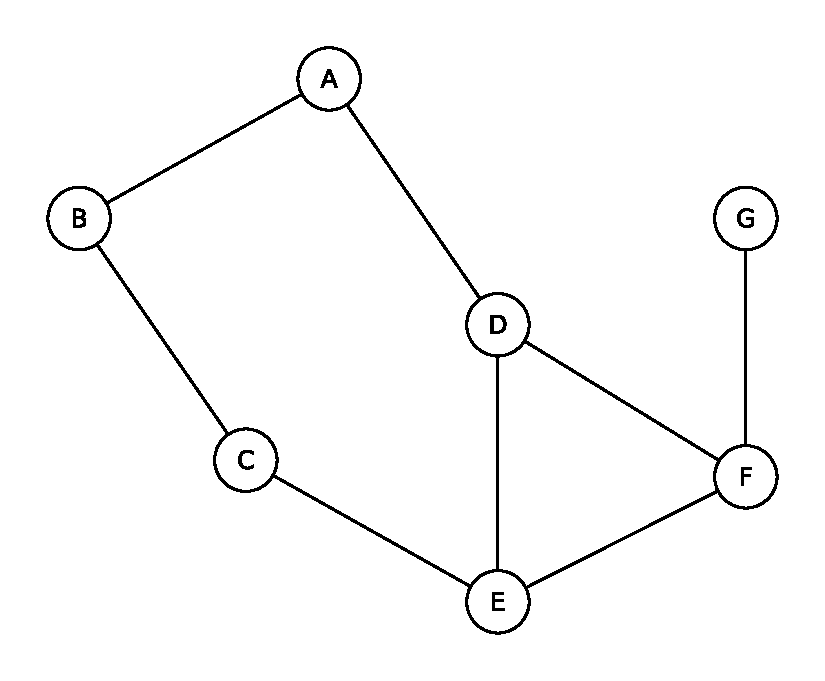
\includegraphics[scale=.55]{../imgs/coeficiente_agrupamento_1.eps}
    }%
    \subfloat[Depois de novas arestas se formarem]{%
      \label{fig:coeficiente_agrupamento_depois}
      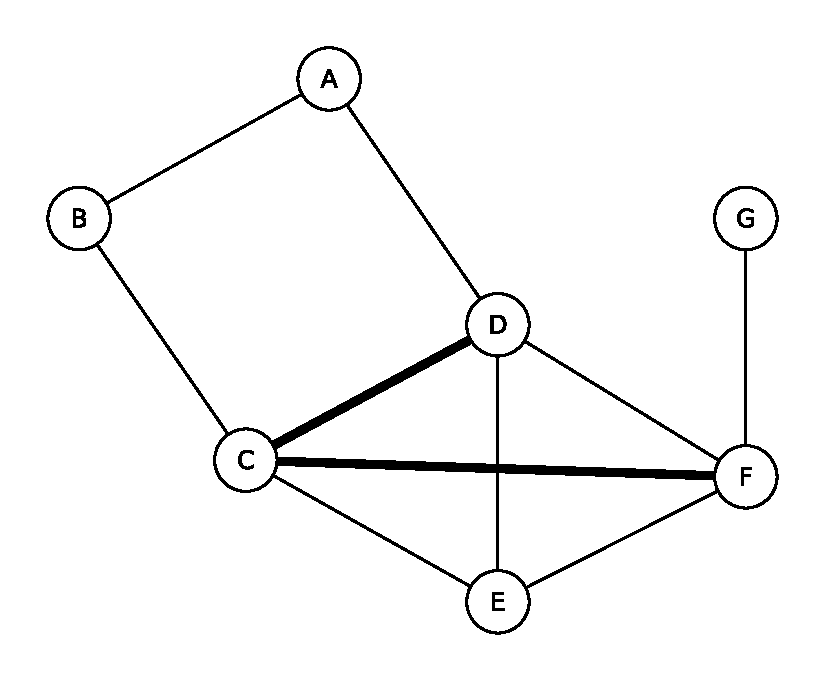
\includegraphics[scale=.55]{../imgs/coeficiente_agrupamento_2.eps}
    }%
  \end{center}
\caption{Exemplo de coeficiente de agrupamento}
\label{fig:averange_values_resemblance}
\end{figure}


%%%%%%%%%%%%%%%%%%%%%%%%%%%%%%%%%%%
\subsection{Componentes}
%%%%%%%%%%%%%%%%%%%%%%%%%%%%%%%%%%%

Segundo \cite{Easley2010}, um grafo é conectado quando existem arestas interligando todos os seus nodos. Naturalmente, 
um grafo é desconectado quando nem todos os seus nodos estão interligados, de modo que eles se dividem em grupos de nodos 
interconectados entre si, porém desconectados do restante da rede, sendo que dois grupos não se sobrepõem. Na 
Figura~\ref{fig:componentes_conectados}, podemos considerar que o grafo consiste de três partes, ou seja, três componentes
conectados: um composto pelos nodos \textit{K}, \textit{I}, \textit{J} e \textit{H}, outro composto pelos nodos 
\textit{L} e \textit{M} e o terceiro composto pelos demais nodos. Por exemplo, em uma rede de coautoria, poderíamos dizer
que cada componente é um grupo de pesquisa, sendo que os pesquisadores de um dado grupo não trabalham com pesquisadores
de outro grupo.

\cite{Easley2010} definem um componente conectado (\textit{connected component}), formalmente, como um subconjunto de 
nodos, tal que: (i) exista um caminho interligando todos os nodos daquele subconjunto e (ii) o subconjunto não é parte 
de um conjunto maior, onde cada nodo possa chegar a qualquer outro. Assim, podemos intuitivamente
definir que um componente é: (i) internamente conectado e (ii) como um todo, é uma ``parte'' 
desconectada das demais partes do grafo. Por exemplo, o subconjunto \textit{C}, \textit{F} e \textit{E} da 
Figura~\ref{fig:componentes_conectados} não poderia ser chamado de componente conectado, pois violaria a 
condição (ii). Embora o subconjunto atenda a condição (i), ele faz parte de um subconjunto maior que engloba 
o nodos de \textit{A} a \textit{G}.

\begin{figure}[!htb]
\centering
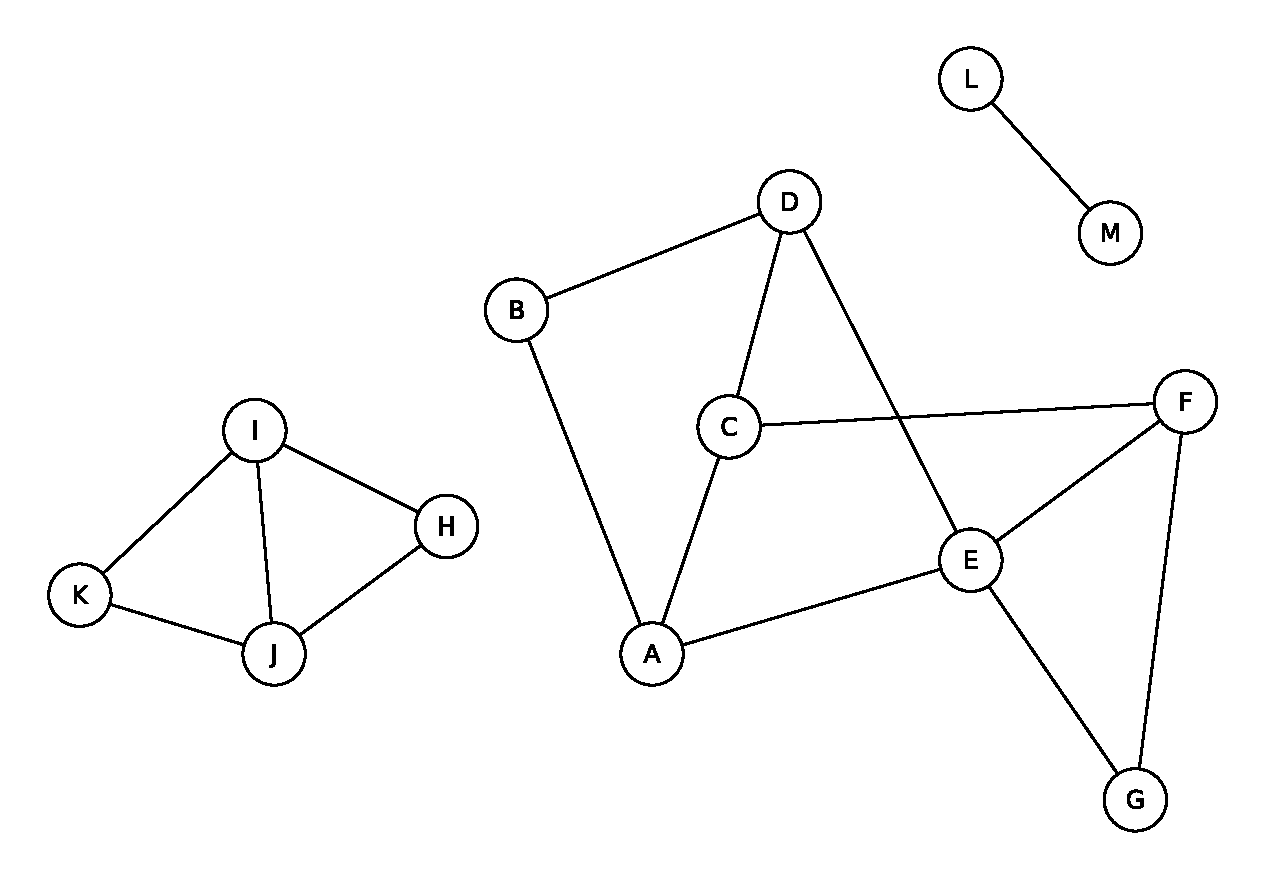
\includegraphics[scale=0.55]{../imgs/componentes.eps}
\caption{Um grafo com três componentes conectados}
\label{fig:componentes_conectados}
\end{figure}

Em um grafo direcionado, um componente é chamado de fortemente conectado quando existe pelo menos um caminho 
direcionado interligando todos os pares de nodos. Quando tal caminho existe, porém não direcionado, o componente 
é chamado de fracamente conectado. \cite{Benevenuto2012} exemplificam o modelo \textit{bow tie}, definido 
por \cite{Broder2000}, em que um grafo possui um componente central fortemente conectado, 
também chamado de \textit{core}, que pode ser alcançado ou alcançar outros grupos de componentes.

%%%%%%%%%%%%%%%%%%%%%%%%%%%%%%%%%%%
% \subsubsection{Maior Componente Conectado?}
%%%%%%%%%%%%%%%%%%%%%%%%%%%%%%%%%%%


%%%%%%%%%%%%%%%%%%%%%%%%%%%%%%%%%%%
\subsection{Caminho Mínimo Médio e Diâmetro}
%%%%%%%%%%%%%%%%%%%%%%%%%%%%%%%%%%%

Os caminhos de uma rede são um aspecto importante dela. Um caminho pode ser definido como uma sequência de nodos sem repetição
onde existe uma aresta entre cada par de nodos adjacentes na sequência. Por exemplo, na Figura~\ref{fig:componentes_conectados}
podemos dizer que existe um caminho entre \textit{A} e \textit{F}, sendo este caminho formado pelas arestas \textit{A-E} e 
\textit{E-F}. O comprimento de um caminho é dado pelo número de arestas que o define ou pelo número de nodos contidos no caminho
menos um. Ainda na Figura~\ref{fig:componentes_conectados}, o caminho contendo os nodos \textit{A}, \textit{B}, \textit{D}, \textit{C} e \textit{F} possui 
tamanho quatro.

Naturalmente existem muitos caminhos entre dois nodos quaisquer de um componente. Desta forma, o caminho mínimo entre
dois nodos é definido como sendo o comprimento do menor caminho entre eles. Assim, considerando os nodos  
\textit{A} e \textit{F} na Figura~\ref{fig:componentes_conectados}, o caminho mínimo entre eles é dois, definida pelos caminhos 
\textit{A}, \textit{C} e \textit{F} ou \textit{A}, \textit{E} e \textit{F}. 

O caminho mínimo médio de um grafo é a média do número de arestas em todos os caminhos mínimos existentes entre todos os pares 
de nodos do grafo. Geralmente esta medida é calculada no maior componente fortemente conectado para grafos direcionados ou no maior 
componente fracamente conectado para grafos não direcionados, uma vez que o grafo pode não ser totalmente conectado. \cite{Figueiredo2011} define 
o caminho mínimo médio como a média aritmética dos caminhos mínimos entre todos os pares de nodos da rede, sendo $l(i,j)$ o caminho mínimo entre os nodos
$i,j \in N$, onde $N$ é o conjuntos de nodos da rede. O caminho mínimo médio $\textit{\=l}$ é definido como:

\begin{equation}
\label{eq:distancia_media}
\textit{\=l} = \frac{\sum_{i,j \in N}{l(i,j)}}{\binom{n}{2}}.
\end{equation}

A Equação~\ref{eq:distancia_media} considera todos os pares não-ordenados, que ao todo são $\binom{n}{2}$. Outra métrica baseada 
em caminho mínimo é o diâmetro que também é calculado no maior componente fortemente conectado ou fracamente conectado. O 
diâmetro é o tamanho do maior caminho mínimo existente em todo o grafo, que \cite{Figueiredo2011} define como:

\begin{equation}
\label{eq:diametro}
\textit{L} = \max_{i,j\in N} l(i,j).
\end{equation}


%%%%%%%%%%%%%%%%%%%%%%%%%%%%%%%%%%%
\subsection{\textit{Betweenness}}
%%%%%%%%%%%%%%%%%%%%%%%%%%%%%%%%%%%

\textit{Betweenness} é uma métrica de centralidade que mede a importância de um determinado nodo ou aresta na rede 
referente à sua localização, considerando o número de caminhos mínimos que por ali passam. Nodos ou arestas com maior 
valor de \textit{betweenness} fazem parte de um número maior de caminhos mínimos e por isto são mais importantes na rede.

O valor da métrica \textit{betweenness} $B(e)$ de uma aresta $e$ pode, de acordo com \cite{Benevenuto2012}, ser formalmente definido como o 
número de caminhos mínimos entre todos os pares de nodos que passam por $e$. Desta forma temos:

\begin{equation}
\label{eq:betweenness}
B(e)=\sum_{u \in N, v \in N} \frac{\sigma_e (u,v)}{\sigma (u,v)}
\end{equation}
onde $\sigma (u,v)$ representa o número de caminhos mínimos entre $u$ e $v$, e $\sigma_e (u,v)$ representa o número de 
caminhos mínimos que incluem $e$. Assim, se existem vários caminhos mínimos entre $u$ e $v$, cada caminho recebe
um peso de modo que o somatório dos pesos seja um.

De forma análoga, o valor da métrica \textit{betweenness} pode ser computado para um nodo da rede ao invés de uma aresta. Assim teríamos
essa métrica representando a importância de um dado nodo para a rede, onde os vários caminhos mínimos que passam
por ele representam, de forma quantitativa, sua importância na rede. Por exemplo, em uma rede de coautoria, a existência de nodos com um alto valor
para a métrica \textit{betweenness} pode indicar que os respectivos pesquisadores atuam como pontes interligando vários grupos de pesquisa na rede. 
Desta forma, adotamos esta métrica de centralidade no restante da dissertação.

%%%%%%%%%%%%%%%%%%%%%%%%%%%%%%%%%%%
\subsection{Assortatividade}
%%%%%%%%%%%%%%%%%%%%%%%%%%%%%%%%%%%

A assortividade (\textit{assortativity} ou \textit{assortative mixing}) é uma métrica clássica de redes complexas que identifica
o comportamento de como os nodos tendem a se agrupar na rede, e.g., uma rede de coautoria apresenta propriedades assortativas 
quando pesquisadores com o mesmo número de conexões tendem a se conectar com outros pesquisadores com o mesmo número de conexões.

A assortatividade pode ser representada visualmente a partir de um gráfico em que cada grau $k$ encontrado em pelo menos um
nodo da rede é representado pelo grau médio $k_{nn}$ dos vizinhos dos nodos de grau $k$. Em grafos direcionados, este gráfico pode
ser construído separadamente para graus de entrada e graus de saída. Segundo \cite{Ahn2007}, esta métrica também pode ser expressa 
numericamente utilizando o coeficiente de correlação de Pearson:

\begin{equation}
\label{eq:assortatividade}
r = \frac{\langle k_ik_j \rangle-\langle k_i \rangle \langle k_j \rangle }
         {\sqrt{(\langle k^2_i \rangle - \langle k_i \rangle^2)(\langle k^2_j \rangle - \langle k_j \rangle^2)}}
\end{equation}
onde $k_i$ e $k_j$ são os graus dos nodos que constituem uma aresta e a notação $\langle \rangle$ representa a média sobre 
todas as arestas da rede.

Se a rede possui assortatividade negativa, nodos que possuem grau elevado tendem a se conectar a nodos com menor grau,
e vice versa. O coeficiente $r$ pode variar entre -1 e 1, onde $r > 0$ indica que a rede possui propriedades assortativas,
ou seja, nodos com graus semelhantes tendem a estabelecer conexões na rede, já $r < 0$ indica que a rede possui
propriedades disassortativas, existindo maior probabilidade de encontrar arestas entre nodos de graus diferentes.
Por exemplo, uma rede de coautoria com assortatividade negativa pode indicar que os pesquisadores seniores estão se
conectando a pesquisadores menos experientes, e.g., alunos de doutorado.

% %%%%%%%%%%%%%%%%%%%%%%%%%%%%%%%%%%%
\section{Modelos de Redes Complexas}
%%%%%%%%%%%%%%%%%%%%%%%%%%%%%%%%%%%

A análise de padrões em redes complexas instigaram vários trabalhos que tiveram como resultados modelos
que descrevem e caracterizam tais padrões. Nesta seção são descritos quatro modelos de redes complexas: 
redes aleatórias, redes \textit{small-world}, redes \textit{power-law} e livres de escala.

%%%%%%%%%%%%%%%%%%%%%%%%%%%%%%%%%%%
\subsection{Redes Aleatórias}
%%%%%%%%%%%%%%%%%%%%%%%%%%%%%%%%%%%

a

%%%%%%%%%%%%%%%%%%%%%%%%%%%%%%%%%%%
\subsection{Redes \textit{Small-World}}
%%%%%%%%%%%%%%%%%%%%%%%%%%%%%%%%%%%

%%%%%%%%%%%%%%%%%%%%%%%%%%%%%%%%%%%
\subsection{Redes \textit{Power-Law} e Livres de Escala}
%%%%%%%%%%%%%%%%%%%%%%%%%%%%%%%%%%%



%%%%%%%%%%%%%%%%%%%%%%%%%%%%%%%%%%%
\chapter{Comunidades}\label{comunidades}
%%%%%%%%%%%%%%%%%%%%%%%%%%%%%%%%%%%
% \redcomment{Revisar tradução e texto}
% Focar no Paper
Neste capítulo discutimos sobre as comunidades científicas que utilizamos em nossas análises e, em seguida, apresentamos
uma definição para identificação do que chamamos de núcleo das comunidades.

%%%%%%%%%%%%%%%%%%%%%%%%%%%%%%%%%%%
\section{Comunidades Científicas}
%%%%%%%%%%%%%%%%%%%%%%%%%%%%%%%%%%%

Dada uma rede social, uma comunidade pode ser compreendida como um grupo denso de nodos dessa rede que possuem mais arestas 
interligando-os entre si, do que arestas interligando-os ao restante da rede. Existem múltiplas definições e estratégias 
para identificar comunidades e elas variam de acordo com o contexto~\citep{Kleinberg2008,Leskovec2010}. No nosso contexto, 
uma comunidade científica pode ser definida em termos de uma grande e consolidada conferência científica capaz de reunir 
pesquisadores que trabalham em uma mesma área de pesquisa ao longo de vários anos.
% The notion of community can be understood as a dense group of nodes in a network, with more edges inside than edges linking the rest of the network.  There are multiple definitions
% and strategies of identifying communities and they vary according to the context~\cite{Kleinberg@cacm2008,Leskovec@www2010}. In our context, a scientific community is defined in terms of a large and well established
% scientific conference able to aggregate researchers working in similar research topics along a considerable number of years. 
 
A fim de construir um conjunto de comunidades científicas, coletamos dados da DBLP\footnote{http://dblp.uni-trier.de/}~\citep{Ley2009}, 
uma biblioteca digital que contém mais de 2,1 milhões de publicações de 1,2 milhões de autores e que provê informações 
bibliográficas dos principais anais de conferências e periódicos da área de Ciência da Computação. A DBLP disponibiliza 
todo o seu conjunto de dados no formato XML (\textit{eXtensible Markup Language}), o que facilita a obtenção dos dados e a 
construção de comunidades científicas inteiras.
% In order to construct a set of scientific communities, we have gathered data from DBLP\footnote{http://dblp.uni-trier.de/}~\cite{Ley:2009}, a digital library containing more
% than 2.1 million publications from 1.2 million authors that provides bibliographic information on major Computer Science conference proceedings and journals.  DBLP offers its
% entire database in XML format, which facilitates gathering and constructing entire scientific communities. 

Cada publicação é acompanhada por seu título, lista de autores, ano de publicação e veículo de publicação, i.e., conferência 
ou periódico. Para o propósito do nosso trabalho, consideramos uma comunidade científica como um grafo em que os nodos 
representam pesquisadores e as arestas ligam os coautores de artigos de uma mesma comunidade. A fim de definir tais 
comunidades, focamos nas publicações das principais conferências (\textit{flagship}) dos SIGs 
da ACM. Assim, definimos uma comunidade científica como formada por 
pesquisadores interligados entre si por serem coautores de um algum artigo dessas conferências, fazendo com 
que elas atuem como comunidades onde coautorias são formadas. Ao criarmos tais comunidades, removemos conferências 
sem dados suficientes para uma análise temporal, bem como conferências cujo histórico completo não está registrado 
na DBLP.
% Each publication is accompanied by its title, list of authors, year of publication, and publication venue, i.e., the conference or journal. For the purposes of our work, we
% consider a scientific community as a graph in which nodes represent researchers and edges links coauthors of papers from the same community.  In order to define such communities,
% we focus on the publications from the flagship conferences of major ACM SIGs (Special Interest Groups).  Thus, we define a scientific community by linking people that have
% coauthored a paper in a certain conference, making the flagship conferences of the ACM SIGs to act as communities where coauthorships are formed. We have removed young conferences
% without enough data for a temporal analysis as well as conferences whose entire history is not registered on DBLP to allow us carrying out temporal analyses. 

No total, 22 comunidades científicas foram construídas. A Tabela~\ref{tab:sigs_conference_period} lista essas comunidades, 
incluindo o respectivo SIG, acrônimo, período considerado (algumas conferências tiveram seu período 
reduzido para evitar hiato nos dados), número total de autores, publicações e edições, bem como razões extraídas desses 
três últimos dados.
% In total, 24 scientific communities were constructed. Table~\ref{tab:sigs_conference_period} lists these communities, including the respective ACM SIG, the conference acronym, the period
% considered (some conferences had the period reduced to avoid hiatus in the data), the total number of authors, publications and editions as well as ratios extracted from these last three figures.

\begin{table*}[!htb]
\centering
\caption{Estatísticas da DBLP das conferências \textit{flagship} dos SIGs da ACM }
\label{tab:sigs_conference_period}
{\fontsize{6.2}{10}\selectfont
\begin{tabular}{|l|l|c|c|c|c|c|c|c|c|} \hline
\textbf{SIG} & \textbf{Conferência} & \textbf{Período} & \textbf{Autores} & \textbf{Publicações} & \textbf{Edições} & \textbf{Aut/Edi} & \textbf{Pub/Edi} & \textbf{Aut/Pub}\\ \hline
SIGACT & STOC & 1969-2012 & 2159 & 2685 & 44 & 49,07 & 61,02 & 0,80\\ \hline
SIGAPP & SAC & 1993-2011 & 9146 & 4500 & 19 & 481,37 & 236,84 & 2,03\\ \hline
SIGARCH & ISCA & 1976-2011 & 2461 & 1352 & 36 & 68,36 & 37,56 & 1,82\\ \hline
SIGBED & HSCC & 1998-2012 & 846 & 617 & 15 & 56,40 & 41,13 & 1,37\\ \hline
SIGCHI & CHI & 1994-2012 & 5095 & 2819 & 19 & 268,16 & 148,37 & 1,81\\ \hline
SIGCOMM & SIGCOMM & 1988-2011 & 1593 & 796 & 24 & 66,38 & 33,17 & 2,00\\ \hline
SIGCSE & SIGCSE & 1986-2012 & 3923 & 2801 & 27 & 145,30 & 103,74 & 1,40\\ \hline
SIGDA & DAC & 1964-2011 & 8876 & 5693 & 48 & 184,92 & 118,60 & 1,56\\ \hline
SIGDOC & SIGDOC & 1989-2010 & 1071 & 810 & 22 & 48,68 & 36,82 & 1,32\\ \hline
SIGGRAPH & SIGGRAPH & 1985-2003 & 1920 & 1108 & 19 & 101,05 & 58,32 & 1,73\\ \hline
SIGIR & SIGIR & 1978-2011 & 3624 & 2687 & 34 & 106,59 & 79,03 & 1,35\\ \hline
SIGKDD & KDD & 1995-2011 & 3078 & 1699 & 17 & 181,06 & 99,94 & 1,81\\ \hline
SIGMETRICS & SIGMETRICS & 1981-2011 & 2083 & 1174 & 31 & 67,19 & 37,87 & 1,77\\ \hline
SIGMICRO & MICRO & 1987-2011 & 1557 & 855 & 25 & 62,28 & 34,20 & 1,82\\ \hline
SIGMM & MM & 1993-2011 & 5400 & 2928 & 19 & 284,21 & 154,11 & 1,84\\ \hline
SIGMOBILE & MOBICOM & 1995-2011 & 1151 & 480 & 17 & 67,71 & 28,24 & 2,40\\ \hline
SIGMOD & SIGMOD & 1975-2012 & 4202 & 2669 & 38 & 110,58 & 70,24 & 1,57\\ \hline
SIGOPS & PODC & 1982-2011 & 1685 & 1403 & 30 & 56,17 & 46,77 & 1,20\\ \hline
SIGPLAN & POPL & 1975-2012 & 1527 & 1217 & 38 & 40,18 & 32,03 & 1,25\\ \hline
SIGSAC & CCS & 1996-2011 & 1354 & 676 & 16 & 84,63 & 42,25 & 2,00\\ \hline
SIGSOFT & ICSE & 1987-2011 & 3502 & 2248 & 25 & 140,08 & 89,92 & 1,56\\ \hline
SIGWEB & CIKM & 1992-2011 & 4978 & 2623 & 20 & 248,90 & 131,15 & 1,90\\ \hline
\end{tabular}
}
\end{table*}
% \begin{table*}[!htb]
% \centering
% \caption{DBLP statistics on the flagship conferences of ACM SIGs}
% \label{tab:sigs_conference_period}
% {\small
% \begin{tabular}{|l|l|c|c|c|c|c|c|c|c|} \hline
% \bf{SIG} & \bf{Conference} & \bf{Period} & \bf{Authors} & \bf{Publications} & \bf{Editions} & \bf{Aut/Edi} & \bf{Pub/Edi} & \bf{Aut/Pub}\\ \hline
% SIGACT & STOC & 1969-2012 & 2159 & 2685 & 44 & 49.07 & 61.02 & 0.80\\ \hline
% SIGAPP & SAC & 1993-2011 & 9146 & 4500 & 19 & 481.37 & 236.84 & 2.03\\ \hline
% SIGARCH & ISCA & 1976-2011 & 2461 & 1352 & 36 & 68.36 & 37.56 & 1.82\\ \hline
% SIGBED & HSCC & 1998-2012 & 846 & 617 & 15 & 56.40 & 41.13 & 1.37\\ \hline
% SIGCHI & CHI & 1994-2012 & 5095 & 2819 & 19 & 268.16 & 148.37 & 1.81\\ \hline
% SIGCOMM & SIGCOMM & 1988-2011 & 1593 & 796 & 24 & 66.38 & 33.17 & 2.00\\ \hline
% SIGCSE & SIGCSE & 1986-2012 & 3923 & 2801 & 27 & 145.30 & 103.74 & 1.40\\ \hline
% SIGDA & DAC & 1964-2011 & 8876 & 5693 & 48 & 184.92 & 118.60 & 1.56\\ \hline
% SIGDOC & SIGDOC & 1989-2010 & 1071 & 810 & 22 & 48.68 & 36.82 & 1.32\\ \hline
% SIGGRAPH & SIGGRAPH & 1985-2003 & 1920 & 1108 & 19 & 101.05 & 58.32 & 1.73\\ \hline
% SIGIR & SIGIR & 1978-2011 & 3624 & 2687 & 34 & 106.59 & 79.03 & 1.35\\ \hline
% SIGKDD & KDD & 1995-2011 & 3078 & 1699 & 17 & 181.06 & 99.94 & 1.81\\ \hline
% SIGMETRICS & SIGMETRICS & 1981-2011 & 2083 & 1174 & 31 & 67.19 & 37.87 & 1.77\\ \hline
% SIGMICRO & MICRO & 1987-2011 & 1557 & 855 & 25 & 62.28 & 34.20 & 1.82\\ \hline
% SIGMM & MM & 1993-2011 & 5400 & 2928 & 19 & 284.21 & 154.11 & 1.84\\ \hline
% SIGMOBILE & MOBICOM & 1995-2011 & 1151 & 480 & 17 & 67.71 & 28.24 & 2.40\\ \hline
% SIGMOD & SIGMOD & 1975-2012 & 4202 & 2669 & 38 & 110.58 & 70.24 & 1.57\\ \hline
% SIGOPS & PODC & 1982-2011 & 1685 & 1403 & 30 & 56.17 & 46.77 & 1.20\\ \hline
% SIGPLAN & POPL & 1975-2012 & 1527 & 1217 & 38 & 40.18 & 32.03 & 1.25\\ \hline
% SIGSAC & CCS & 1996-2011 & 1354 & 676 & 16 & 84.63 & 42.25 & 2.00\\ \hline
% SIGSAM & ISSAC & 1988-2011 & 1100 & 1177 & 24 & 45.83 & 49.04 & 0.93\\ \hline
% SIGSOFT & ICSE & 1987-2011 & 3502 & 2248 & 25 & 140.08 & 89.92 & 1.56\\ \hline
% SIGUCCS & SIGUCCS & 1989-2011 & 1771 & 1593 & 23 & 77.00 & 69.26 & 1.11\\ \hline
% SIGWEB & CIKM & 1992-2011 & 4978 & 2623 & 20 & 248.90 & 131.15 & 1.90\\ \hline
% \end{tabular}
% }
% \end{table*}


%%%%%%%%%%%%%%%%%%%%%%%%%%%%%%%%%%%
\section{Definição do Núcleo das Comunidades}
%%%%%%%%%%%%%%%%%%%%%%%%%%%%%%%%%%%

Tentativas anteriores para identificar o núcleo de comunidades científicas são baseadas em abordagens 
algorítmicas que visam identificar conjuntos densos de nodos na rede~\citep{Seifi2012}. Entretanto, 
como planejamos investigar o papel do núcleo na estrutura da rede, qualquer abordagem que faz uso da 
estrutura da rede para identificar tais nodos poderia nos levar a um conjunto de pesquisadores 
enviesado. Em vez disso, focamos no desenvolvimento de uma métrica que quantificasse o envolvimento 
de um pesquisador em uma comunidade científica durante um certo período de tempo. Intuitivamente, 
essa métrica deveria ser capaz de capturar (i) a prolificidade de um pesquisador em diferentes 
comunidades e (ii) a frequência do envolvimento daquele pesquisador com a comunidade em um certo 
período de tempo.
% Previous attempts for identifying the community core of a scientific community are based on algorithmic approaches that aim at identifying dense clusters of nodes in the
% network~\cite{Seifi:2012:CCE:2187980.2188258}.  However, as we plan to investigate the role of a core in the network structure, any approach that makes use of the network structure
% to identify such nodes could lead us to a biased set of researchers. Instead, we focus on developing a metric that quantifies the involvement of a researcher in a scientific community
% during a certain period of time.  Intuitively, this metric should be able to capture (i) the prolificness of a researcher in different communities and (ii) the frequency of involvement
% of that researcher with the community in a certain period of time.

Em primeiro lugar, a fim de capturar a prolificidade de um pesquisador, usamos o índice~h~\citep{Hirsch2005}, 
uma métrica largamente adotada para esse propósito. Essa métrica consiste de um índice que tenta 
medir tanto a produtividade quanto o impacto dos trabalhos publicados de um dado pesquisador. Ela 
baseia-se no conjunto de artigos mais citados de um pesquisador e no número de citações 
desse pesquisador com pelo menos \textit{h} citações. Mais especificamente, um pesquisador tem um índice~h $i$ se publicou $i$ 
artigos que receberam pelo menos $i$ citações. Assim, por exemplo, se um pesquisador possui 
10 artigos com pelo menos 10 citações, seu índice~h final é 10.

% Mais especificamente, dado um período de tempo $t$, temos $t_i$ sendo o início deste 
% período e $t_f$ sendo seu final, um pesquisador $p$ em um dado instante de tempo $t_f$ tem 
% um índice~h $h_{p,t_f}$ se publicou $h$ artigos que receberam pelo menos \textit{h} citações 
% até esse instante de tempo $t_f$. Assim, por exemplo, se um pesquisador possui 10 artigos com pelo 
% menos 10 citações cada um ao longo do tempo, seu índice~h final é 10.

% First, in order to capture the prolificness of a researcher, we use the h-index~\cite{Hirsch:2005}, a metric widely adopted for this purpose. This metric consists of an index that
% attempts to measure both the productivity and the impact of the published work of a researcher. It is based on the set of the researcher's most cited papers and the number of
% citations that they have received.  More specifically, a researcher $r$ has an h-index $h_r$ if she has published \textit{h} papers which have received at least \textit{h} citations. Thus, for
% example, if a researcher has 10 papers with at least 10 citations, her h-index is 10.  

Em segundo lugar, como uma tentativa de capturar a importância de um pesquisador em uma comunidade 
específica em um certo período de tempo, multiplicamos o valor do seu índice~h 
ao final desse período pelo número de publicações desse pesquisador nessa comunidade 
no mesmo período. Denominamos essa métrica de \textit{Community Score} (\textit{CoScore}) \citep{Alves2013}. 
Mais formalmente, o \textit{CoScore} de um pesquisador $p$ em uma 
comunidade $c$ durante um período de tempo $t$, $\textit{CoScore}_{p,c,t}$, é dado 
pelo seu índice~h ($h_{p,t}$) ao final do período $t$ multiplicado pelo 
seu número de publicações na comunidade $c$ durante $t$ ($\textrm{\#}\text{publicações}_{p,c,t}$),
como expresso pela Equação~\ref{eq:core_score}.

\begin{equation}
  \label{eq:core_score}
  \textit{CoScore}_{p,c,t} = h_{p,t} \times \textrm{\#}\text{publicações}_{p,c,t}
\end{equation}

%Pontuação{ }do{ }Núcleo_{p,c,t} = h_p \times \textrm{\#}publicações_{p,c,t}
% Second, as an attempt to capture the importance of a researcher to a specific community in a certain period of time, we multiple her h-index by the number of publications this
% researcher has in a certain community during a time window. We name this measure \textit{Core Score}. More formally, the Core Score of a researcher $r$ in a community $c$ during a period of
% time $t$, $Core{ }Score_{r,c,t}$, is given by its h-index $h_r$ multiplied by the number of publications $r$ has in $c$ during $t$ ($\textrm{\#}publications_{r,c,t}$),
% as expressed by Equation~\ref{eq:core_score}. 
% \vspace{-0.01cm}
% \begin{equation} 
%   \label{eq:core_score}
%   Core{ }Score_{r,c,t} = h_r \times \textrm{\#}publications_{r,c,t}
% \end{equation}
% 
% %\begin{equation} 
% %  \label{eq:core_score}
% %  Core{ }Score_{a,c,t} = h\textrm{-}index_a \times number\textrm{ }of\textrm{ }publications_{a,c,t}
% %\end{equation}

Como podemos ver, a primeira parte da equação captura a importância de um pesquisador para 
a comunidade científica como um todo em um determinado período de tempo, independentemente 
de qualquer área de pesquisa específica, e a segunda parte pesa essa importância baseada na 
atividade do pesquisador em uma certa comunidade. A fim de computar o \textit{CoScore} para 
os membros de uma comunidade, definimos o núcleo de uma comunidade em um certo período de tempo 
como sendo formado pelos pesquisadores com o melhor escore naquela comunidade em termos de 
seu \textit{CoScore} em um dado período. 

A seguir, na Subseção~\ref{sub:hindex}, detalhamos como estimamos o índice~h dos pesquisadores 
ao longo do tempo. Então, na Subseção~\ref{sub:limiares}, discutimos como definimos dois 
importantes limiares: o tamanho do núcleo da comunidade e a janela de tempo usada em nossas análises.
% We note that the first part of the equation captures the importance of a researcher to the scientific community as a whole regardless any specific research area or period of time and the second part weights this
% importance based on the activity of the researcher in a certain community and time.  By computing the core score for the members of a community, we define the community core in a
% certain period of time as the top researchers of that community in terms of their core scores in the given period. Next, in Subsection~\ref{sub:hindex}, we detail how we inferred the
% h-index of researchers. 
% Then, in Subsection~\ref{sub:thresholds}, we discuss how we defined two important thresholds: the size of the community core and the time window used in our analyses.

%%%%%%%%%%%%%%%%%%%%%%%%%%%%%%%%%%%
\subsection{Estimativa do Índice H dos Pesquisadores}\label{sub:hindex}
%%%%%%%%%%%%%%%%%%%%%%%%%%%%%%%%%%%

Existem várias ferramentas que medem o índice~h de pesquisadores, das quais o Google 
Citations\footnote{http://scholar.google.com/citations} é a mais proeminente. No entanto, 
para ser incluído neste sistema, o pesquisador precisa se inscrever e criar explicitamente 
seu perfil. Em uma coleção preliminar com parte dos perfis de autores da DBLP, descobrimos 
que menos de 30\% desses autores tinham um perfil no Google Citations. Assim, esta estratégia 
poderia reduzir nosso conjunto de dados e, potencialmente, introduzir algum viés na análise 
das comunidades.
% There are multiple tools that measure the h-index of researchers, out of which Google Citations\footnote{http://scholar.google.com/citations} is the most prominent one.
% However, to have a profile in this system, a researcher needs to sign up and explicitly create her research profile.  In a preliminary collection of part of the profiles of
% the DBLP authors, we found that less than 30\% of these authors had a profile at Google citations. Thus, this strategy would reduce our dataset and
% potentially introduce bias when analyzing the communities.

Para evitar essa limitação, utilizamos os dados do projeto SHINE\footnote{http://shine.icomp.ufam.edu.br/}
(\textit{Simple HINdex Estimator}) para estimar o índice~h dos pesquisadores.
O SHINE fornece um \textit{website} que permite seus usuários verificar o índice~h de quase 
duas mil conferências de Ciência da Computação. Para isso, seus desenvolvedores realizaram 
uma coleta no Google Scholar\footnote{http://scholar.google.com}, buscando pelo título dos 
artigos publicados nessas conferências, o que lhes permitiu efetivamente estimar o índice~h 
das conferências alvo com base nas citações computadas pelo Google Scholar. Embora o SHINE 
permita somente consultas ao índice~h de conferências, seus desenvolvedores gentilmente nos 
permitiram acessar o seu conjunto de dados para estimarmos o índice~h dos pesquisadores 
baseados nas conferências coletadas. Embora isso possa gerar um viés em nossas estimativas, 
segundo \cite{Laender2008}, os pesquisadores da área de Ciência da Computação tendem a 
publicar cerca 2,5 artigos em conferências para cada artigo publicado em periódicos, contrabalançando
uma possível discrepância.
% To divert from this limitation, we used data from the SHINE (Simple HINdex Estimator) project\footnote{http://shine.icomp.ufam.edu.br/} to infer the researchers' h-index.
% SHINE provides a website that allows users to check the h-index of almost two thousands Computer Science conferences. They crawled Google Scholar, searching for the title of papers
% published in these conferences, which allowed them to effectively estimate the h-index of the target conferences based on the citations computed by Google Scholar. Although
% SHINE only allows one to search for the h-index of conferences, the SHINE developers kindly allowed us to access their dataset to infer the h-index of researchers based on the
% conferences they crawled.
% 

No entanto, existem duas importantes limitações com esta estratégia. A primeira limitação 
é referente ao dados coletados, uma vez que o SHINE não coleta todas as conferências 
existentes da área de Ciência da Computação, o índice~h dos pesquisadores pode ser 
subestimado quando calculado com esses dados. Para investigar esta questão, comparamos 
o índice~h de um conjunto de pesquisadores que possuem perfil no Google Citations, 
com seu índice~h estimado com base nos dados do SHINE. Para isso, selecionamos 
aleatoriamente 10 pesquisadores de cada conferência da Tabela~\ref{tab:sigs_conference_period} 
e extraímos o índice~h de seus perfis no Google Scholar. Em comparação com o índice~h 
que estimamos a partir dos dados do SHINE, os valores do Google Citations são, 
em média, 50\% maiores. A Figura~\ref{fig:hindex_scatter_plot} mostra o gráfico de 
dispersão para os dois índices h medidos. Podemos observar que, embora o índice~h 
calculado a partir dos dados do SHINE seja menor, as duas medidas são altamente 
correlacionadas. O coeficiente de correlação de Pearson é de 0,85, apresentando 
uma forte correlação positiva, o que indica que os pesquisadores podem ter seu 
índice~h proporcionalmente estimados em ambos os sistemas.

\begin{figure}[!htb]
\centering
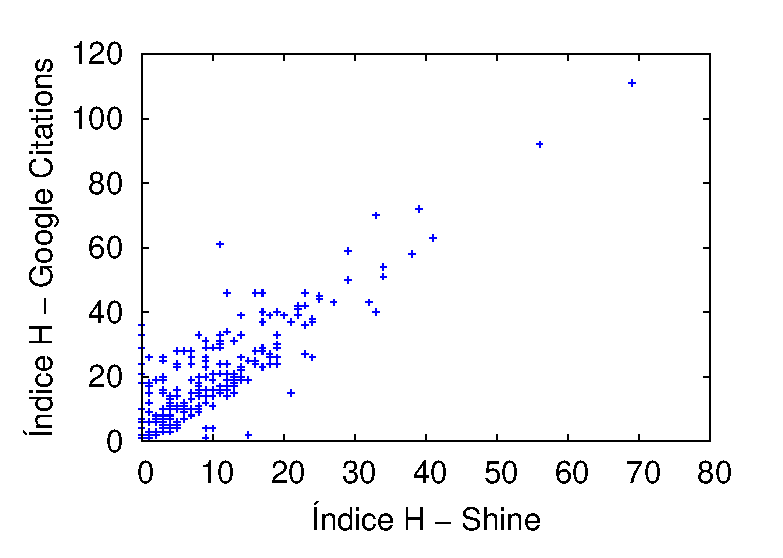
\includegraphics[scale=1]{../graficos/hindex/pt_BR/hindex_scatter_plot.eps}
\caption{Correlação entre o índice h estimado e o Google Citations}
\label{fig:hindex_scatter_plot}
\end{figure}
% \begin{figure}[!htb]
% \centering
% 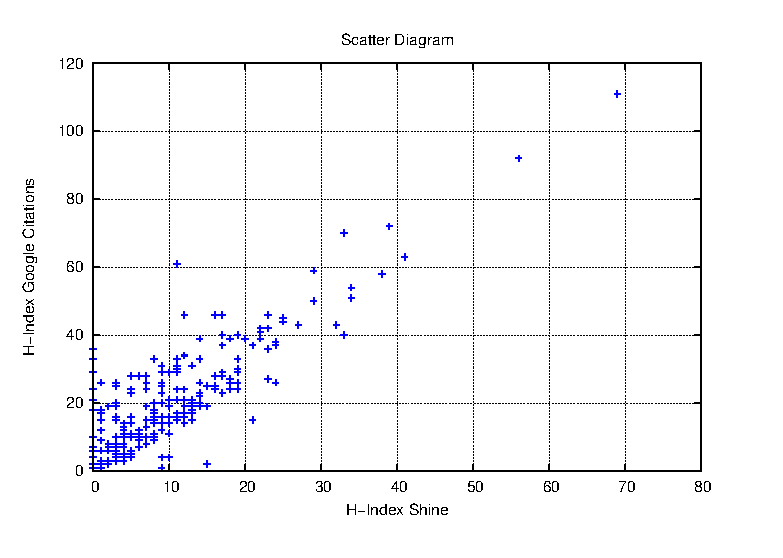
\includegraphics[scale=.5]{graficos/hindex/hindex_scatter_plot.eps}
% \caption{Correlation between the inferred h-index and Google Citations one}
% \vspace{-0.2cm}
% \label{fig:hindex_scatter_plot}
% \end{figure}
% 

% However, there is one important limitation with this strategy.  As SHINE does not track all the existent Computer Science conferences, researchers' h-index might be underestimated when computed
% with this data. To investigate this issue, we compared the h-index of a set of researchers with a profile on Google Scholar with their estimated h-index based on the SHINE data. For this, we
% randomly selected 10 researchers for each conference from Table~\ref{tab:sigs_conference_period} and extracted their h-indexes from their Google Scholar profiles.  In comparison
% with the h-index we estimated from SHINE, the Google Scholar values are, on average, 50\% higher. Figure~\ref{fig:hindex_scatter_plot} shows the scatter plot for the two h-index
% measures. We can note that although SHINE h-index is smaller, the two measures are highly correlated. The Pearson's correlation coefficient is 0.85, which indicates that researchers
% might have proportional h-index estimations in both systems. 

A segunda limitação está relacionada à evolução do índice~h ao longo do tempo. O 
SHINE coleta somente o total atual de citações de cada artigo, sendo possível estimar 
apenas o valor final do índice~h de um dado pesquisador. De forma análoga à abordagem 
anterior, selecionamos aleatoriamente 10 pesquisadores de cada conferência e extraímos 
do Google Citations o número de citações dos artigos de cada pesquisador ao longo 
do tempo, nos permitindo, assim, obter a curva de evolução do índice~h desses pesquisadores.

\cite{Acuna2012} apresentam um método que inclui equações capazes de predizer o índice~h 
de um pesquisador daqui a um, cinco ou dez anos. Desta forma, 
utilizamos cada equação para estimar o índice~h dos pesquisadores e comparamos com os 
dados coletados do Google Citations utilizando regressão linear, $R^2$. De acordo com 
a CDF (\textit{Cumulative Distribution Function}) na Figura~\ref{fig:calculos_nature}, 
podemos observar que a equação de um ano é a que mais se assemelha aos valores do Google
Citations, tendo mais de 70\% dos pesquisadores com $R^2$ superior a 60\%. Com base 
nas equações definidas por \cite{Acuna2012}, computamos o índice~h dos pesquisadores
utilizando três abordagens: (i) a primeira fixa o índice~h atual do pesquisador ao 
longo do tempo, (ii) em seguida utilizamos a equação capaz de prever o índice~h ano a ano 
dos pesquisadores definida por \cite{Acuna2012}, e (iii) por fim, utilizamos uma 
evolução linear do índice~h do pesquisador considerando a sua primeira e última data de publicação.
A Figura~\ref{fig:comprativo_evolucao_hindex} mostra a CDF da $R^2$ entre os valores 
do Google Scholar e os valores estimados utilizando as três abordagens propostas, sendo 
possível observar que a abordagem utilizando a evolução linear é a que mais se 
aproxima dos valores do Google Scholar, tendo mais de 60\% dos pesquisadores com $R^2$ superior a 80\%.

% \redcomment{Como base nos dados coletados, utilizamos três abordagens com o intuito de observar qual melhor representa a evolução do índice~h a partir do seu valor final. A primeira abordagem mantém 
% constante o índice~h final do pesquisador ao longo do tempo. Em seu trabalho, \cite{Acuna2012} apresentam três abordagens capazes de predizer o índice~h de um pesquisador, desta forma, 
% usamos cada método para estimar o índice~h dos pesquisadores, conforme apresentado na Figura~\ref{fig:calculos_nature}, sendo possível observar, de acordo com a CDF (\textit{Cumulative 
% Distribution Function}) da regressão linear, $R^2$, que a abordagem que prevê o índice~h ano a ano apresenta um melhor resultado, sendo esta apontada como a nossa segunda abordagem. 
% Por fim, a terceira e última abordagem consiste em utilizar uma evolução linear do índice~h do pesquisador considerando a sua primeira e última data de publicação. A 
% Figura~\ref{fig:comprativo_evolucao_hindex} mostra a CDF da $R^2$ entre os valores do Google Scholar e os valores estimados utilizando as três abordagens propostas, sendo 
% possível observar que a abordagem utilizando a evolução linear é a que mais se aproxima dos valores do Google Scholar, tendo mais de 60\% dos pesquisadores
% com valor superior a 80\% a $R^2$.}

\begin{figure}[!htb]
  \begin{center}
    \subfloat[Valores gerados utilizando o método proposto por \cite{Acuna2012}]{%
      \label{fig:calculos_nature}
      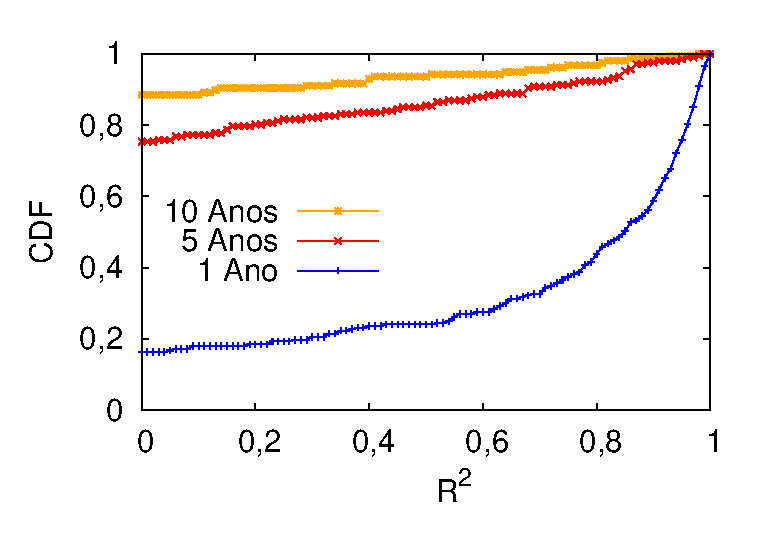
\includegraphics[scale=.5]{../graficos/hindex/pt_BR/nature_cdf.eps}
    }%
    \hspace{1cm}
    \subfloat[Valores gerados utilizando as três estratégias]{%
      \label{fig:comprativo_evolucao_hindex}
      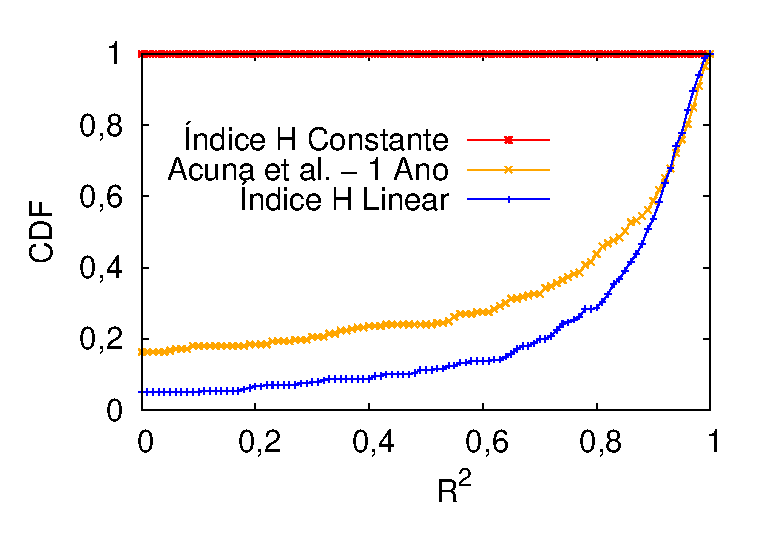
\includegraphics[scale=.5]{../graficos/hindex/pt_BR/linear_hindex_cdf.eps}
    }%
  \end{center}
  \caption{Evolução do índice~h}
  \label{fig:evolucao_hindex}
\end{figure}

%%%%%%%%%%%%%%%%%%%%%%%%%%%%%%%%%%%
\subsection{Definição dos Limiares}\label{sub:limiares}
%%%%%%%%%%%%%%%%%%%%%%%%%%%%%%%%%%%

Nossa estratégia para definir os dois limiares necessários para definir o núcleo das 
comunidades consiste em variar cada um deles e quantificar como eles impactam nas 
mudanças dos membros desse núcleo. Para medir essas mudanças, calculamos a
métrica \textit{resemblance}, conforme definida por~\cite{Viswanath2009}, que mede a 
fração dos membros do núcleo no tempo $t_0$ que permanecem no núcleo no tempo $t_1$.
Para cada comunidade, variamos o tamanho da janela de 1 a 5 anos e o tamanho do 
núcleo de 10\% a 60\% do total dos respectivos pesquisadores.
% Our strategy to define the two required thresholds consists of varying each of them and quantifying how they impact on the changes on the members of the community core. To measure these
% changes, we compute the resemblance metric, as used in~\cite{Viswanath:2009}, which measures the fraction of members in the core at time $t_0$ that remains in the core at time $t_1$. 
% For each community, we varied the window size from 1 to 5 years and the size of the community core from 10\% to 60\% of the entire community.
% % 
% % There are two important thresholds in our approach we need to define to determine the core of a scientific community.  The first is related to the time window in which the 
% % community core is computed. In other words, should we compute the community core at each year, at each two years, or for a larger time window? The second threshold is related to the
% % size of the community core. As we define the core of a community as the top researchers in terms of their core score during a certain time window, it is important to define the
% % threshold for choosing the top ones.

Intuitivamente, uma alta variação da métrica \textit{resemblance} indica uma escolha 
ruim dos limiares. Assim, procuramos por limiares cujas mudanças causassem pequenas 
alterações nos valores dessa métrica. A Figura~\ref{fig:averange_values_resemblance} 
mostra os valores do \textit{resemblance} em função do tamanho da janela, fornecendo 
diferentes curvas para o tamanho do núcleo da comunidade. Mostramos aqui apenas as 
curvas das comunidades SIGMOD e CHI, as curvas das demais comunidades podem ser encontradas 
no Apêndice~\ref{apendice:media_valores_resemblance}. Por inspeção visual definiríamos 
o tamanho do núcleo da comunidade como 10\% devido à proximidade das curvas e o tamanho 
da janela como 2 ou 3, uma vez que a maior parte das comunidades mostra um valor 
do \textit{resemblance} mais estável após esses valores. Para nos ajudar a decidir, calculamos 
o coeficiente angular das curvas com tamanho do núcleo de 10\% para cada comunidade e a 
média do coeficiente angular para elas. Com base nesses valores, definimos o tamanho da 
janela para nossos experimentos como sendo de 3 anos.
% Intuitively, high resemblance variations indicate bad threshold choices and, thus, we should seek for values in which threshold changes cause slight changes on resemblance.
% Figure~\ref{fig:averange_values_resemblance} shows the resemblance values as a function of the window size, providing different curves for the community core size.  We chose the
% SIGMOD and CHI communities for this analysis. The rest of the communities are omitted due to lack of space, but the same observations hold for them. By visual inspection we would set the core
% size as 10\% due to the proximity of the curves, and the window size as 2 or 3, as most of the communities showed a more stable resemblance after these values. To help us decide, we
% computed the angular coefficient for the 10\% core size curves of each community and obtained the average angular coefficient for them.  Based on this value, we chose the window
% size for our experiments as 3 years.

\begin{figure}[!htb]
  \begin{center}
    \subfloat[SIGMOD]{%
      \label{fig:sigmod_slide_window_top_list}
      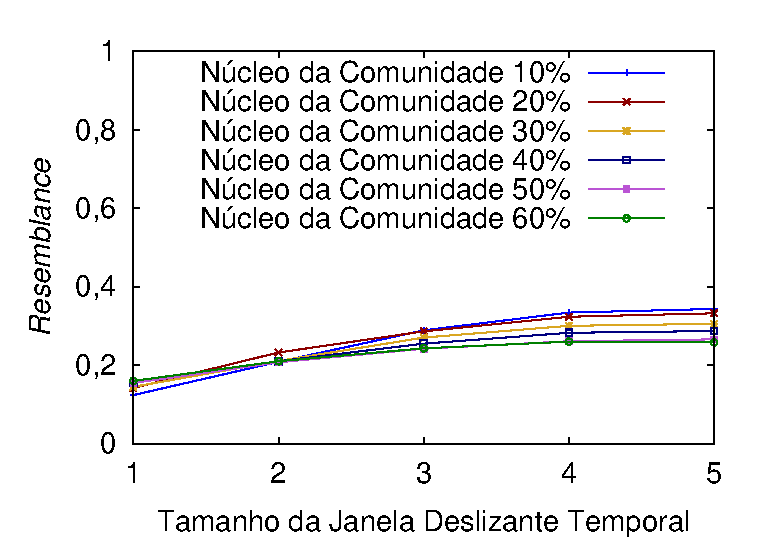
\includegraphics[scale=.6]{../graficos/window_core_size/pt_BR/sigmod_conference_arithmetic_slide_window_arithmetic_top_list.eps}
    }%
    \subfloat[CHI]{%
      \label{fig:chi_slide_window_top_list}
      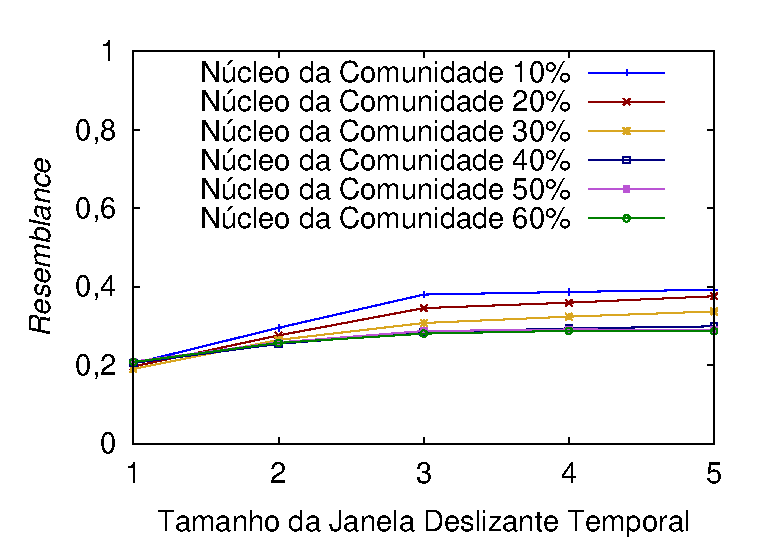
\includegraphics[scale=.6]{../graficos/window_core_size/pt_BR/chi_arithmetic_slide_window_arithmetic_top_list.eps}
    }%
  \end{center}
\caption{Média dos valores de \textit{resemblance}}
\label{fig:averange_values_resemblance}
\end{figure}
% \begin{figure}[!htb]
%   \begin{center}
%     \subfigure[SIGMOD]{%
%       \label{fig:sigmod_slide_window_top_list}
%       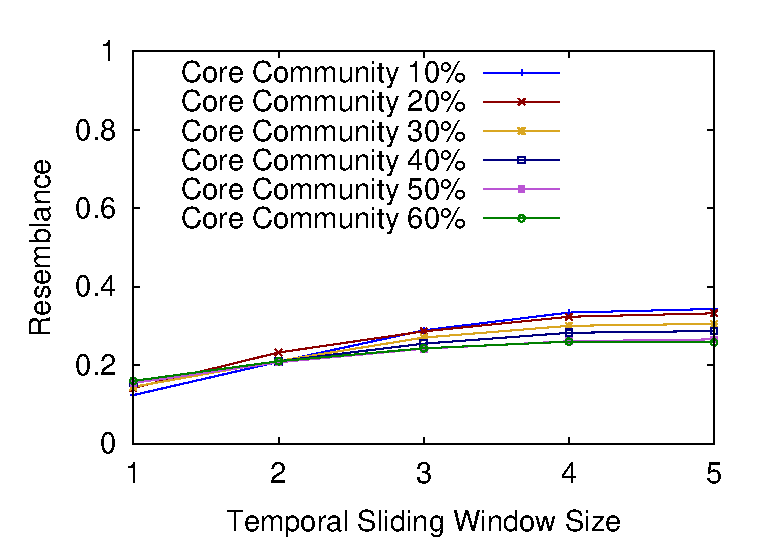
\includegraphics[scale=.33]{graficos/window_core_size/sigmod_slide_window_top_list.eps}
%     }%
%     \subfigure[CHI]{%
%       \label{fig:chi_slide_window_top_list}
%       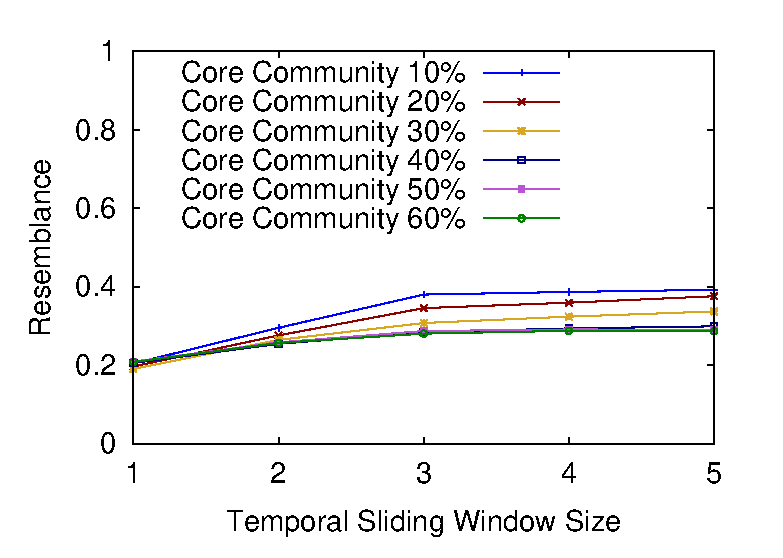
\includegraphics[scale=.33]{graficos/window_core_size/chi_slide_window_top_list.eps}
%     }%
%   \end{center}
% \vspace{-0.5cm}
% \caption{Average of the values of resemblance}
%  \label{fig:averange_values_resemblance}
% \end{figure}
% 

%%%%%%%%%%%%%%%%%%%%%%%%%%%%%%%%%%%
\subsection{Validação}
%%%%%%%%%%%%%%%%%%%%%%%%%%%%%%%%%%%

Com base no \textit{CoScore}, esperamos que os membros do núcleo da comunidade sejam pesquisadores que contribuam ativamente com publicações em uma determinada comunidade.
A validação desta suposição é, por natureza, subjetiva. Assim, fornecemos a seguir evidências que nossa abordagem captura corretamente essa característica esperada.
% Based on the core score value, we expect that the members of the community core would be standing researchers that actively contribute with publications to a certain community.
% The validation of this assumption is, by nature, subjective.  Thus, we provide next evidence that our approach correctly captures this expected characteristic.

\begin{figure}[!htb]
  \begin{center}
    \subfloat[Jon Kleinberg]{%
      \label{fig:cc_kleinberg}
      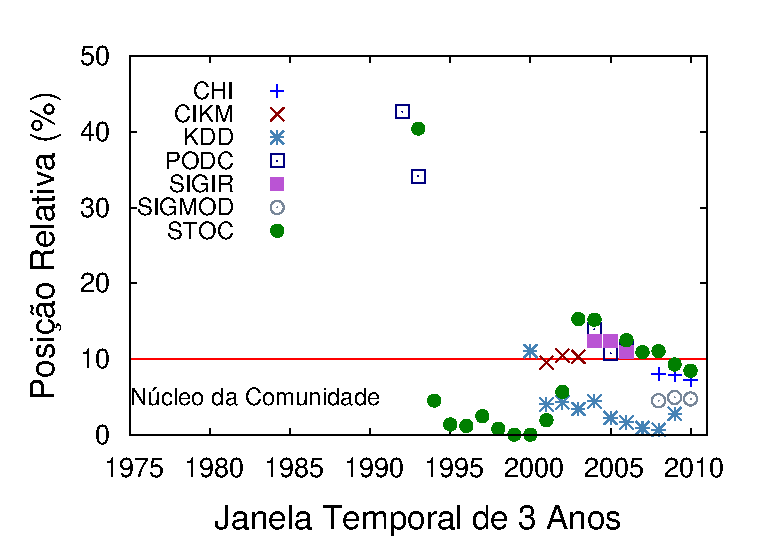
\includegraphics[scale=.6]{../graficos/validacao_core_community/pt_BR/cc_kleinberg_evolution.eps}
    }%
    \subfloat[Luis von Ahn]{%
      \label{fig:cc_luis_von_ahn}
      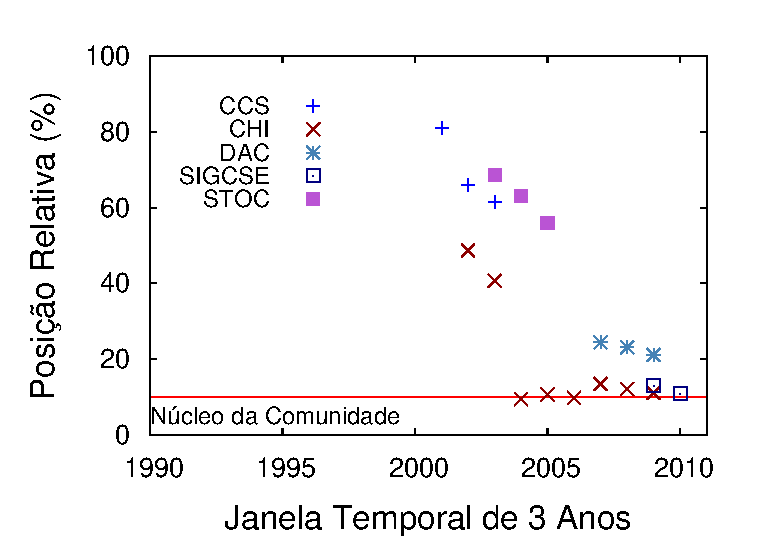
\includegraphics[scale=.6]{../graficos/validacao_core_community/pt_BR/cc_luis_von_ahn_evolution.eps}
    }%
  \end{center}
\caption{\textit{CoScore} de dois palestrantes convidados da WWW 2013}
 \label{fig:rank_core_score_authors}
\end{figure}

% \begin{figure}[!htb]
%   \begin{center}
%     \subfigure[Jon Kleinberg]{%
%       \label{fig:cc_kleinberg}
%       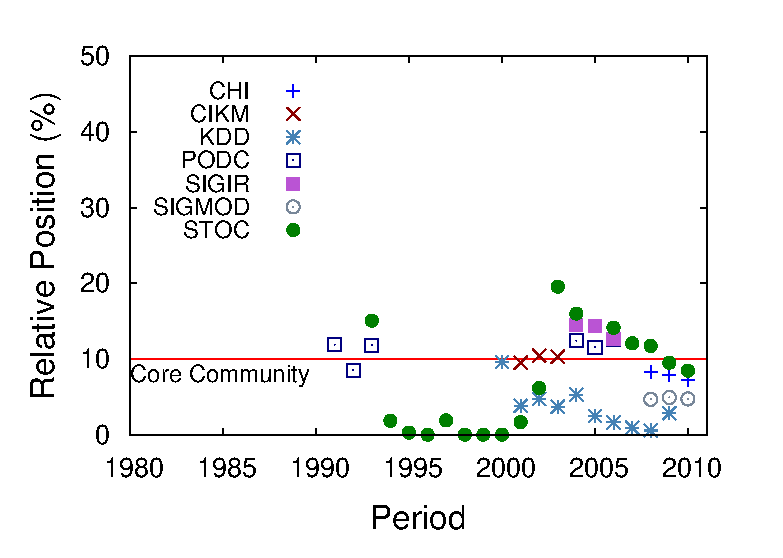
\includegraphics[scale=.33]{graficos/validacao_core_community/cc_kleinberg.eps}
%     }%
%     \subfigure[Luis von Ahn]{%
%       \label{fig:cc_luis_von_ahn}
%       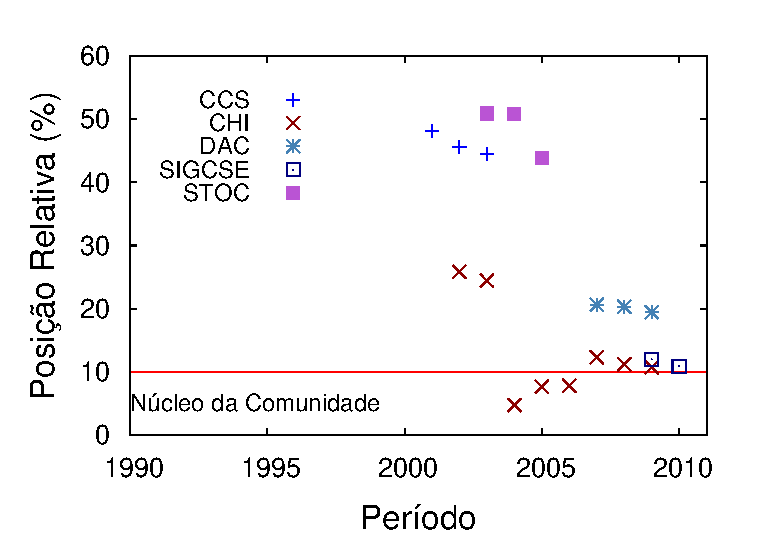
\includegraphics[scale=.33]{graficos/validacao_core_community/cc_luis_von_ahn.eps}
%     }%
%   \end{center}
% \vspace{-0.5cm}
% \caption{Core score of two WWW 2013 keynote speakers}
%  \label{fig:rank_core_score_authors}
% \end{figure}
% 

Primeiro, analisamos o \textit{CoScore} de dois palestrantes convidados da 
conferência WWW 2013 realizada recentemente no Rio de Janeiro: Jon Kleinberg 
e Luis von Ahn. A Figura~\ref{fig:rank_core_score_authors} mostra 
a posição em termos da percentagem (e.g., a posição 5\% de uma dada comunidade), 
desses dois pesquisadores nas comunidades em que eles têm publicado. A linha inferior 
divide os membros do núcleo da comunidade dos demais membros. Podemos notar que Jon 
Kleinberg foi membro do núcleo da comunidade STOC, uma conferência teórica, por anos. Mais 
precisamente, ele foi parte do núcleo da STOC por doze anos, publicando sete artigos 
na STOC em um único período de três anos. Com o envolvimento de Kleinberg na KDD, ele se tornou 
menos ativo na STOC e saiu do núcleo dessa comunidade por algum tempo. Durante esse 
período, ele publicou muitos artigos na KDD, enquanto suas publicações na STOC foram 
reduzindo. Com relação ao pesquisador Luis von Ahn, podemos notar que ele é mais ativo 
na comunidade CHI, na qual ele publicou seis artigos ao longo de sua vida acadêmica. Ele 
chegou ao núcleo da comunidade CHI em duas janelas de tempo, publicando quatro artigos 
na CHI em um único período.

% Primeiro, nós analisamos a pontuação do núcleo de dois palestrantes principais da WWW 2013: Jon Kleinberg e Luis von Ahn. A Figura~\ref{fig:rank_core_score_authors} mostra 
% a posição no ranking em termos da porcentagem (e.g., a posição 5\% de uma dada comunidade) destes dois pesquisadores nas comunidades que eles tenham publicado. A linha inferior 
% divide os membros do núcleo da comunidade dos demais membros. Nós podemos notar que Jon Kleinberg era um membro do núcleo da comunidade STOC, uma conferência teórica, por anos. Mais 
% precisamente, ele foi parte do núcleo da STOC por doze anos, publicando sete artigos na STOC em um único período de três anos. Com o envolvimento de Kleinberg na KDD, ele se tornou 
% menos ativo na STOC e saiu do núcleo dessa comunidade por algum tempo. Durante este período, ele publicou muitos artigos na KDD, enquanto suas publicações na STOC foram 
% reduzindo. Quando se trata de Luis von Ahn, nós podemos notar que ele é mais ativo na comunidade CHI, uma comunidade em que ele publicou seis artigos ao longo de sua vida 
% acadêmica. Ele chegou ao núcleo da comunidade CHI ao longo de três janelas de tempo consecutivas, publicando quatro artigos na CHI em um único período.

% First, we analyzed the core score of two WWW 2013 keynote speakers: Jon Kleinberg and Luis von Ahn.  Figure~\ref{fig:rank_core_score_authors} shows the ranking position in terms of
% percentage (e.g., position 5\% of that community) of these two researchers in the communities they have published. The bottom line divides the members of the community core from the others.
% We can note that Jon Kleinberg was a member of the community core of STOC, a theoretical conference, for years. More precisely, he was part of the STOC core for twelve years,
% publishing seven STOC papers in a single period of three years. With Kleinberg's involvement on KDD, he became less active in STOC and left the core of that community for some time.
% During this period, he published several KDD papers, while his STOC publications were reduced.  When it comes to Luis von Ahn, we can note that he is more active in
% the CHI community, a community in which he published six papers along his academic life. He reached the core of the CHI community along three consecutive time windows,
% publishing four CHI papers in a single period.


\begin{table*}[!hptb]
\centering
\caption{Pesquisadores das conferências CHI, ICSE, KDD e POPL que apareceram com mais 
frequência no núcleo da comunidade através dos anos.}
\label{tab:authors_frequency_core_community_grupo1}
{\fontsize{9.2}{11}\selectfont
\begin{tabular}{|c|c|c|c|} \hline
\textbf{CHI} & \textbf{ICSE} & \textbf{KDD} & \textbf{POPL}\\ \hline
\textbf{Scott E. Hudson} & \textbf{Victor R. Basili} & \textbf{Heikki Mannila} & Thomas W. Reps\\ \hline
\textbf{Hiroshi Ishii} & \textbf{Barry W. Boehm} & Hans-Peter Kriegel & Martín Abadi\\ \hline
\textbf{Steve Benford} & \textbf{Jeff Kramer} & \textbf{Jiawei Han} & John C. Mitchell\\ \hline
\textbf{George G. Robertson} & \textbf{Mary Shaw} & Martin Ester & Robert Harper\\ \hline
\textbf{Shumin Zhai} & Dewayne E. Perry & \textbf{Rakesh Agrawal} & Zohar Manna\\ \hline
\textbf{Brad A. Myers} & Don S. Batory & Bing Liu & Benjamin C. Pierce\\ \hline
\textbf{Robert E. Kraut} & Mary Jean Harrold & Ke Wang & Amir Pnueli$^\star$\\ \hline
\textbf{Elizabeth D. Mynatt} & \textbf{Lori A. Clarke} & \textbf{Padhraic Smyth} & \textbf{Barbara Liskov}$^\star$\\ \hline
\textbf{Ravin Balakrishnan} & Gruia-Catalin Roman & Philip S. Yu & Martin C. Rinard\\ \hline
\textbf{James A. Landay} & Premkumar T. Devanbu & Charu C. Aggarwal & Luca Cardelli\\ \hline
Ken Hinckley & Gail C. Murphy & \textbf{Vipin Kumar} & Thomas A. Henzinger\\ \hline
\textbf{Mary Czerwinski} & \textbf{Richard N. Taylor} & Wynne Hsu & \textbf{Ken Kennedy}\\ \hline
\textbf{Carl Gutwin} & \textbf{David Garlan} & Qiang Yang & \textbf{Matthias Felleisen}\\ \hline
\textbf{Gregory D. Abowd} & Michael D. Ernst & \textbf{Christos Faloutsos} & Edmund M. Clarke$^\star$\\ \hline
Michael J. Muller & James D. Herbsleb & William W. Cohen & Mitchell Wand\\ \hline
\textbf{Susan T. Dumais} & Lionel C. Briand & Pedro Domingos & David Walker\\ \hline
Loren G. Terveen & Gregg Rothermel & Eamonn J. Keogh & Simon L. Peyton Jones\\ \hline
\textbf{Steve Whittaker} & Kevin J. Sullivan & Alexander Tuzhilin & Shmuel Sagiv\\ \hline
W. Keith Edwards & \textbf{David Notkin} & Mohammed Javeed Zaki & Barbara G. Ryder\\ \hline
\textbf{John M. Carroll} & Douglas C. Schmidt & Mong-Li Lee & Alexander Aiken\\ \hline
\end{tabular}
% \par\medskip\footnotesize{$^\star$ Pesquisadores premiados por uma vida de inovação e liderança dentro daquela comunidade.}
% \par\medskip\footnotesize{$^\star$ Pesquisadores agraciados com \textit{A. M. Turing Award}.}
}
\end{table*}


\begin{table*}[!hptb]
\centering
\caption{Pesquisadores das conferências SIGCOMM, SIGGRAPH, SIGIR e SIGMOD que apareceram com mais 
frequência no núcleo da comunidade através dos anos.}
\label{tab:authors_frequency_core_community_grupo2}
{\fontsize{9.2}{11}\selectfont
\begin{tabular}{|c|c|c|c|} \hline
\textbf{SIGCOMM} & \textbf{SIGGRAPH} & \textbf{SIGIR} & \textbf{SIGMOD}\\ \hline
\textbf{Scott Shenker} & \textbf{Donald P. Greenberg} & \textbf{W. Bruce Croft} & \textbf{Michael Stonebraker}\\ \hline
George Varghese & \textbf{Pat Hanrahan} & Clement T. Yu & \textbf{David J. DeWitt}\\ \hline
\textbf{Donald F. Towsley} & Demetri Terzopoulos & \textbf{Gerard Salton} & \textbf{Philip A. Bernstein}\\ \hline
Ion Stoica & \textbf{David Salesin} & Alistair Moffat & H. V. Jagadish\\ \hline
Hui Zhang & \textbf{Michael F. Cohen} & \textbf{Susan T. Dumais} & Christos Faloutsos\\ \hline
Deborah Estrin & \textbf{Richard Szeliski} & James Allan & \textbf{Rakesh Agrawal}\\ \hline
Hari Balakrishnan & John F. Hughes & Yiming Yang & \textbf{Michael J. Carey}\\ \hline
Robert Morris & N. Magnenat-Thalmann & Edward A. Fox & \textbf{H. Garcia-Molina}\\ \hline
Thomas E. Anderson & \textbf{Tomoyuki Nishita} & James P. Callan & Jiawei Han\\ \hline
Ramesh Govindan & \textbf{Andrew P. Witkin} & Chris Buckley & Raghu Ramakrishnan\\ \hline
Srinivasan Seshan & Norman I. Badler & \textbf{C. J. van Rijsbergen} & Jeffrey F. Naughton\\ \hline
David Wetherall & \textbf{Peter Schröder} & Justin Zobel & \textbf{Jim Gray}$^\star$\\ \hline
Yin Zhang & Steven Feiner & Ellen M. Voorhees & Hans-Peter Kriegel\\ \hline
Jennifer Rexford & \textbf{Hugues Hoppe} & Mark Sanderson & Gerhard Weikum\\ \hline
Jia Wang & \textbf{Jessica K. Hodgins} & \textbf{Norbert Fuhr} & Philip S. Yu\\ \hline
J. J. Garcia-Luna-Aceves & \textbf{Greg Turk} & Nicholas J. Belkin & Divesh Srivastava\\ \hline
Randy H. Katz & \textbf{Marc Levoy} & Chengxiang Zhai & Joseph M. Hellerstein\\ \hline
Albert G. Greenberg & \textbf{P. Prusinkiewicz} & Charles L. A. Clarke & Krithi Ramamritham\\ \hline
Mark Handley & Eihachiro Nakamae & Alan F. Smeaton & Nick Roussopoulos\\ \hline
\textbf{Simon S. Lam} & Dimitris N. Metaxas & Gordon V. Cormack & \textbf{Surajit Chaudhuri}\\ \hline
\end{tabular}
% \par\medskip\footnotesize{$^\star$ Pesquisadores premiados por uma vida de inovação e liderança dentro daquela comunidade.}
% \par\medskip\footnotesize{$^\star$ Pesquisadores agraciados com \textit{A. M. Turing Award}.}
}
\end{table*}

% CHI
% 52 90 0.577777777778
% ICSE
% 15 23 0.652173913043
% KDD
% 9 12 0.75
% POPL
% 6 23 0.260869565217
% SIGCOMM
% 9 26 0.346153846154
% SIGGRAPH
% 21 42 0.5
% SIGIR
% 7 10 0.7
% SIGMOD
% 17 20 0.85

% \begin{table*}[!hptb]
% \centering
% \caption{Pesquisadores que apareceram com mais frequência no núcleo da comunidade através dos anos.}
% \label{tab:authors_frequency_core_community}
% {\fontsize{9.2}{11}\selectfont
% \begin{tabular}{|c|c|c|c|} \hline
% \textbf{KDD} & \textbf{SIGCOMM} & \textbf{SIGIR} & \textbf{SIGMOD}\\ \hline
% Heikki Mannila$^\star$ & Scott Shenker$^\star$ & W. Bruce Croft$^\star$ & David J. DeWitt$^\star$\\ \hline
% Jiawei Han$^\star$ & George Varghese & Clement T. Yu & Michael Stonebraker$^\star$\\ \hline
% Eamonn J. Keogh & Hui Zhang & Susan T. Dumais$^\star$ & H. V. Jagadish\\ \hline
% Martin Ester & Donald F. Towsley$^\star$ & James Allan & Rakesh Agrawal$^\star$\\ \hline
% Bing Liu & Hari Balakrishnan & Justin Zobel & Christos Faloutsos\\ \hline
% Padhraic Smyth$^\star$ & Ion Stoica & Alistair Moffat & Raghu Ramakrishnan\\ \hline
% Charu C. Aggarwal & Srinivasan Seshan & Norbert Fuhr$^\star$ & Jiawei Han\\ \hline
% Philip S. Yu & Deborah Estrin & James P. Callan & Gerhard Weikum\\ \hline
% Ke Wang & David Wetherall & Yiming Yang & Philip A. Bernstein$^\star$\\ \hline
% Hans-Peter Kriegel & Thomas E. Anderson & Edward A. Fox & Jeffrey F. Naughton\\ \hline
% Rakesh Agrawal$^\star$ & Jennifer Rexford & Gerard Salton$^\star$ & Hector Garcia-Molina$^\star$\\ \hline
% Jian Pei & Jia Wang & Ricardo A. Baeza-Yates & Michael J. Carey$^\star$\\ \hline
% Wynne Hsu & Ratul Mahajan & Jian-Yun Nie & Joseph M. Hellerstein\\ \hline
% Qiang Yang & Vern Paxson$^\star$ & Mark Sanderson & Philip S. Yu\\ \hline
% Christos Faloutsos$^\star$ & Mark Handley & Charles L. A. Clarke & Divesh Srivastava\\ \hline
% Huan Liu & Yin Zhang & Chris Buckley & Michael J. Franklin\\ \hline
% Mohammed Javeed Zaki & Peter Steenkiste & Chengxiang Zhai & Jennifer Widom$^\star$\\ \hline
% Pedro Domingos & Walter Willinger & Alan F. Smeaton & Hans-Peter Kriegel\\ \hline
% Jon M. Kleinberg & Ramesh Govindan & Zheng Chen & Hamid Pirahesh\\ \hline
% Vipin Kumar$^\star$ & Jon Crowcroft$^\star$ & Ophir Frieder & Surajit Chaudhuri$^\star$\\ \hline
% \end{tabular}
% \par\medskip\footnotesize{$^\star$ Pesquisadores premiados por uma vida de inovação e liderança dentro daquela comunidade.}
% }
% \end{table*}
% ----------------------
% \begin{table*}[!hptb]
% \centering
% \caption{Researchers who appear most often in the community core over the years}
% \label{tab:authors_frequency_core_community}
% {\small
% \begin{tabular}{|c|c|c|c|} \hline
% \bf{KDD} & \bf{SIGCOMM} & \bf{SIGIR} & \bf{SIGMOD}\\ \hline
% Heikki Mannila$^\star$ & Scott Shenker$^\star$ & W. Bruce Croft$^\star$ & David J. DeWitt$^\star$\\ \hline
% Jiawei Han$^\star$ & George Varghese & Clement T. Yu & Michael Stonebraker$^\star$\\ \hline
% Eamonn J. Keogh & Hui Zhang & Susan T. Dumais$^\star$ & H. V. Jagadish\\ \hline
% Martin Ester & Donald F. Towsley$^\star$ & James Allan & Rakesh Agrawal$^\star$\\ \hline
% Bing Liu & Hari Balakrishnan & Justin Zobel & Christos Faloutsos\\ \hline
% Padhraic Smyth$^\star$ & Ion Stoica & Alistair Moffat & Raghu Ramakrishnan\\ \hline
% Charu C. Aggarwal & Srinivasan Seshan & Norbert Fuhr$^\star$ & Jiawei Han\\ \hline
% Philip S. Yu & Deborah Estrin & James P. Callan & Gerhard Weikum\\ \hline
% Ke Wang & David Wetherall & Yiming Yang & Philip A. Bernstein$^\star$\\ \hline
% Hans-Peter Kriegel & Thomas E. Anderson & Edward A. Fox & Jeffrey F. Naughton\\ \hline
% Rakesh Agrawal$^\star$ & Jennifer Rexford & Gerard Salton$^\star$ & Hector Garcia-Molina$^\star$\\ \hline
% Jian Pei & Jia Wang & Ricardo A. Baeza-Yates & Michael J. Carey$^\star$\\ \hline
% Wynne Hsu & Ratul Mahajan & Jian-Yun Nie & Joseph M. Hellerstein\\ \hline
% Qiang Yang & Vern Paxson$^\star$ & Mark Sanderson & Philip S. Yu\\ \hline
% Christos Faloutsos$^\star$ & Mark Handley & Charles L. A. Clarke & Divesh Srivastava\\ \hline
% Huan Liu & Yin Zhang & Chris Buckley & Michael J. Franklin\\ \hline
% Mohammed Javeed Zaki & Peter Steenkiste & Chengxiang Zhai & Jennifer Widom$^\star$\\ \hline
% Pedro Domingos & Walter Willinger & Alan F. Smeaton & Hans-Peter Kriegel\\ \hline
% Jon M. Kleinberg & Ramesh Govindan & Zheng Chen & Hamid Pirahesh\\ \hline
% Vipin Kumar$^\star$ & Jon Crowcroft$^\star$ & Ophir Frieder & Surajit Chaudhuri$^\star$\\ \hline
% \end{tabular}
% \par\medskip\footnotesize{$^\star$ Researchers awarded by a lifetime of innovation and leadership inside that community.}
% }
% \vspace{-0.2cm}
% \end{table*}
% 

Em seguida, computamos a posição dos pesquisadores que aparecem com mais 
frequência no núcleo de suas comunidades científicas. Escolhemos 
as conferências CHI, ICSE, KDD, POPL, SIGCOMM, SIGIR e SIGMOD para 
mostrar os 20 pesquisadores melhores colocados, conforme destacado nas
Tabelas~\ref{tab:authors_frequency_core_community_grupo1}~e~\ref{tab:authors_frequency_core_community_grupo2}. 
Como podemos notar, vários pesquisadores renomados aparecem no topo dessas 
listas, incluindo os palestrantes convidados das últimas edições das respectivas 
conferências e pesquisadores premiados por suas contribuições naquelas comunidades, 
cujos nomes aparecem em negrito, incluindo alguns que também receberam o ACM \textit{A.M. 
Turing Award}\footnote{http://amturing.acm.org/byyear.cfm} (marcados com $^\star$). De fato, analisando os pesquisadores premiados 
de cada comunidade, descobrimos que grande parte deles apareceu no núcleo da 
comunidade pelo menos uma vez na história da conferência. Mais especificamente, estas 
frações são de 58\% dos membros premiados da CHI\footnote{http://www.sigchi.org/about/awards}, 
65\% para a ICSE\footnote{http://www.sigsoft.org/awards/outResAwd.htm}, 75\% para a 
KDD\footnote{http://www.sigkdd.org/awards\_innovation.php}, 26\% para a 
POPL\footnote{http://www.sigplan.org/Awards/Achievement/Main}, 35\% para a 
SIGCOMM\footnote{http://www.sigcomm.org/awards/sigcomm-awards}, 50\% para a 
SIGGRAPH\footnote{http://www.siggraph.org/participate/awards}, 70\% para a
SIGIR\footnote{http://www.sigir.org/awards/awards.html}, e 85\% para a 
SIGMOD\footnote{http://www.sigmod.org/sigmod-awards}. Exceto para as conferências SIGCOMM 
e POPL (SIGPLAN), cujos SIGs patrocinam outros eventos que não foram considerados 
em nosso conjunto de dados, as outras seis comunidades apresentam um número muito 
alto de membros premiados que aparecem pelo menos uma vez em seus respectivos 
núcleos. Além disso, podemos observar que a comunidade POPL possui pelo menos três 
pesquisadores que receberam o ACM \textit{A.M. Turing Award}, 
um dos mais importantes prêmios da comunidade científica. Estas observações fornecem evidências 
que nossa abordagem captura corretamente a noção do núcleo de uma comunidade científica.

% Em seguida, nós calculamos o ranking dos pesquisadores que aparecem com mais frequência no núcleo da comunidade de cada comunidade científica. Nós escolhemos 
% as conferências KDD, SIGCOMM, SIGIR e SIGMOD para mostrar seus 20 pesquisadores melhores colocados, conforme apresentado na Tabela~\ref{tab:authors_frequency_core_community}. Como 
% podemos notar, vários grandes nomes aparecem no topo da lista, incluindo os principais palestrantes das últimas edições destas comunidades, bem como pesquisadores 
% premiados por seu tempo de vida de constribuições naquela comunidades. De fato, analizando os pesquisadores premiados de cada comunidade, nós descobrimos que
% grande parte deles apareceram no núcleo da comunidade pelo menos uma vez na história da conferênica. Mais especificamente, estas frações são de 75\% dos membros premiados 
% da KDD\footnote{http://www.sigkdd.org/awards\_innovation.php}, 35\% para a SIGCOMM\footnote{http://www.sigcomm.org/awards/sigcomm-awards}, 60\% para a
% SIGIR\footnote{http://www.sigir.org/awards/awards.html}, e 80\% para a SIGMOD\footnote{http://www.sigmod.org/sigmod-awards}. Exceto para a SIGCOMM, uma comunidade 
% com muitos eventos patrocinados que não foram considerados em nosso conjunto de dados, as outras três comunidades apresentam um número muito alto de membros premiados 
% que aparecem pelo menos uma vez no núcleo da comunidade. Estas observações fornecem evidências que nossa abordagem captura corretamente a noção de um núcleo em comunidades científicas.

% Then, we computed a ranking of researchers that appear most often in the community core of each scientific community. We chose the KDD, SIGCOMM, SIGIR, and SIGMOD communities to
% show their top 20 researchers in Table~\ref{tab:authors_frequency_core_community}.  As we can note, several big names appear in this top list, including past keynote speakers of
% these conferences as well as awarded researchers by their life time contributions in that community. Indeed, by analyzing the awarded researchers from each community we found that
% a large fraction of them appeared in the community core at least one time in the conference history. More specifically, these fractions are 75\% of the awarded
% KDD\footnote{http://www.sigkdd.org/awards\_innovation.php} members, 35\% for SIGCOMM\footnote{http://www.sigcomm.org/awards/sigcomm-awards}, 60\% for
% SIGIR\footnote{http://www.sigir.org/awards/awards.html}, and 80\% for SIGMOD\footnote{http://www.sigmod.org/sigmod-awards}.  Except for SIGCOMM, a community with many sponsored
% events that were not considered in our datasets, the other three communities presented very high numbers of awarded members that appear at least one time in the community core. These
% observations provide evidence that our approach correctly captures the notion of a scientific community core.
%%%%%%%%%%%%%%%%%%%%%%%%%%%%%%%%%%%
\chapter{Análise das Comunidades}\label{analise-nucleo-comunidades}
%%%%%%%%%%%%%%%%%%%%%%%%%%%%%%%%%%%

Neste capítulo apresentamos uma série de análises sobre as comunidades científicas. Primeiro, analisamos como as 
propriedades dessas comunidades evoluem. Em seguida, comparamos, ao longo do tempo, as propriedades dos membros do núcleo 
com os demais membros das comunidades. Finalmente, calculamos a média do \textit{CoScore} das comunidades
para investigar variações nas propriedades dos núcleos e correlacionar essas variações com as propriedades das comunidades.

% In this section, we present a series of analyses about the scientific community cores. First, we analyze how the network properties 
% of the scientific communities have evolved. 
% Then, we contrast the properties of the community cores over time against the properties of the remaining members of the 
% respective communities. 
% Finally, we compute the average core score of a community to investigate fluctuations in the properties of the members of 
% the community cores and 
% correlate these fluctuations with the network properties of the communities.

%%%%%%%%%%%%%%%%%%%%%%%%%%%%%%%%%%%
\section{Evolução das Comunidades}\label{sub:evolucao_comunidades_cientifica}
%%%%%%%%%%%%%%%%%%%%%%%%%%%%%%%%%%%

A fim de estudar a evolução das principais propriedades estruturais das comunidades científicas, examinamos várias métricas 
de redes para cada uma das comunidades consideradas. Apresentamos aqui cinco métricas populares: assortatividade, caminho 
mínimo médio (CMM), coeficiente de agrupamento (CA), tamanho do maior componente fracamente conectado 
(CFC) e grau médio dos nodos. As Figuras~\ref{fig:metrics_largest_connected_component},
\ref{fig:metrics_average_shortest}, \ref{fig:metrics_clustering_coefficient}, \ref{fig:metrics_assortativity} e \ref{fig:metrics_average_degree}
mostram como cada uma dessas cinco métricas variam ao longo do tempo. Apresentamos essas métricas para um conjunto de seis 
comunidades científicas selecionadas entre aquelas que mais se estendem ao longo do tempo em nosso conjunto de dados.
Nossas análises são realizadas sob duas perspectivas. A primeira consiste em analisar a evolução da rede ano a ano, acumulando 
nodos e arestas da instância final do grafo. Essa perspectiva nos permite observar a estrutura final de uma 
comunidade em função do tempo. A segunda perspectiva consiste em analisar instâncias construídas com base em nodos e 
arestas criados em uma janela de tempo predefinida (três anos, tal como discutido na Subsecção~\ref{sub:limiares}). Esta análise 
nos permite investigar as variações da rede com potencial para impactar a sua estrutura final.
Os resultados da análise são semelhantes para as outras comunidades e podem ser observados no 
Apêndice~\ref{apendice:metricas_evolucao_comunidades}.

% In order to study the evolution of the main structural properties of the scientific communities, we examine 
% various network metrics for each of the scientific communities. We present four popular metrics here: assortativity, 
% clustering coefficient (CC), average shortest path (ASP), 
% and the size of the largest weakly connected component (WCC). Figure~\ref{fig:metrics} shows how each of these four metrics vary over time
% for a set of six scientific communities selected among those that span over the longest period in our dataset.  Our analyses are performed under two perspectives. The first
% consists on analyzing the network evolution year by year by accumulating nodes and edges to a single final snapshot of the graph. This perspective allows us to observe the final
% network structure of a community as a function of time. The second perspective consists of analyzing snapshots constructed based on nodes and edges created on a predefined time
% window (three years, as discussed in Subsection~\ref{sub:thresholds}). This analysis allows us to investigate network variations with potential to impact the final network structure.
% Our analysis results are similar for the other communities, but we omit them due to lack of space.

\begin{figure}[!htb]
  \begin{center}
  \subfloat[Maior CFC final]{%
    \label{fig:largest_connected_component_1_in_1}
    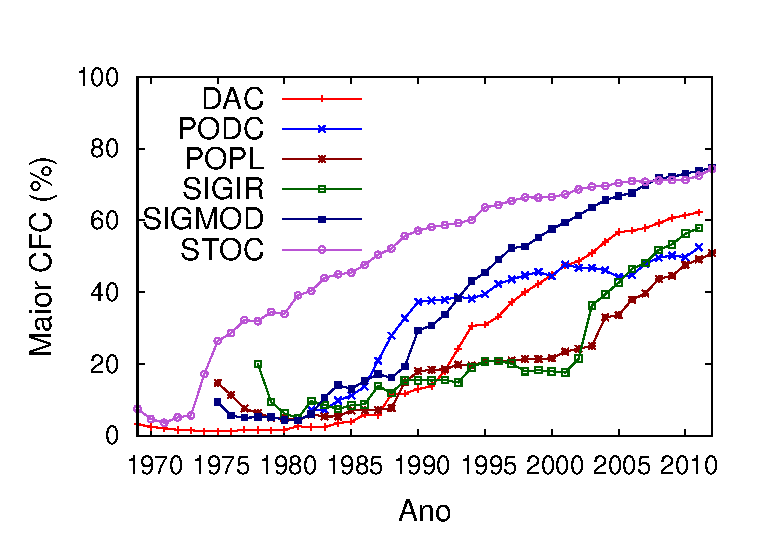
\includegraphics[scale=.6]{../graficos/sigs_metricas_acumuladas_1_em_1_ano/pt_BR/porcentagem_maior_componente_grupo_temporal_web.eps}
  }%
  \subfloat[Maior CFC por janela]{%
    \label{fig:largest_connected_component_slide_window}
    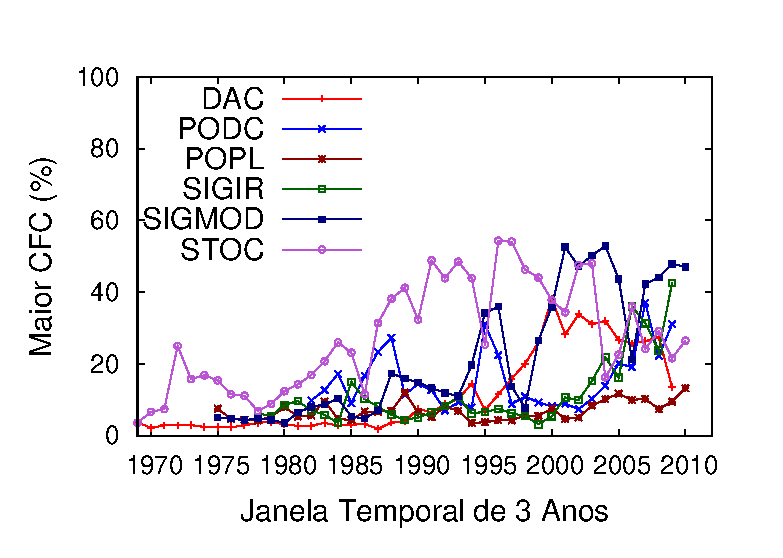
\includegraphics[scale=.6]{../graficos/core_over_time/metricas_tradicionais/pt_BR/porcentagem_maior_componente_slide_window_grupo_temporal_web.eps}
  }%
  \end{center}
  \caption{Maior CFC das comunidades científicas}
  \label{fig:metrics_largest_connected_component}
\end{figure}

\begin{figure}[!htb]
  \begin{center}
  \subfloat[CMM final]{%
    \label{fig:average_shortest_path_1_in_1}
    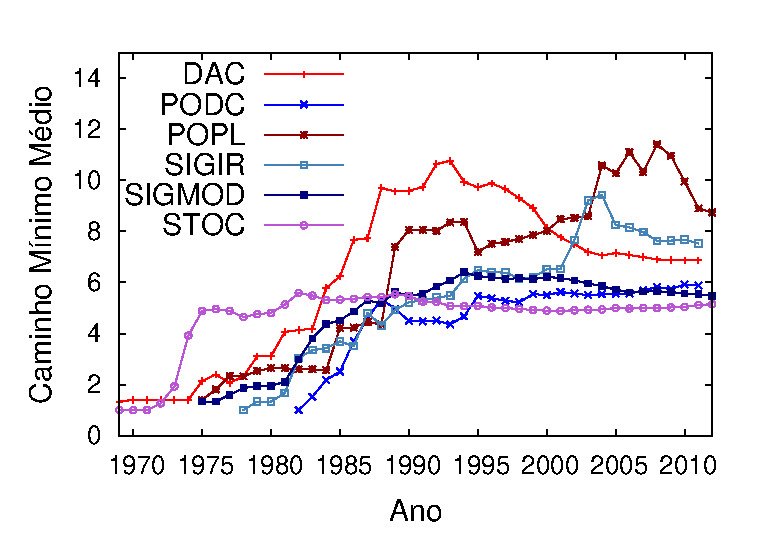
\includegraphics[scale=.6]{../graficos/sigs_metricas_acumuladas_1_em_1_ano/pt_BR/caminho_minimo_medio_grupo_temporal_web.eps}
  }%
  \subfloat[CMM por janela]{%
    \label{fig:average_shortest_path_slide_window}
    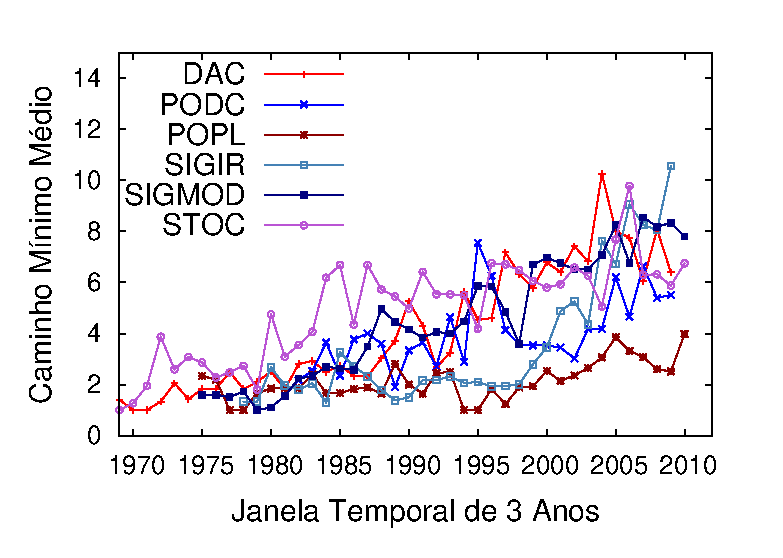
\includegraphics[scale=.6]{../graficos/core_over_time/metricas_tradicionais/pt_BR/caminho_minimo_medio_slide_window_grupo_temporal_web.eps}
  }%
  \end{center}
  \caption{Caminho mínimo médio das comunidades científicas}
  \label{fig:metrics_average_shortest}
\end{figure}

\begin{figure}[!htb]
  \begin{center}
  \subfloat[CC final]{%
    \label{fig:clustering_coefficient_1_in_1}
    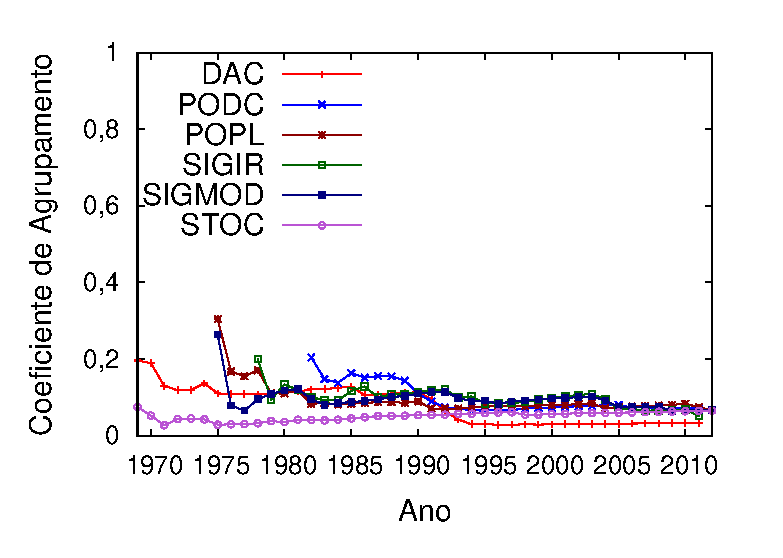
\includegraphics[scale=.6]{../graficos/sigs_metricas_acumuladas_1_em_1_ano/pt_BR/coeficiente_agrupamento_grupo_temporal_web.eps}
  }%
  \subfloat[CC por janela]{%
    \label{fig:clustering_coefficient_slide_window}
    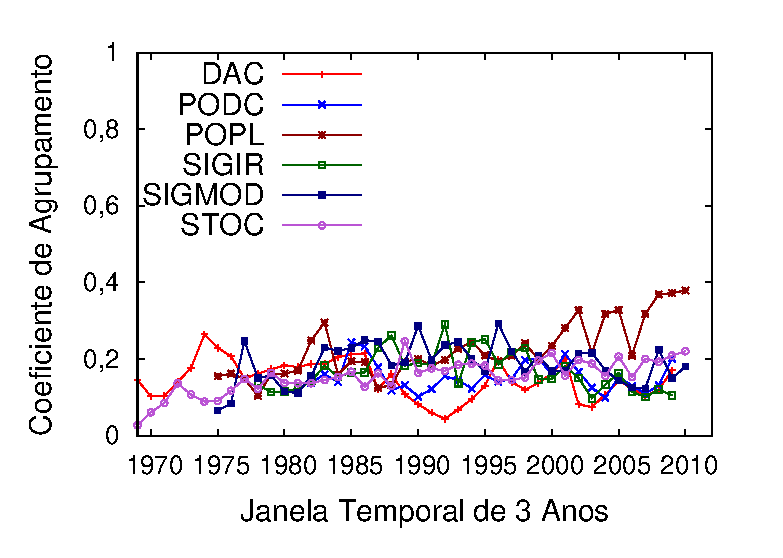
\includegraphics[scale=.6]{../graficos/core_over_time/metricas_tradicionais/pt_BR/coeficiente_agrupamento_slide_window_grupo_temporal_web.eps}
  }%
  \end{center}
  \caption{Coeficiente de agrupamento das comunidades científicas}
  \label{fig:metrics_clustering_coefficient}
\end{figure}

\begin{figure}[!htb]
  \begin{center}
  \subfloat[Assortatividade final]{%
    \label{fig:assortativity_1_in_1}
    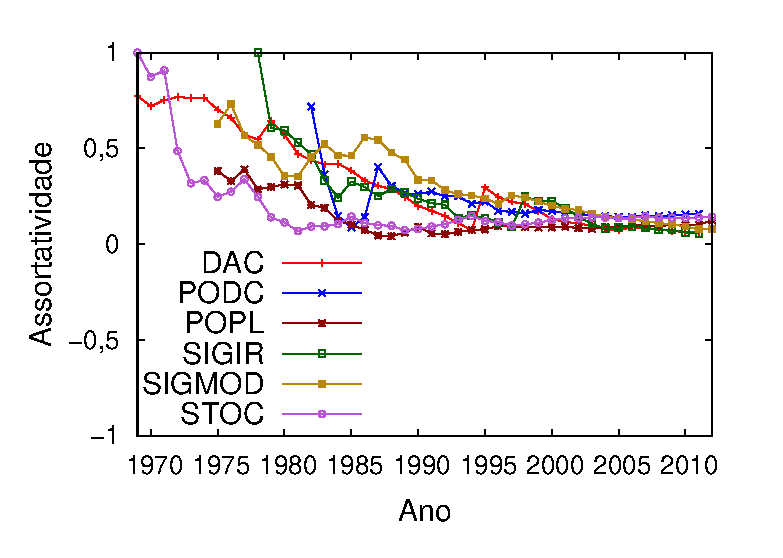
\includegraphics[scale=.6]{../graficos/sigs_metricas_acumuladas_1_em_1_ano/pt_BR/assortatividade_grupo_temporal_web.eps}
  }%
  \subfloat[Assortatividade por janela]{%
    \label{fig:assortativity_slide_window}
    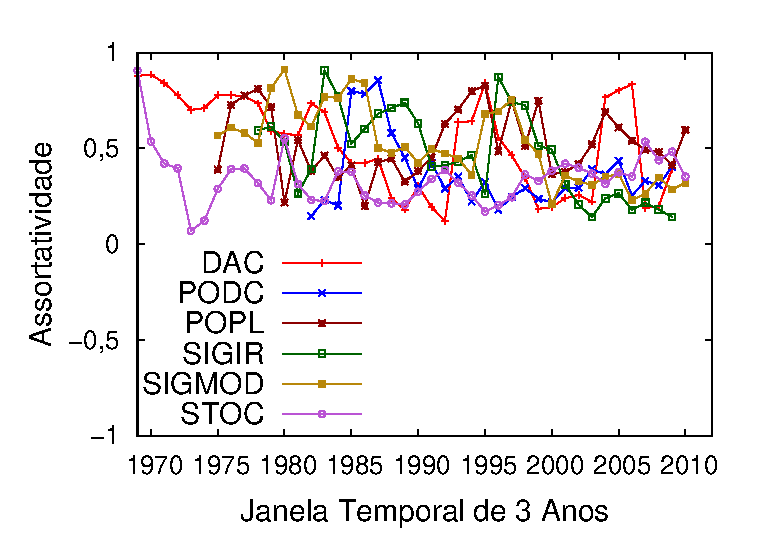
\includegraphics[scale=.6]{../graficos/core_over_time/metricas_tradicionais/pt_BR/assortatividade_slide_window_grupo_temporal_web.eps}
  }%
  \end{center}
  \caption{Assortatividade das comunidades científicas}
  \label{fig:metrics_assortativity}
\end{figure}


\begin{figure}[!htb]
  \begin{center}
  \subfloat[Grau médio final]{%
    \label{fig:average_degree_1_in_1}
    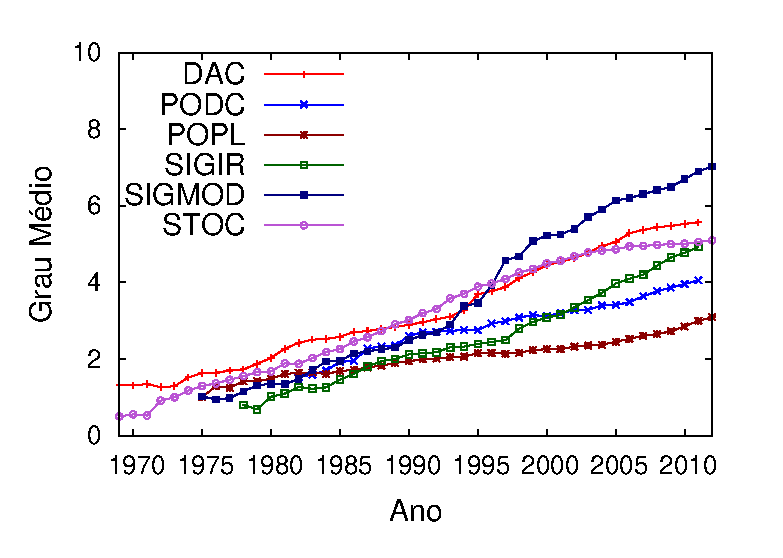
\includegraphics[scale=.6]{../graficos/sigs_metricas_acumuladas_1_em_1_ano/pt_BR/grau_medio_nodos_grupo_temporal_web.eps}
  }%
  \subfloat[Grau médio por janela]{%
    \label{fig:average_degree_slide_window}
    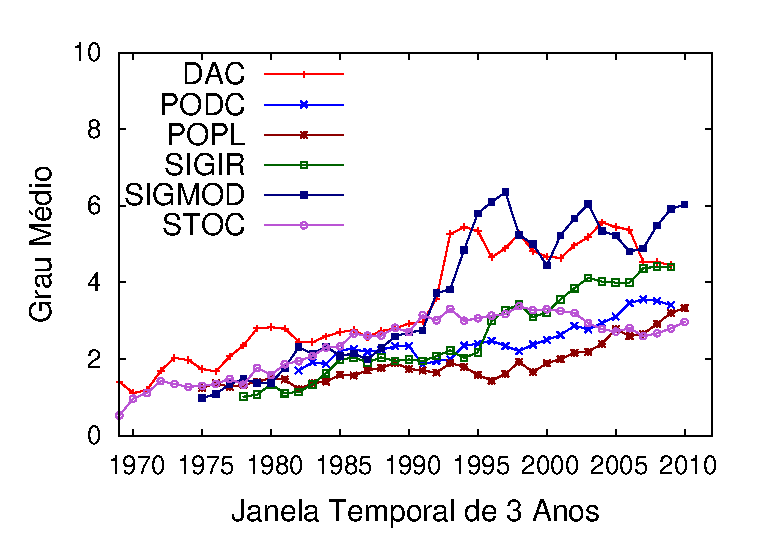
\includegraphics[scale=.6]{../graficos/core_over_time/metricas_tradicionais/pt_BR/grau_medio_nodos_slide_window_grupo_temporal_web.eps}
  }%
  \end{center}
  \caption{Grau médio das comunidades científicas}
  \label{fig:metrics_average_degree}
\end{figure}

% \begin{figure}[!htb]
%   \vspace{-0.2cm}
%   \begin{center}
%   \subfloat[Final Assortativity]{%
%     \label{fig:assortativity_1_in_1}
%     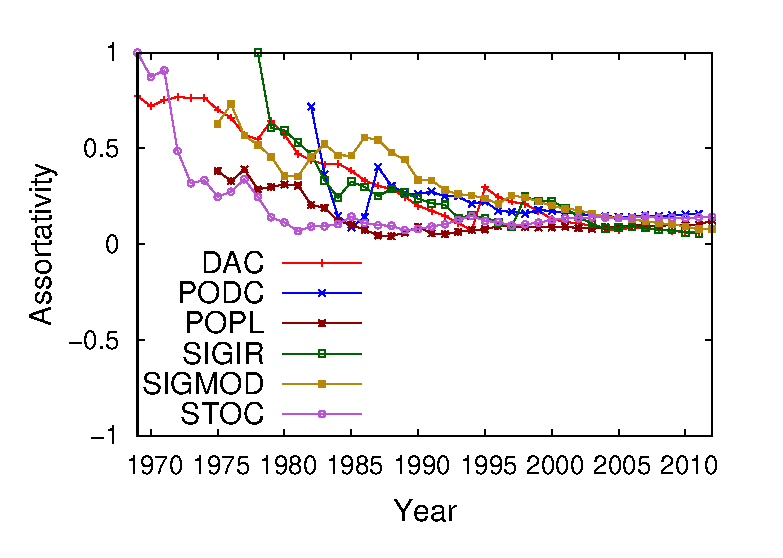
\includegraphics[scale=.33]{../graficos/sigs_metricas_acumuladas_1_em_1_ano/en_US/assortatividade_grupo_temporal_web.eps}
%   }%
%   \subfloat[Assortativity per Window]{%
%     \label{fig:assortativity_slide_window}
%     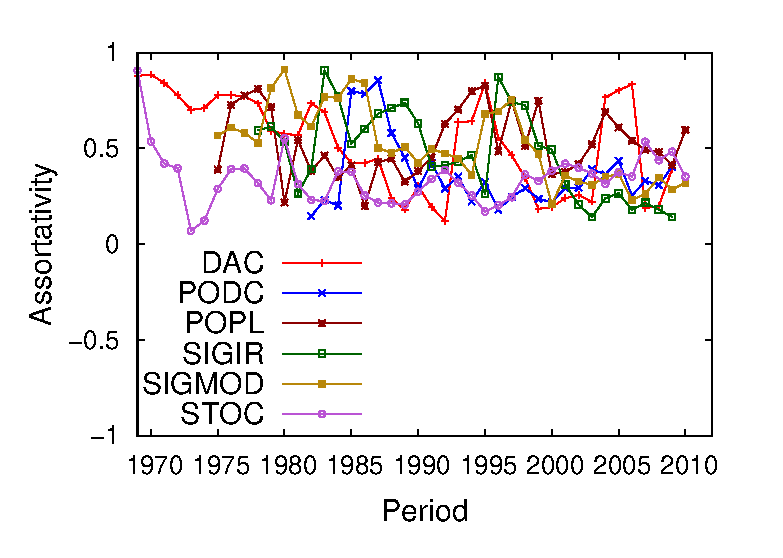
\includegraphics[scale=.33]{../graficos/core_over_time/metricas_tradicionais/en_US/assortatividade_slide_window_grupo_temporal_web.eps}
%   }%
%   \\
%   \subfloat[Final ASP]{%
%     \label{fig:average_shortest_path_1_in_1}
%     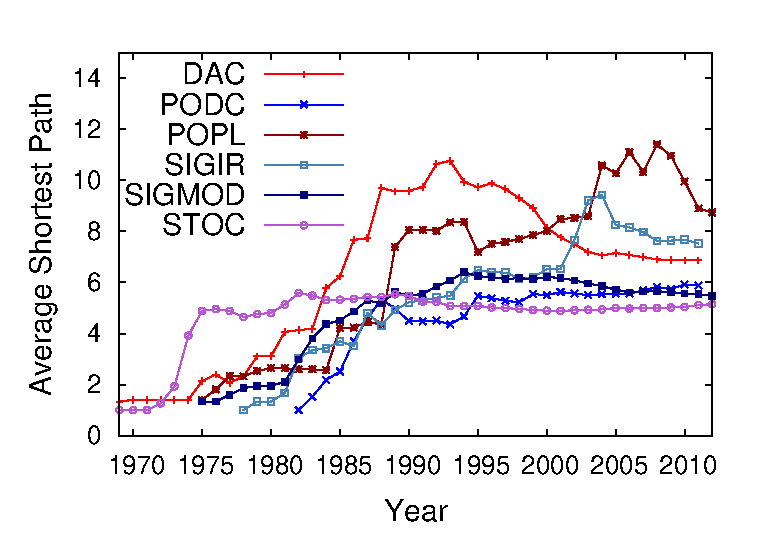
\includegraphics[scale=.33]{../graficos/sigs_metricas_acumuladas_1_em_1_ano/en_US/caminho_minimo_medio_grupo_temporal_web.eps}
%   }%
%   \subfloat[ASP per Window]{%
%     \label{fig:average_shortest_path_slide_window}
%     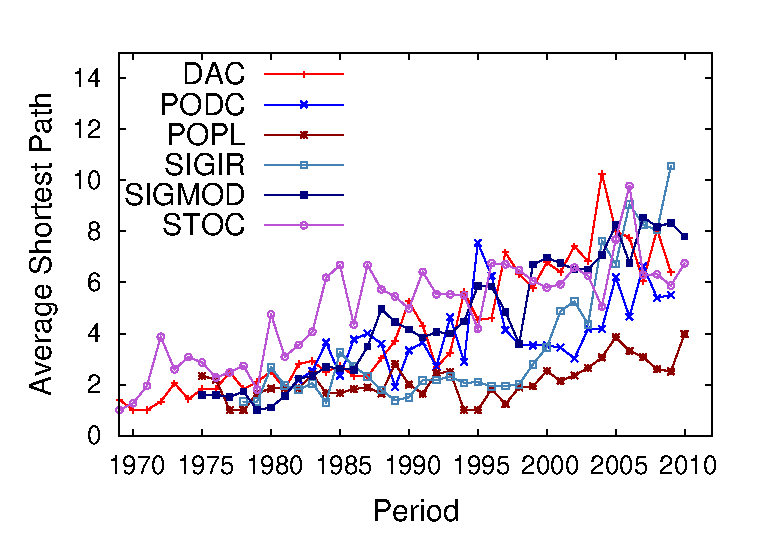
\includegraphics[scale=.33]{../graficos/core_over_time/metricas_tradicionais/en_US/caminho_minimo_medio_slide_window_grupo_temporal_web.eps}
%   }%
%   \\
%   \subfloat[Final CC]{%
%     \label{fig:clustering_coefficient_1_in_1}
%     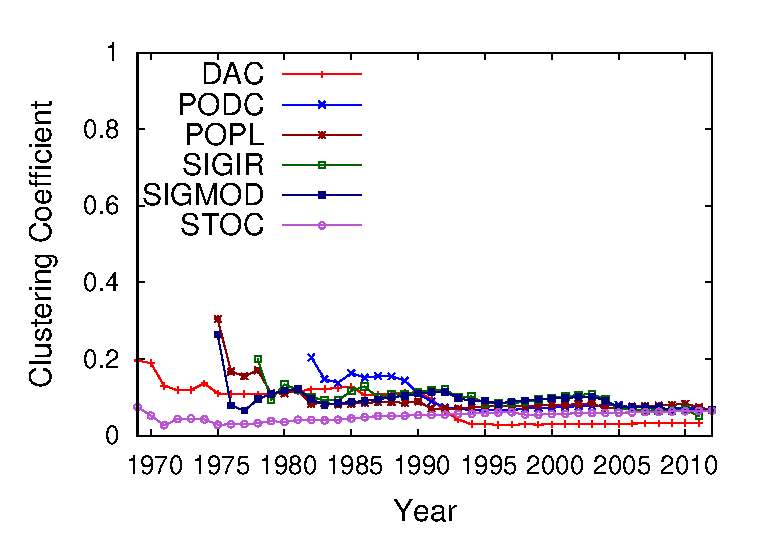
\includegraphics[scale=.33]{../graficos/sigs_metricas_acumuladas_1_em_1_ano/en_US/coeficiente_agrupamento_grupo_temporal_web.eps}
%   }%
%   \subfloat[CC per Window]{%
%     \label{fig:clustering_coefficient_slide_window}
%     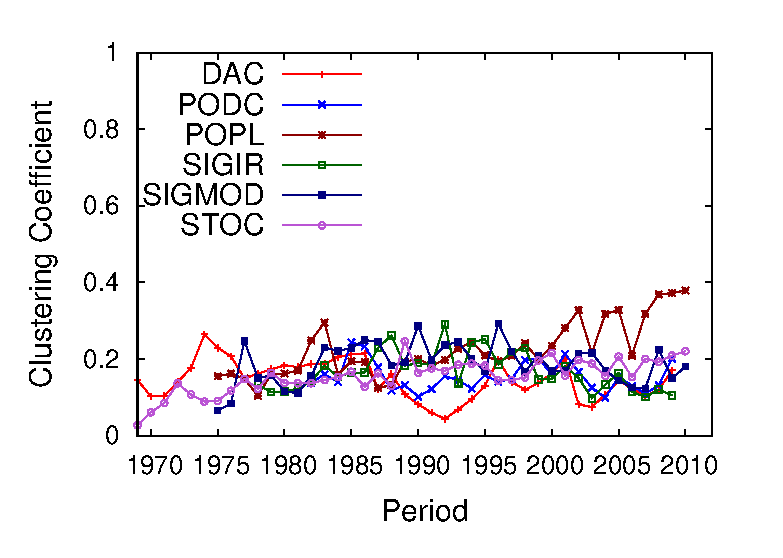
\includegraphics[scale=.33]{../graficos/core_over_time/metricas_tradicionais/en_US/coeficiente_agrupamento_slide_window_grupo_temporal_web.eps}
%   }%
%   \\
%   \subfloat[Final Largest WCC]{%
%     \label{fig:largest_connected_component_1_in_1}
%     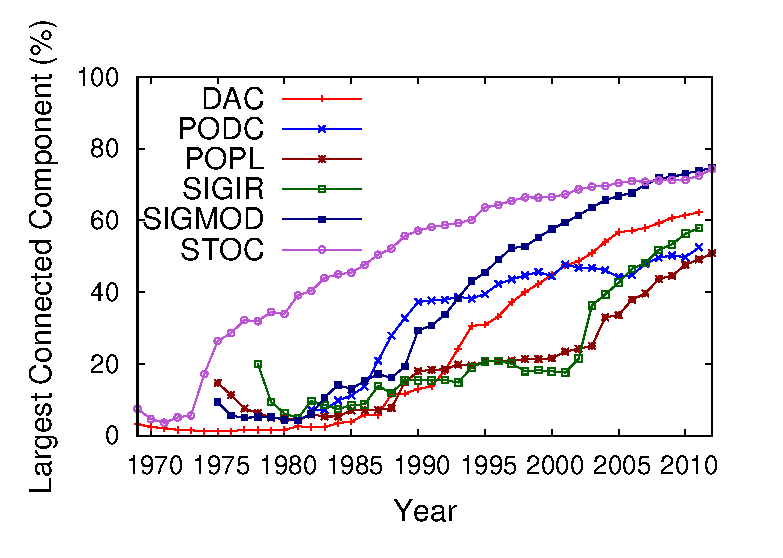
\includegraphics[scale=.33]{../graficos/sigs_metricas_acumuladas_1_em_1_ano/en_US/porcentagem_maior_componente_grupo_temporal_web.eps}
%   }%
%   \subfloat[Largest WCC per Window]{%
%     \label{fig:largest_connected_component_slide_window}
%     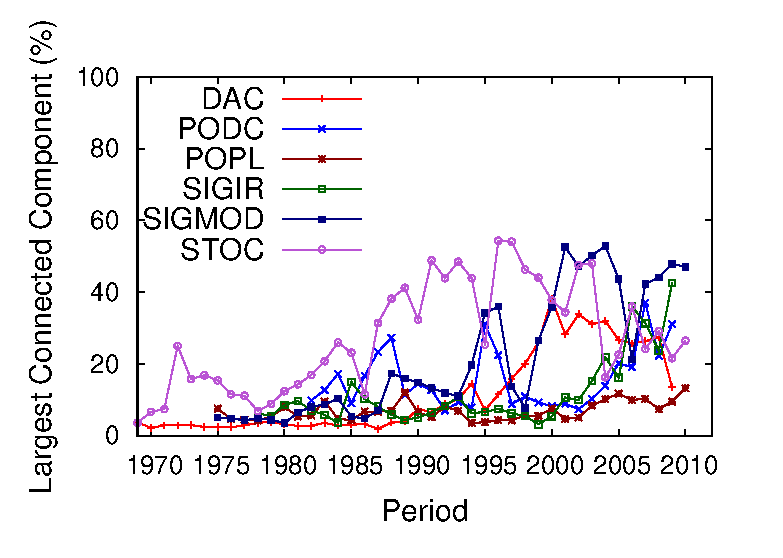
\includegraphics[scale=.33]{../graficos/core_over_time/metricas_tradicionais/en_US/porcentagem_maior_componente_slide_window_grupo_temporal_web.eps}
%   }%
%   \\
%   \subfloat[Final Average Degree]{%
%     \label{fig:average_degree_1_in_1}
%     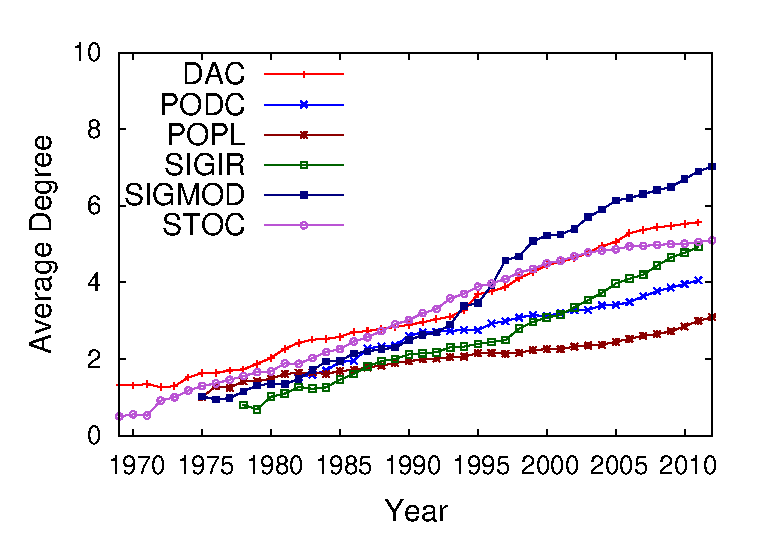
\includegraphics[scale=.33]{../graficos/sigs_metricas_acumuladas_1_em_1_ano/en_US/grau_medio_nodos_grupo_temporal_web.eps}
%   }%
%   \subfloat[Avg. Degree per Window]{%
%     \label{fig:average_degree_slide_window}
%     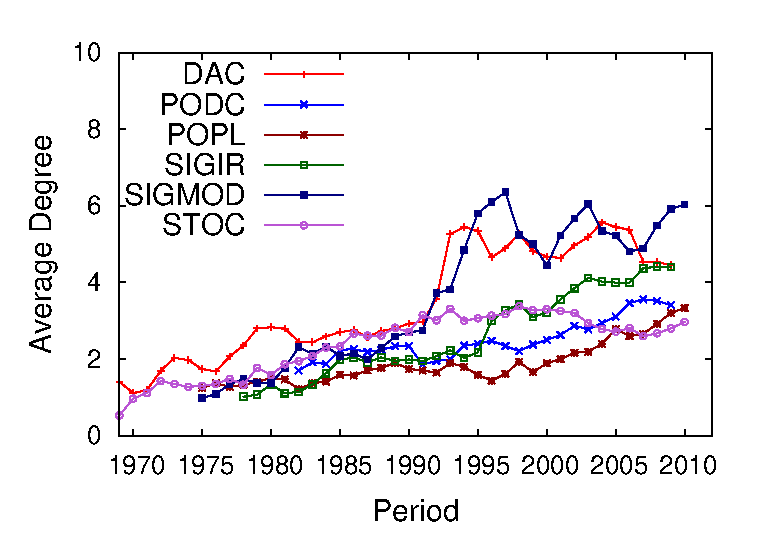
\includegraphics[scale=.33]{../graficos/core_over_time/metricas_tradicionais/en_US/grau_medio_nodos_slide_window_grupo_temporal_web.eps}
%   }%
%   \end{center}
%   \vspace{-0.5cm}
%   \caption{Network evolution metrics for scientific communities}
%   \vspace{-0.5cm}
%   \label{fig:metrics}
% \end{figure}

Notamos a partir da Figura~\ref{fig:metrics_largest_connected_component} que o maior CFC tende a aumentar largamente em função do 
tempo. Isto sugere que na fase inicial, as comunidades científicas são formadas por vários grupos de pesquisa pequenos 
e segregados. Com o tempo, alguns pesquisadores (e.g., estudantes) deixam suas instituições e começam a colaborar com outros 
grupos de pesquisa. Além disso, como a comunidade evolui, líderes de grupos de pesquisa tendem a colaborar com outros colegas 
da mesma comunidade. Assim, com o tempo, pesquisadores de diferentes grupos tendem a colaborar e aumentar o tamanho do maior 
CFC. Como consequência, o caminho mínimo médio, calculado apenas sobre o maior CFC, tende a aumentar, 
se tornando estável em torno de valores semelhantes aos de redes de mundo pequeno (ou seja, caminhos que contenham de 4 a 10 
arestas)~\citep{Mislove2007, Backstrom2012}, conforme Figura~\ref{fig:metrics_average_shortest}. 
Também podemos observar na Figura~\ref{fig:metrics_clustering_coefficient} que o coeficiente de agrupamento médio tende a valores 
entre 0,1 e 0,2, sugerindo que os coautores de um pesquisador têm entre 10\% e 20\% de chance de serem conectados entre 
si. Esses valores tendem a diminuir ligeiramente ao longo do tempo, tal como pequenos componentes tendem a se
conectar para formarem componentes maiores, reduzindo a média do coeficiente de agrupamento. Quando se trata de assortatividade, 
observamos na Figura~\ref{fig:metrics_assortativity} que esta medida tende a 0, mas ainda assim é positiva. Isso significa que 
há uma ligeira tendência nessas comunidades de nodos se conectarem com outros de grau similar. Um valor positivo para a
assortatividade é uma característica típica das redes sociológicas~\citep{Newman2003}. Finalmente, podemos observar na 
Figura~\ref{fig:metrics_average_degree} que o grau médio dos nodos tende a aumentar ao longo do tempo, mesmo com a assortatividade
tendendo a 0. Isto pode indicar uma renovação, em que novos pesquisadores se juntam à rede através de pesquisadores mais experientes,
por exemplo, estudantes com seus orientadores.

% We note from Figure~\ref{fig:metrics} that the largest WCC tend to largely increase as a function of time. This suggests that at early
% stages, scientific communities are formed by several small and segregated research groups. With time, some researchers (e.g., students) leave their institutions and begin collaborations
% with other research groups. Additionally, as the community evolves, heads of  research groups tend to collaborate with other peers of the same community. Thus, with time, researchers
% from different groups tend to collaborate and increase the size of the largest WCC. As a consequence, the average shortest path, computed only on the largest
% WCC, tends to increase, becoming stable around typical small-world values (i.e., from 4 to 10 hops)~\cite{mislove-2007-socialnetworks,fourdegrees_facebook}.  We can
% also note that the average clustering coefficient tends to values between 0.1 and 0.2, thus suggesting that the coauthors of a researcher have 10\% to 20\% of chance to be connected
% among themselves. These values tend to slightly diminish over time, as small components tend to connect to form larger components reducing the average clustering coefficient
% value.  When it comes to assortativity, we see that this measure tends to 0, but it is still positive. This means that there is a slight tendency in these communities of nodes to
% connect with others with similar degree.  A positive value for assortativity is a typical characteristic of sociological networks~\cite{Newman2003}.
% \redcomment{pare aqui}

Em geral, podemos observar que as comunidades científicas têm características de evolução semelhantes e que essas propriedades 
são dinâmicas, mudando ao longo do tempo. Mais importante ainda, nossas observações sugerem que um pequeno grupo de 
pesquisadores que fazem parte do núcleo são responsáveis por criar caminhos entre grupos de pesquisa menores e mais 
conectados. A fim de investigar melhor os pesquisadores que fazem parte do núcleo, na próxima seção comparamos membros e 
não membros dos núcleos das comunidades.

% In general, we can note that scientific communities have similar evolving characteristics and these properties are dynamic as they change over time.  More important, our
% observations suggest that a small set of core researchers are responsible for the social clue that creates the paths among smaller and more connected research groups. In order to 
% further investigate these core researchers in the next subsection we contrast members and non-members of the community core. 


%%%%%%%%%%%%%%%%%%%%%%%%%%%%%%%%%%%
\section{Caracterização dos Núcleos das Comunidades}\label{sub:vs}
%%%%%%%%%%%%%%%%%%%%%%%%%%%%%%%%%%%

\textit{Até que ponto as propriedades dos membros do núcleo diferem dos demais membros das comunidades?} Para responder a essa 
pergunta, calculamos as propriedades de rede para os membros e não membros dos núcleos das comunidades. Consideramos 
a análise de janelas de tempo para compreender as variações que essas duas classes podem ter na medida global. 
A Figura~\ref{fig:metrics_comparing_core_community} mostra o grau médio e o coeficiente de agrupamento médio calculados para 
membros e não membros do núcleo da comunidade SIGMOD, os resultados obtidos para as demais comunidades podem ser encontrados 
no Apêndice~\ref{apendice:comparacao_nucleo}, sendo que nossas observações são válidas para todas elas. Além disso, 
também medimos a fração de membros do núcleo, bem como dos não membros que estão no maior CFC e calculamos 
o \textit{betweenness} médio de cada um desses grupos de membros.

% \textit{To what extend the properties of the community core differ from the rest of the community?}  To answer this question, we compute node 
% network properties for members and non-members of the community
% core. We consider the time window analysis to understand the variations that these two classes might have in the global measure.
% Figure~\ref{fig:metrics_comparing_core_community} shows the average degree and the average clustering coefficient computed by the members and non-members of the SIGMOD 
% community core. Additionally, we also measure the fraction of community core members as well as non-members that are in the largest WCC and compute the average betweenness of
% each of these group of members. 

\begin{figure}[!htb]
  \begin{center}
  \subfloat[Coeficiente de agrupamento]{%
    \label{fig:core_com_sigmod_clustering_coefficient}
    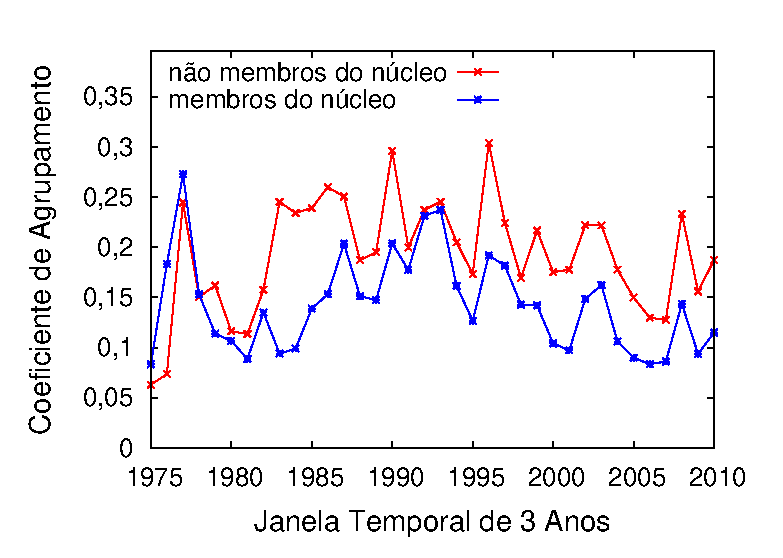
\includegraphics[scale=.6]{../graficos/core_over_time/core_community/pt_BR/sigmod_janela_3_core_coeficiente_agrupamento.eps}
  }
  \subfloat[Grau médio]{%
    \label{fig:core_com_sigmod_average_degree}
    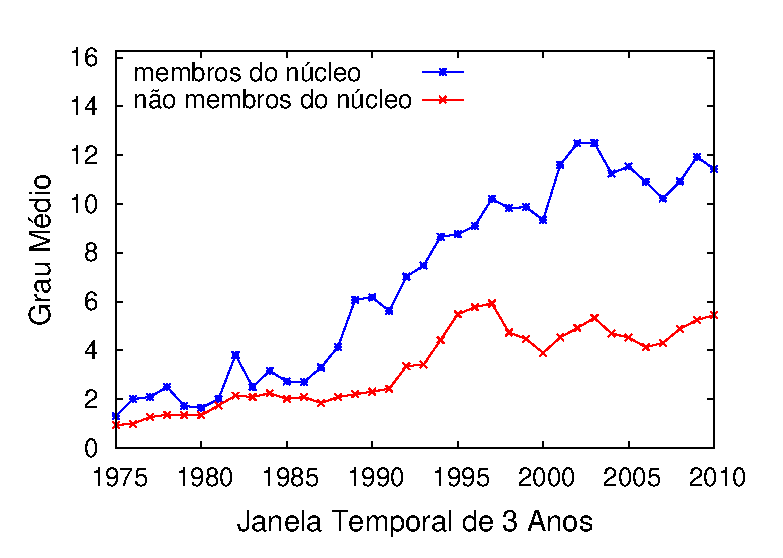
\includegraphics[scale=.6]{../graficos/core_over_time/core_community/pt_BR/sigmod_janela_3_core_grau_medio_nodos.eps}
  }
  \\
  \subfloat[Maior CFC]{%
    \label{fig:core_com_sigmod_largest_connected_component}
    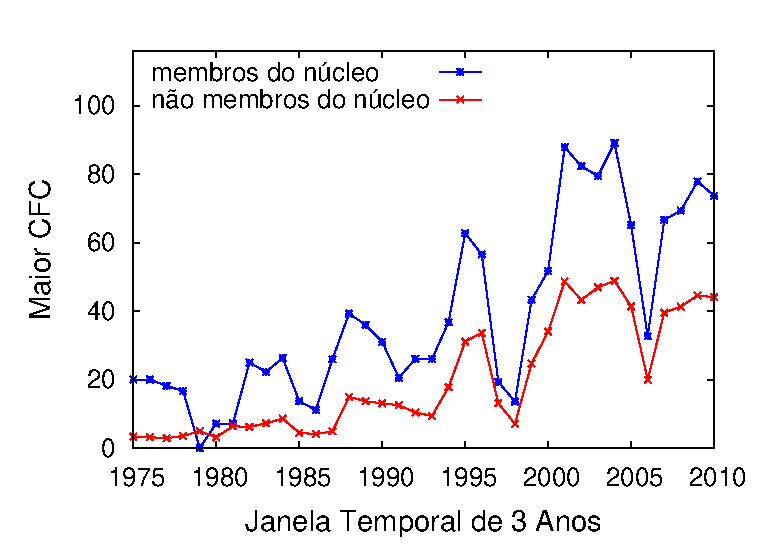
\includegraphics[scale=.6]{../graficos/core_over_time/core_community/pt_BR/sigmod_janela_3_core_maior_componente_conectado.eps}
  }
  \subfloat[\textit{Betweenness} médio]{%
    \label{fig:core_com_sigmod_betweenness}
    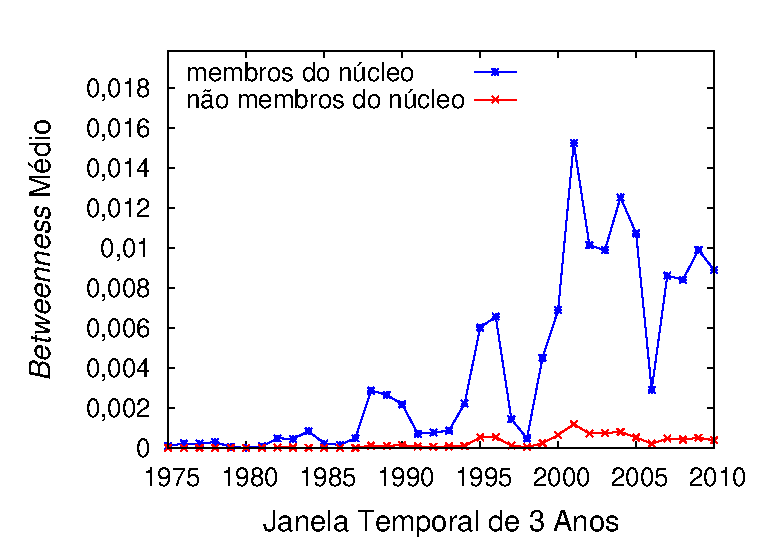
\includegraphics[scale=.6]{../graficos/core_over_time/core_community/pt_BR/sigmod_janela_3_core_betweenness.eps}
  }
  \end{center}
  \caption{Propriedades da comunidade SIGMOD para os membros e não membros do núcleo}
  \label{fig:metrics_comparing_core_community}
\end{figure}

% \begin{figure}[!htpb]
%   \begin{center}
%   \subfloat[Clustering Coefficient]{%
%     \label{fig:core_com_sigmod_clustering_coefficient}
%     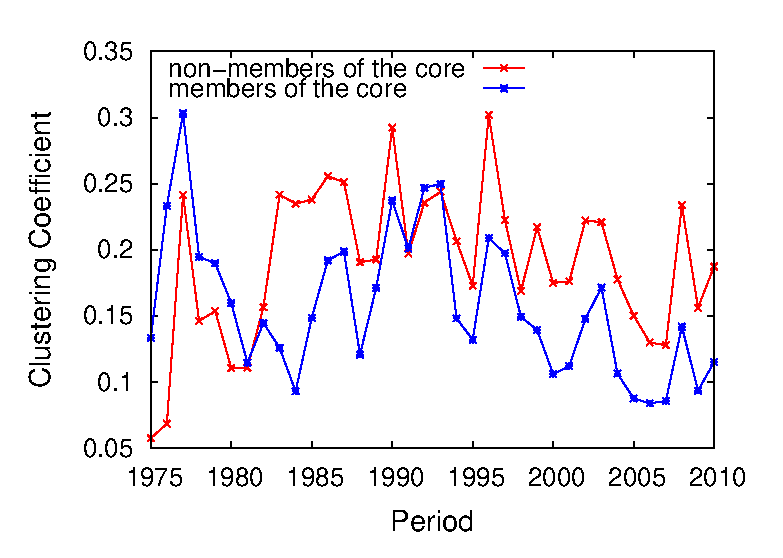
\includegraphics[scale=.31]{../graficos/core_over_time/core_community/en_US/sigmod_janela_3_core_coeficiente_agrupamento.eps}
%   }
%   \subfloat[Avg. Degree]{%
%     \label{fig:core_com_sigmod_average_degree}
%     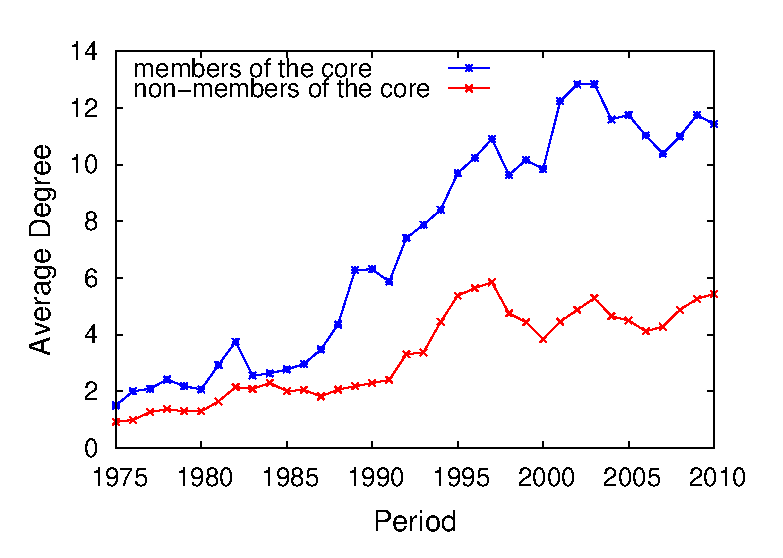
\includegraphics[scale=.31]{../graficos/core_over_time/core_community/en_US/sigmod_janela_3_core_grau_medio_nodos.eps}
%   }
%   \\
%   \subfloat[Largest WCC]{%
%     \label{fig:core_com_sigmod_largest_connected_component}
%     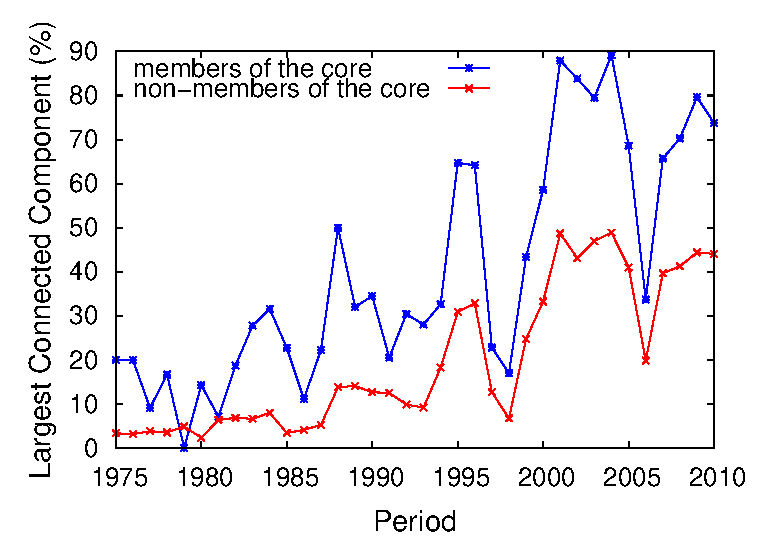
\includegraphics[scale=.31]{../graficos/core_over_time/core_community/en_US/sigmod_janela_3_core_maior_componente_conectado.eps}
%   }
%   \subfloat[Avg. Betweenness]{%
%     \label{fig:core_com_sigmod_betweenness}
%     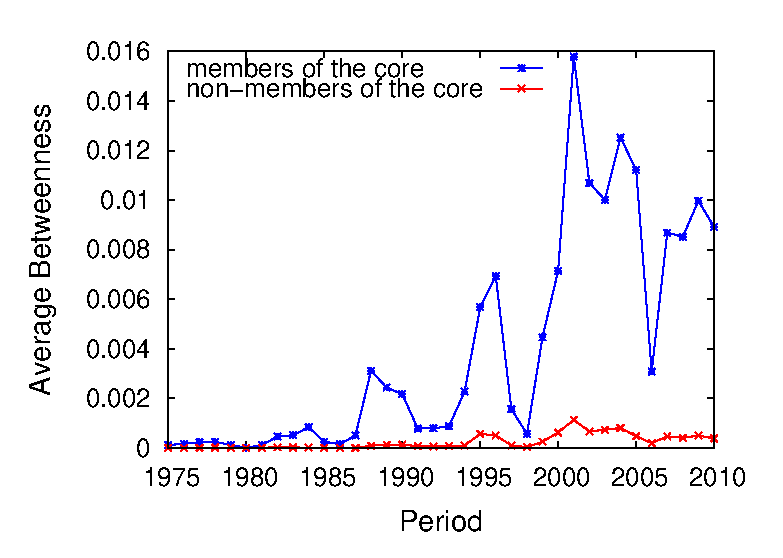
\includegraphics[scale=.31]{../graficos/core_over_time/core_community/en_US/sigmod_janela_3_core_betweenness.eps}
%   }
%   \end{center}
%   \vspace{-0.5cm}
%   \caption{SIGMOD network properties for members and non-members of the core}
%   \label{fig:metrics_comparing_core_community}
% \end{figure}

Podemos fazer observações importantes a partir dessas análises. Primeiro, podemos observar que o grau médio dos membros 
dos núcleos é consideravelmente maior em comparação com o dos não membros, que tendem a estabelecer mais e mais 
conexões em função do tempo. No entanto, o coeficiente de agrupamento dos membros do núcleo tendem a ser 
ligeiramente menor quando comparados com o dos não membros, o que significa que eles podem atuar como \textit{hubs}, conectando 
diferentes grupos com pequenas interseções. Ao analisar a fração de membros do núcleo que fazem parte do maior 
CFC, podemos notar que é muito maior do que a fração de não membros, sugerindo que eles podem estar conectando componentes 
menores. Confirmamos essas observações, analisando a centralidade desses grupos de pesquisadores através da métrica \textit{betweenness}. 
Podemos notar que o \textit{betweenness} médio do núcleo da comunidade é muito maior, o que significa que um maior número de caminhos mais 
curtos incluem esses nodos.

% We can make key observations
% from theses analysis. First, we can note that the average degree of the members of the community core is considerably higher in comparison with non-members, as they tend to establish more and
% more connections as a function of time. However, the clustering coefficient of the members of the community core tend to be slightly smaller in comparison with non-members meaning that they
% might act like hubs, by connecting different groups with small intersection. By analyzing the fraction of members of the community core that are part of the largest
% WCC, we can note that it is much larger than the fraction of non-members, suggesting that they might be connecting smaller components. 
% We confirm these observations by analyzing the betweenness centrality of these groups of researchers. We can note that the average betweenness of the community core is much higher,
% meaning that a higher number of shortest paths include these nodes. 

Na próxima seção investigamos como aspectos dos membros dos núcleos podem impactar a estrutura geral das comunidades.

% Next, we investigate how aspects of the members of a community core can impact on the overall structure of the community.

%%%%%%%%%%%%%%%%%%%%%%%%%%%%%%%%%%%
\section{Impacto dos Membros dos Núcleos na Estrutura Topológica das Comunidades}\label{sub:corr}
%%%%%%%%%%%%%%%%%%%%%%%%%%%%%%%%%%%

Agora analisamos o quanto as variações no núcleo da comunidade afetam a estrutura da rede. Para isso, calculamos 
a média do \textit{CoScore} dos membros de cada comunidade ao longo do tempo. Intuitivamente, essa medida captura a 
prolificidade global e o grau de participação dos membros do núcleo em uma comunidade científica. A Figura~\ref{fig:average_core_score} 
mostra o \textit{CoScore} médio para um conjunto específico de comunidades em função do tempo. Nossa análise abrange todas as comunidades, podendo os gráficos das demais 
serem observados no Apêndice~\ref{apendice:evolucao_pontuacao_nucleo}. Plotamos em duas figuras distintas para 
facilitar a visualização. Podemos observar em todas as comunidades que, apesar de pequenas quedas, de forma geral o valor aumenta 
ao longo do tempo sofrendo variações. Podemos especular inúmeros fatores que são capazes de explicar essas pequenas variações, incluindo a expansão 
ou redução do número de artigos publicados, a ascensão e queda de temas com capacidade de atrair pesquisadores ou a perda de 
membros importantes do núcleo, membros envolvidos na organização de outras conferências, etc. No entanto, desconsiderando o que 
causou essas variações, queremos investigar se tais variações podem impactar diretamente a estrutura da rede.

% We now examine to what extent the community core fluctuations affect the network structure.  To that end, we compute the average core score of the members of each community over
% time. Intuitively, this measure captures the overall prolificness and involvement of the core members of a scientific community. Figure~\ref{fig:average_core_score} shows this value
% for a set of communities as a function of time. We plot it in two separate figures to facilitate visualization. We can note that all communities experimented rises and falls along
% its life time, indicating strong variations in the core score values of the core members. We can speculate innumerous factors that are able to explain such variations,
% including expansion or reduction in the number of published papers, raise and fall of hot topics with ability to attract or loose important core members, members involved in the
% conference organization, etc. However, disregarding what caused these variations, we want to investigate if such variations can directly impact the network structure.

\begin{figure}[!htb]
  \begin{center}
    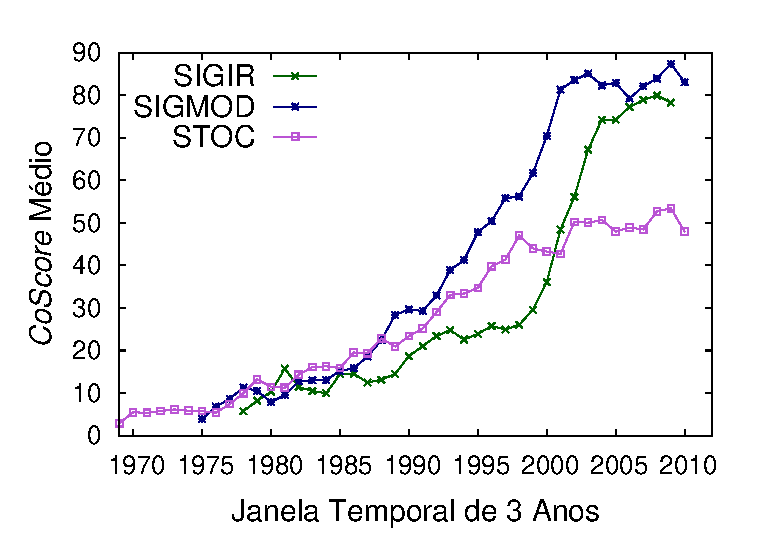
\includegraphics[scale=.6]{../graficos/average_core_score/pt_BR/average_core_score_slide_window_grupo_1_temporal_web.eps}
    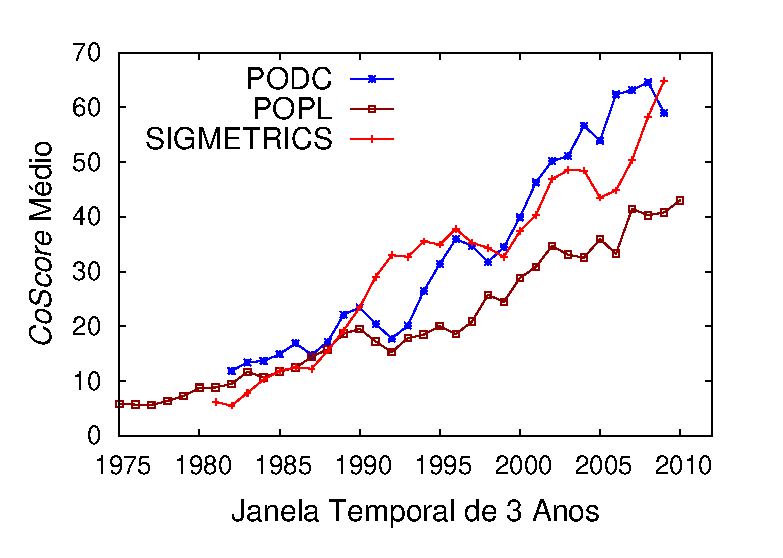
\includegraphics[scale=.6]{../graficos/average_core_score/pt_BR/average_core_score_slide_window_grupo_2_temporal_web.eps}
  \end{center}
  \caption{\textit{CoScore} médio das comunidades científicas}
  \label{fig:average_core_score}
\end{figure}

% \begin{figure}[!htb]
%   \begin{center}
%     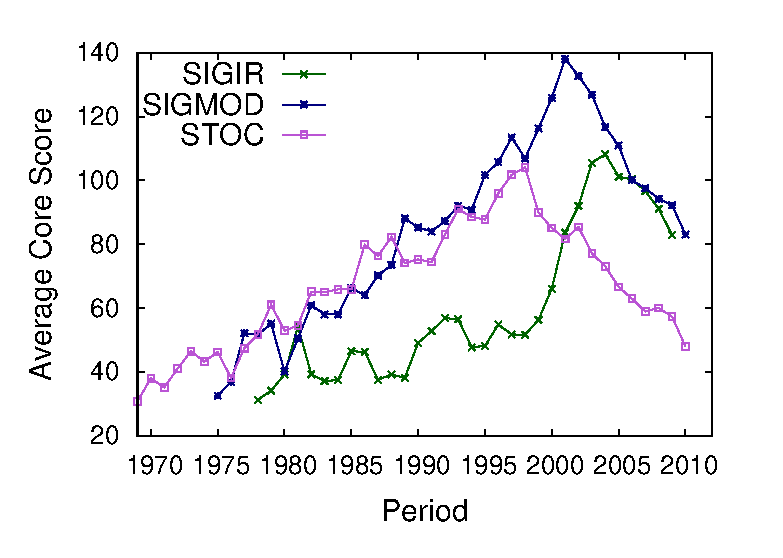
\includegraphics[scale=.325]{../graficos/average_core_score/en_US/average_core_score_slide_window_grupo_1_temporal_web.eps}
%     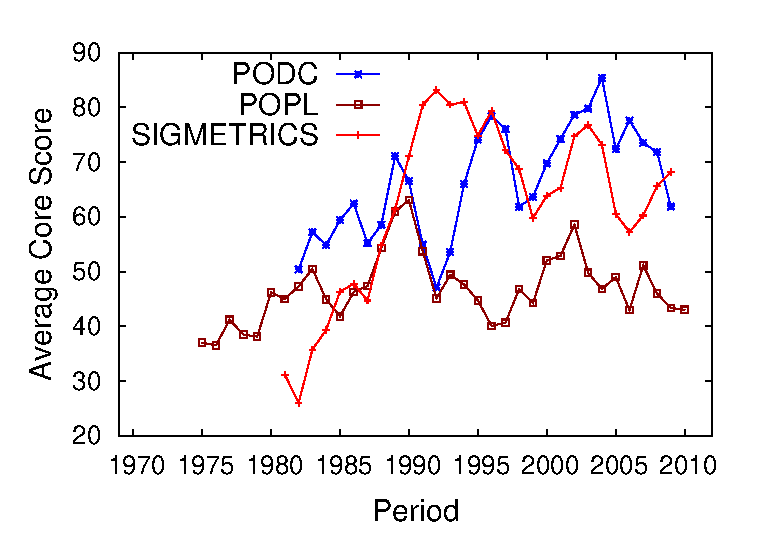
\includegraphics[scale=.325]{../graficos/average_core_score/en_US/average_core_score_slide_window_grupo_2_temporal_web.eps}
%   \end{center}
%   \vspace{-0.5cm}
%   \caption{Avg. core score of scientific communities}
%   \vspace{-0.5cm}
%   \label{fig:average_core_score}
% \end{figure}

Nossa abordagem para investigar esta questão consiste em calcular o coeficiente de correlação de Pearson entre a média do
\textit{CoScore} e as métricas de redes para cada comunidade. A Tabela~\ref{tab:correlation_metrics} apresenta esses valores.

% Our approach to investigate this issue consists of computing the Pearson's correlation coefficient between the average core score of each scientific community and a number of
% network metrics for that community. Table~\ref{tab:correlation_metrics} presents these values.

\begin{table}[!htbp]
\centering
\caption{Correlação entre a média do \textit{CoScore} e as métricas de redes}
\label{tab:correlation_metrics}
{\tiny
\begin{tabular}{|l|c|c|c|c|c|c|} \hline
\textbf{Comunidade} & \textbf{Diâmetro} & \textbf{C. Mín. Méd.} & \textbf{Coef. Agrup.} & \textbf{Assort.} & \textbf{Maior CFC} & \textbf{Grau Méd.} \\ \hline
CCS & 0,81 & 0,78 & -0,36 & -0,67 & 0,49 & 0,88 \\ \hline
CHI & 0,91 & 0,91 & -0,82 & -0,84 & 0,95 & 0,85 \\ \hline
CIKM & 0,79 & 0,79 & -0,53 & -0,82 & 0,65 & 0,97 \\ \hline
DAC & 0,94 & 0,94 & -0,41 & -0,52 & 0,90 & 0,90 \\ \hline
HSCC & 0,38 & 0,65 & -0,72 & -0,34 & 0,80 & 0,58 \\ \hline
ICSE & 0,73 & 0,75 & -0,39 & -0,72 & 0,44 & 0,98 \\ \hline
ISCA & 0,57 & 0,58 & 0,62 & -0,33 & 0,67 & 0,85 \\ \hline
KDD & 0,61 & 0,69 & -0,11 & -0,94 & 0,76 & 0,74 \\ \hline
MICRO & 0,51 & 0,48 & 0,49 & -0,23 & 0,38 & 0,86 \\ \hline
MM & 0,89 & 0,88 & -0,89 & -0,90 & 0,91 & 0,93 \\ \hline
MOBICOM & 0,73 & 0,81 & 0,15 & -0,41 & 0,81 & 0,80 \\ \hline
PODC & 0,56 & 0,56 & -0,18 & -0,25 & 0,33 & 0,94 \\ \hline
POPL & 0,70 & 0,67 & 0,83 & -0,04 & 0,54 & 0,92 \\ \hline
SAC & 0,76 & 0,77 & 0,06 & -0,60 & -0,57 & 0,76 \\ \hline
SIGCOMM & 0,63 & 0,67 & -0,15 & -0,94 & 0,90 & 0,88 \\ \hline
SIGCSE & 0,78 & 0,71 & -0,18 & -0,40 & 0,92 & 0,93 \\ \hline
SIGDOC & 0,90 & 0,92 & -0,21 & -0,92 & 0,88 & 0,91 \\ \hline
SIGGRAPH & 0,82 & 0,90 & -0,38 & -0,73 & 0,92 & 0,88 \\ \hline
SIGIR & 0,91 & 0,94 & -0,43 & -0,75 & 0,81 & 0,92 \\ \hline
SIGMETRICS & 0,57 & 0,50 & 0,57 & -0,58 & 0,45 & 0,94 \\ \hline
SIGMOD & 0,94 & 0,95 & 0,01 & -0,75 & 0,91 & 0,91 \\ \hline
STOC & 0,73 & 0,78 & 0,70 & 0,03 & 0,62 & 0,84 \\ \hline \hline
{\textbf{Média}} & {\textbf{0,73}} & {\textbf{0,76}} & {\textbf{-0,10}} & {\textbf{-0,58}} & {\textbf{0,66}} & {\textbf{0,87}} \\ \hline
\end{tabular}
}
\end{table}


% \begin{table*}[!htbp]
% \centering
% \caption{Correlation between the average core score of the community cores and the network metrics}
% \label{tab:correlation_metrics}
% {\small
% \begin{tabular}{|l|c|c|c|c|c|c|} \hline
% \textbf{Community} & \textbf{Diameter} & \textbf{Avg. Short P.} & \textbf{Clus. Coef.} & \textbf{Assort.} & \textbf{Larg. WCC} & \textbf{Avg. Deg.} \\ \hline
% CCS & 0.34 & 0.2 & 0.23 & -0.2 & 0.45 & 0.14 \\ \hline
% CHI & 0.75 & 0.79 & -0.62 & -0.74 & 0.76 & 0.77 \\ \hline
% CIKM & 0.56 & 0.56 & -0.52 & -0.67 & 0.39 & 0.87 \\ \hline
% DAC & 0.8 & 0.85 & -0.49 & -0.63 & 0.76 & 0.92 \\ \hline
% HSCC & 0.17 & 0.45 & -0.62 & -0.71 & 0.87 & 0.55 \\ \hline
% ICSE & 0.81 & 0.83 & -0.52 & -0.84 & 0.68 & 0.8 \\ \hline
% ISCA & 0.63 & 0.55 & 0.54 & -0.32 & 0.63 & 0.81  \\ \hline
% ISSAC & 0.05 & 0.01 & -0.25 & -0.43 & -0.07 & 0.21 \\ \hline
% KDD & 0.1 & 0.17 & -0.33 & -0.67 & 0.2 & 0.14\\ \hline
% MICRO & 0.35 & 0.35 & 0.28 & -0.36 & 0.52 & 0.51 \\ \hline
% MOBICOM & -0.04 & 0.11 & 0.13 & -0.65 & 0.23 & -0.09 \\ \hline
% MM & 0.67 & 0.68 & -0.91 & -0.95 & 0.67 & 0.69 \\ \hline
% PODC & 0.4 & 0.42 & -0.23 & -0.2 & 0.13 & 0.68 \\ \hline
% POPL & 0.21 & 0.2 & 0.23 & -0.43 & 0.25 & 0.19 \\ \hline
% SAC & 0.48 & 0.59 & 0.16 & -0.39 & -0.55 & 0.16 \\ \hline
% SIGCOMM & 0.18 & 0.19 & 0.05 & -0.81 & 0.49 & 0.41\\ \hline
% SIGCSE & 0.88 & 0.84 & -0.22 & -0.5 & 0.93 & 0.87 \\ \hline
% SIGDOC & 0.73 & 0.78 & -0.36 & -0.89 & 0.66 & 0.76 \\ \hline
% SIGGRAPH & 0.79 & 0.85 & -0.45 & -0.75 & 0.94 & 0.88 \\ \hline
% SIGIR & 0.83 & 0.85 & -0.42 & -0.77 & 0.7 & 0.89 \\ \hline
% SIGMETRICS & 0.31 & 0.24 & 0.3 & -0.44 & 0.37 & 0.64 \\ \hline
% SIGMOD & 0.78 & 0.81 & 0.27 & -0.61 & 0.77 & 0.87 \\ \hline
% SIGUCCS & 0.38 & -0.22 & 0.53 & -0.13 & 0.51 & 0.7 \\ \hline
% STOC & 0.61 & 0.63 & 0.54 & -0.37 & 0.82 & 0.88\\ \hline \hline
% {\textbf{Average}} & {\textbf{0.49}} & {\textbf{0.49}} & {\textbf{-0.11}} & {\textbf{-0.56}} & {\textbf{0.5}} & {\textbf{0.59}} \\ \hline
% \end{tabular}
% }
% \end{table*}

A partir dessa análise, podemos notar que o diâmetro da rede de uma conferência 
possui uma forte correlação positiva com a média do \textit{CoScore}, sendo este 0,73. Isto significa que, quando a média do
\textit{CoScore} de uma comunidade aumenta ou diminui, o diâmetro tende a seguir a mesma tendência. Isto sugere que os 
membros do núcleo podem conectar componentes menores, criando pontes entre eles, o que contribui para aumentar o diâmetro 
total da rede. Esta conjectura é também suportada pelo alto valor do coeficiente de correlação para o caminho mínimo médio 
(em média 0,76) e o tamanho do maior CFC (em média de 0,66).

% We make key observations from this analysis. First, we can note that the diameter of a conference is positive correlated with the average core score. Although for some communities
% we can see values close to 0 or even negative (e.g., MOBICOM, with -0.04), the average correlation coefficient for all communities is 0.49, which indicates an overall
% positive tendency. This means that when the average core score of a community increases or decreases, the diameter tends to follow the same tendency. This suggests that core 
% members might connect smaller components, creating bridges among them, which contributes to increase the overall diameter. This conjecture is also supported by the high coefficient
% correlation for the average shortest path (on average 0.49) and the size of the largest WCC (on average 0.5).

Em seguida, podemos observar um alto valor positivo do coeficiente de correlação entre a média do \textit{CoScore}
das comunidades e o grau médio da rede. Também, podemos observar uma forte correlação negativa com a 
assortatividade da rede. Isto sugere que um aumento na média do \textit{CoScore} aumenta o conjunto de nodos densamente 
conectados na rede. Entretanto, embora criem caminhos entre os componentes, esses nodos também tendem a se conectar principalmente com nodos de 
menor grau, diminuindo a assortatividade da rede. De fato, um pesquisador sênior tende a ser coautor 
de um grande número de estudantes e jovens pesquisadores, além de manter colaborações com pesquisadores seniores 
de outros grupos.

% Second, on one hand, we can note a highly positive correlation coefficient between the average core score of communities and the average degree of the network and, in the
% other hand, we can 
% observe a strong negative correlation with the assortativeness of the network. This suggests that an increase in the average community core increases the set of highly connected
% nodes in the network. But, although they create paths among components, they tend to connect themselves mostly with nodes of small degree values, decreasing the assortativeness of the
% network. Indeed, a senior researcher might tend to be coauthor of a high number of students and young researchers, but also keep collaborations with other senior researchers from
% other groups.

Finalmente, apesar das variações esperadas, observamos uma tendência clara para a maioria das comunidades em cada uma das 
métricas analisadas (i.e., claras correlações positivas ou negativas para a maioria das comunidades). Isso reforça 
que as nossas observações são válidas para um número significativo de comunidades científicas.

% Finally, despite the expected variations, we note a clear pattern for most of the communities on each of the analyzed metrics (i.e., clear positive or negative correlations for most of the
% communities). This reinforces that our observations hold for a significant number of scientific communities. 


%%%%%%%%%%%%%%%%%%%%%%%%%%%%%%%%%%%
\section{Visualização das Comunidades}
%%%%%%%%%%%%%%%%%%%%%%%%%%%%%%%%%%%

Em complemento a nossas análises, plotamos as comunidades científicas acumulando todos os seus nodos e arestas ao longo 
do tempo. A Figura~\ref{fig:redes} apresenta a plotagem das comunidades SIGMOD, CHI, SAC, e STOC. Cada cor representa um 
componente conectado diferente e o tamanho dos nodos indica o número de vezes que o pesquisador apareceu no núcleo ao 
longo de todo o tempo de vida daquela comunidade. As demais comunidades podem ser observadas no Apêndice~\ref{apendice:redes}. 

A maioria das comunidades apresenta as mesmas características que as comunidades SIGMOD e CHI, possuindo um
grande CFC bem definido chamado de maior CFC, sendo este composto por membros e não membros do núcleo. Observamos 
claramente que um grande número de membros do núcleo se encontra no maior CFC, com algumas pequenas exceções, sendo 
esses membros responsáveis por conectar grupos de outros pesquisadores, conforme apontando em nossas análises anteriormente. 
As comunidades SAC e STOC apresentam um comportamento atípico. A primeira não
possui um grande CFC bem definido. Isto acontece porque essa conferência abrange várias áreas ao longo do tempo, dificultando
assim a fixação dos pesquisadores na comunidade. Outro detalhe sobre a SAC é que ela não possui pesquisadores que participaram 
várias vezes do núcleo, o que indica uma frequente renovação dessa comunidade. Com relação à comunidade STOC, uma conferência 
teórica, é possível verificar o oposto da SAC. A comunidade possui um grande CFC muito bem definido e com grande 
parte dos membros do seu núcleo situada no centro da rede, indicando que os pesquisadores dessa comunidade interagem frequentemente, 
podendo, de certa forma, dificultar a entrada de novos membros.

Por fim, podemos notar que existe um grupo de pesquisadores que persiste no núcleo ao longo da vida de uma dada comunidade e 
a forma como os membros desse núcleo se organizam na rede reforça nossa teoria que esses pesquisadores atuam como pontes 
que interligam grupos de pesquisa dentro da comunidade.


\begin{figure}[!htb]
  \begin{center}
  \subfloat[SIGMOD]{%
    \label{fig:rede_sigmod}
    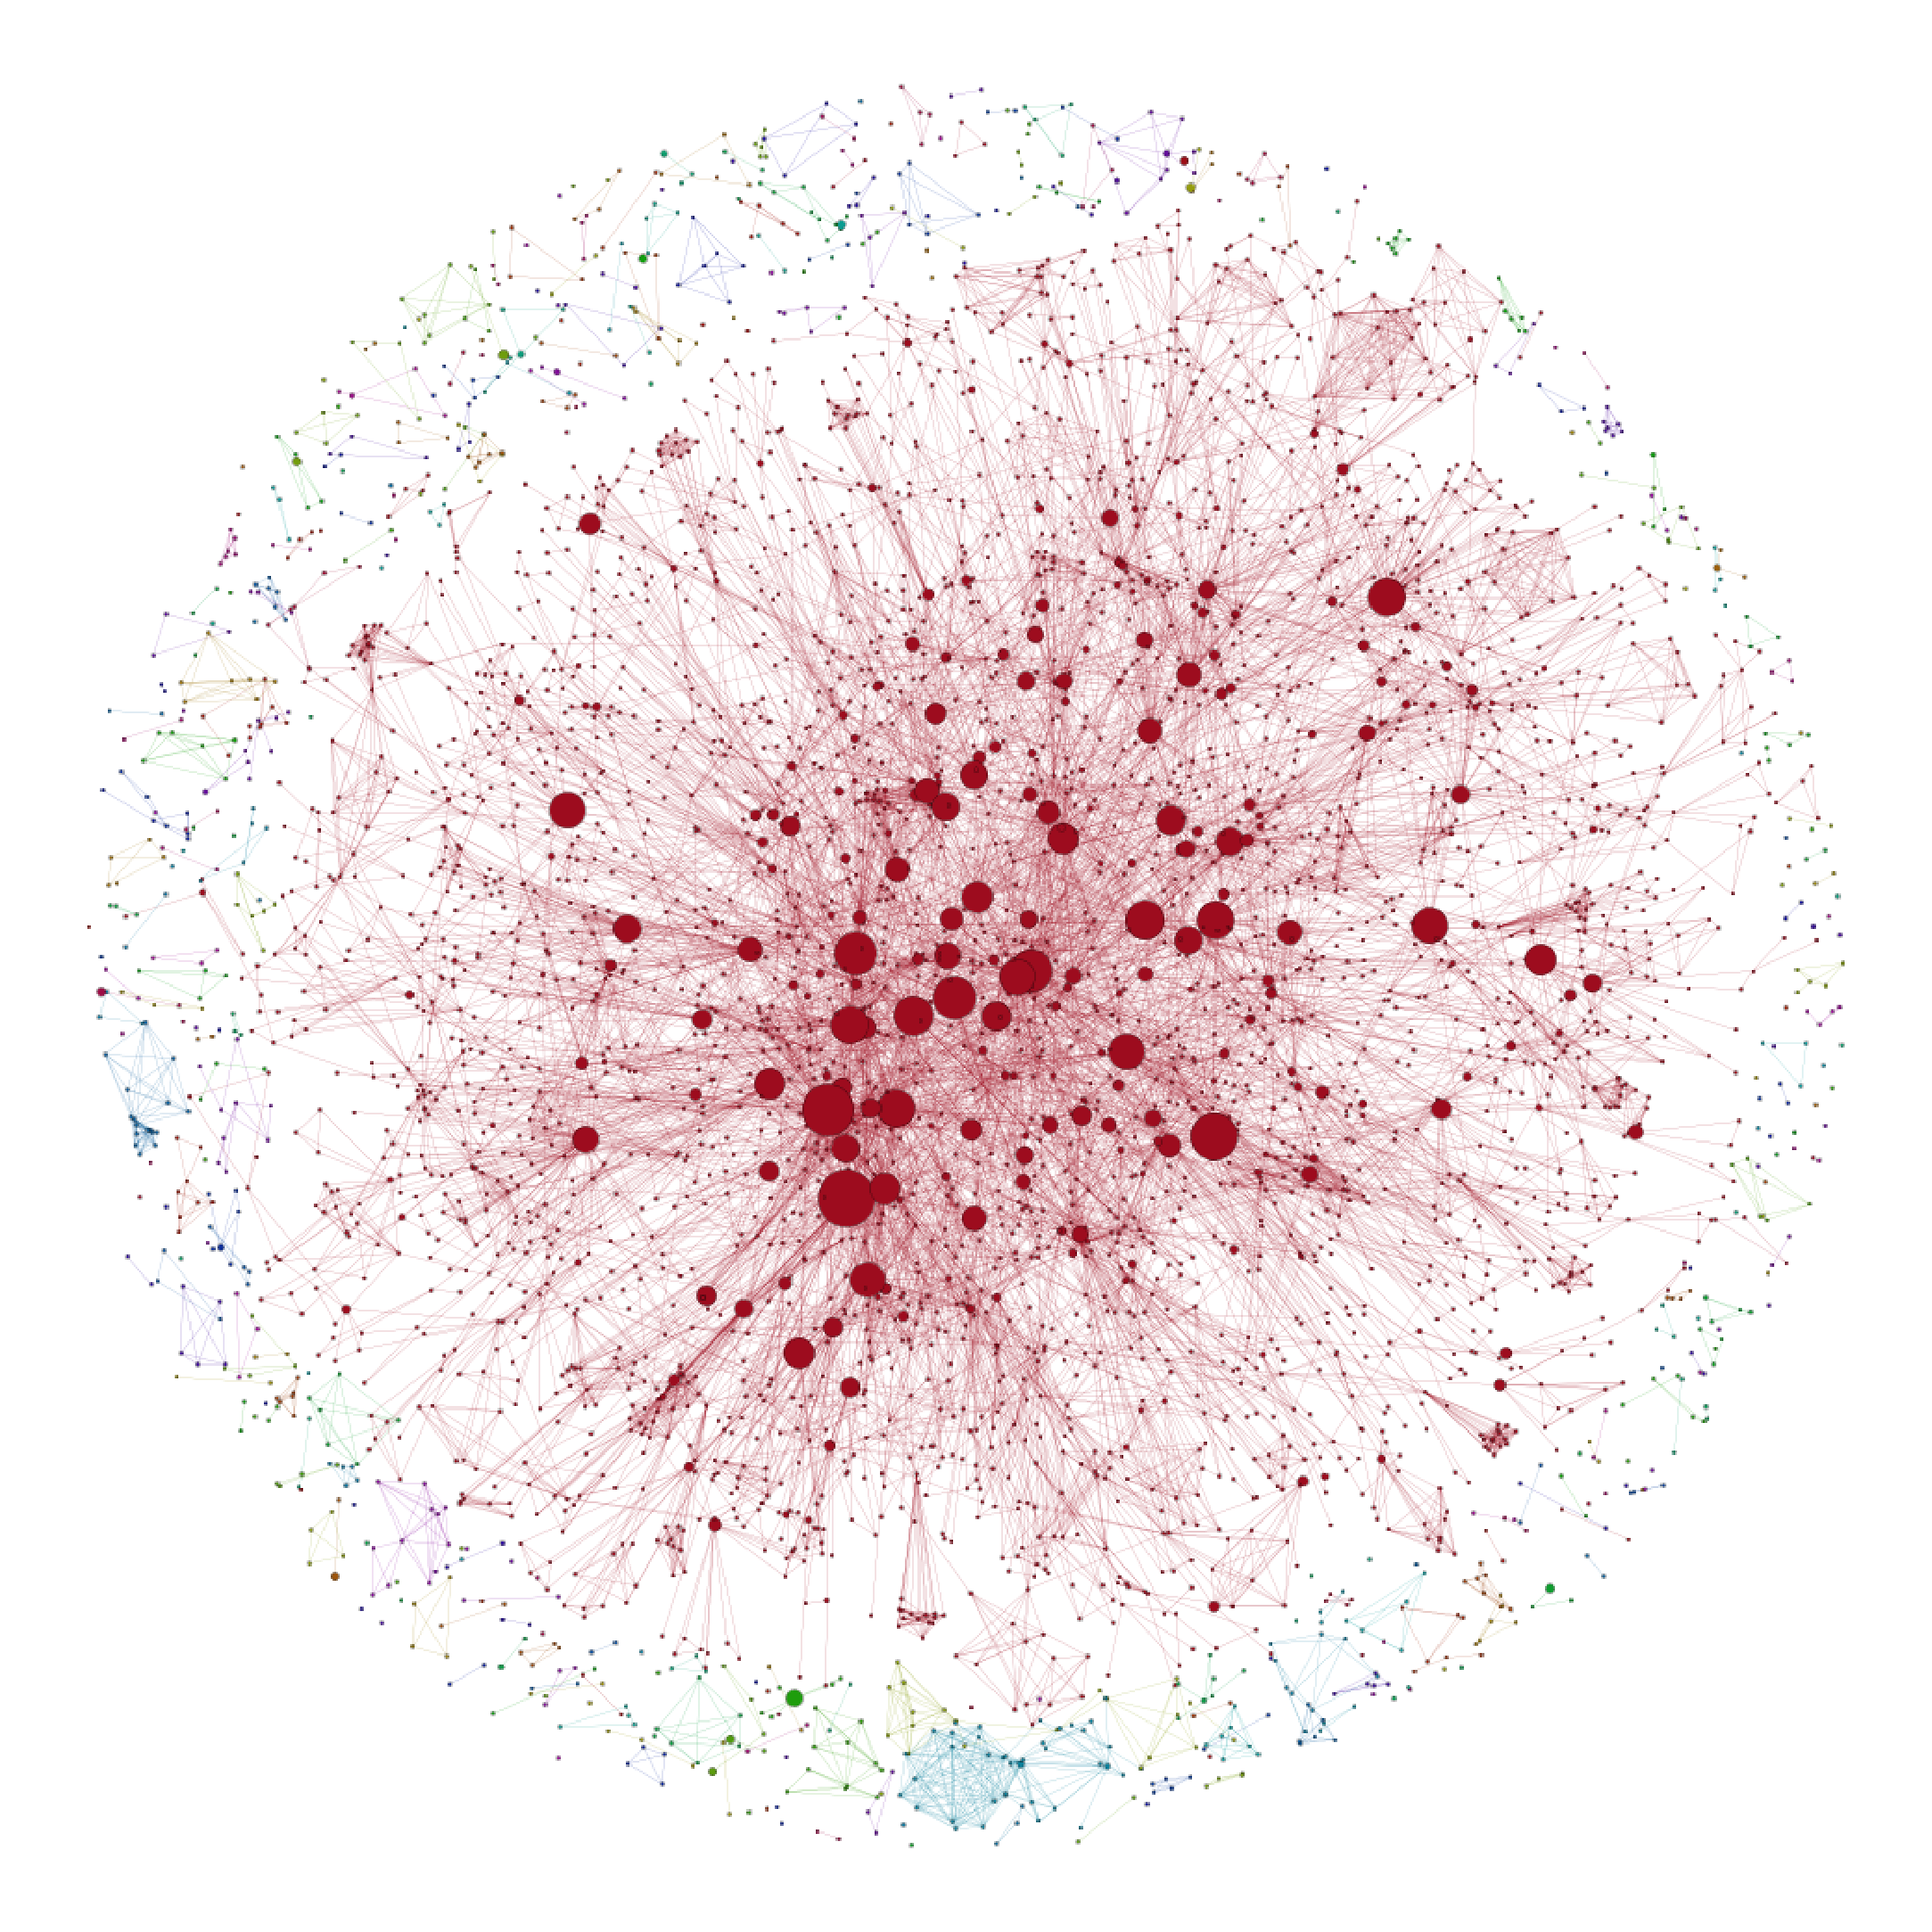
\includegraphics[scale=.21]{../graficos/network/sigmod.eps}
  }%
  \subfloat[CHI]{%
    \label{fig:rede_chi}
    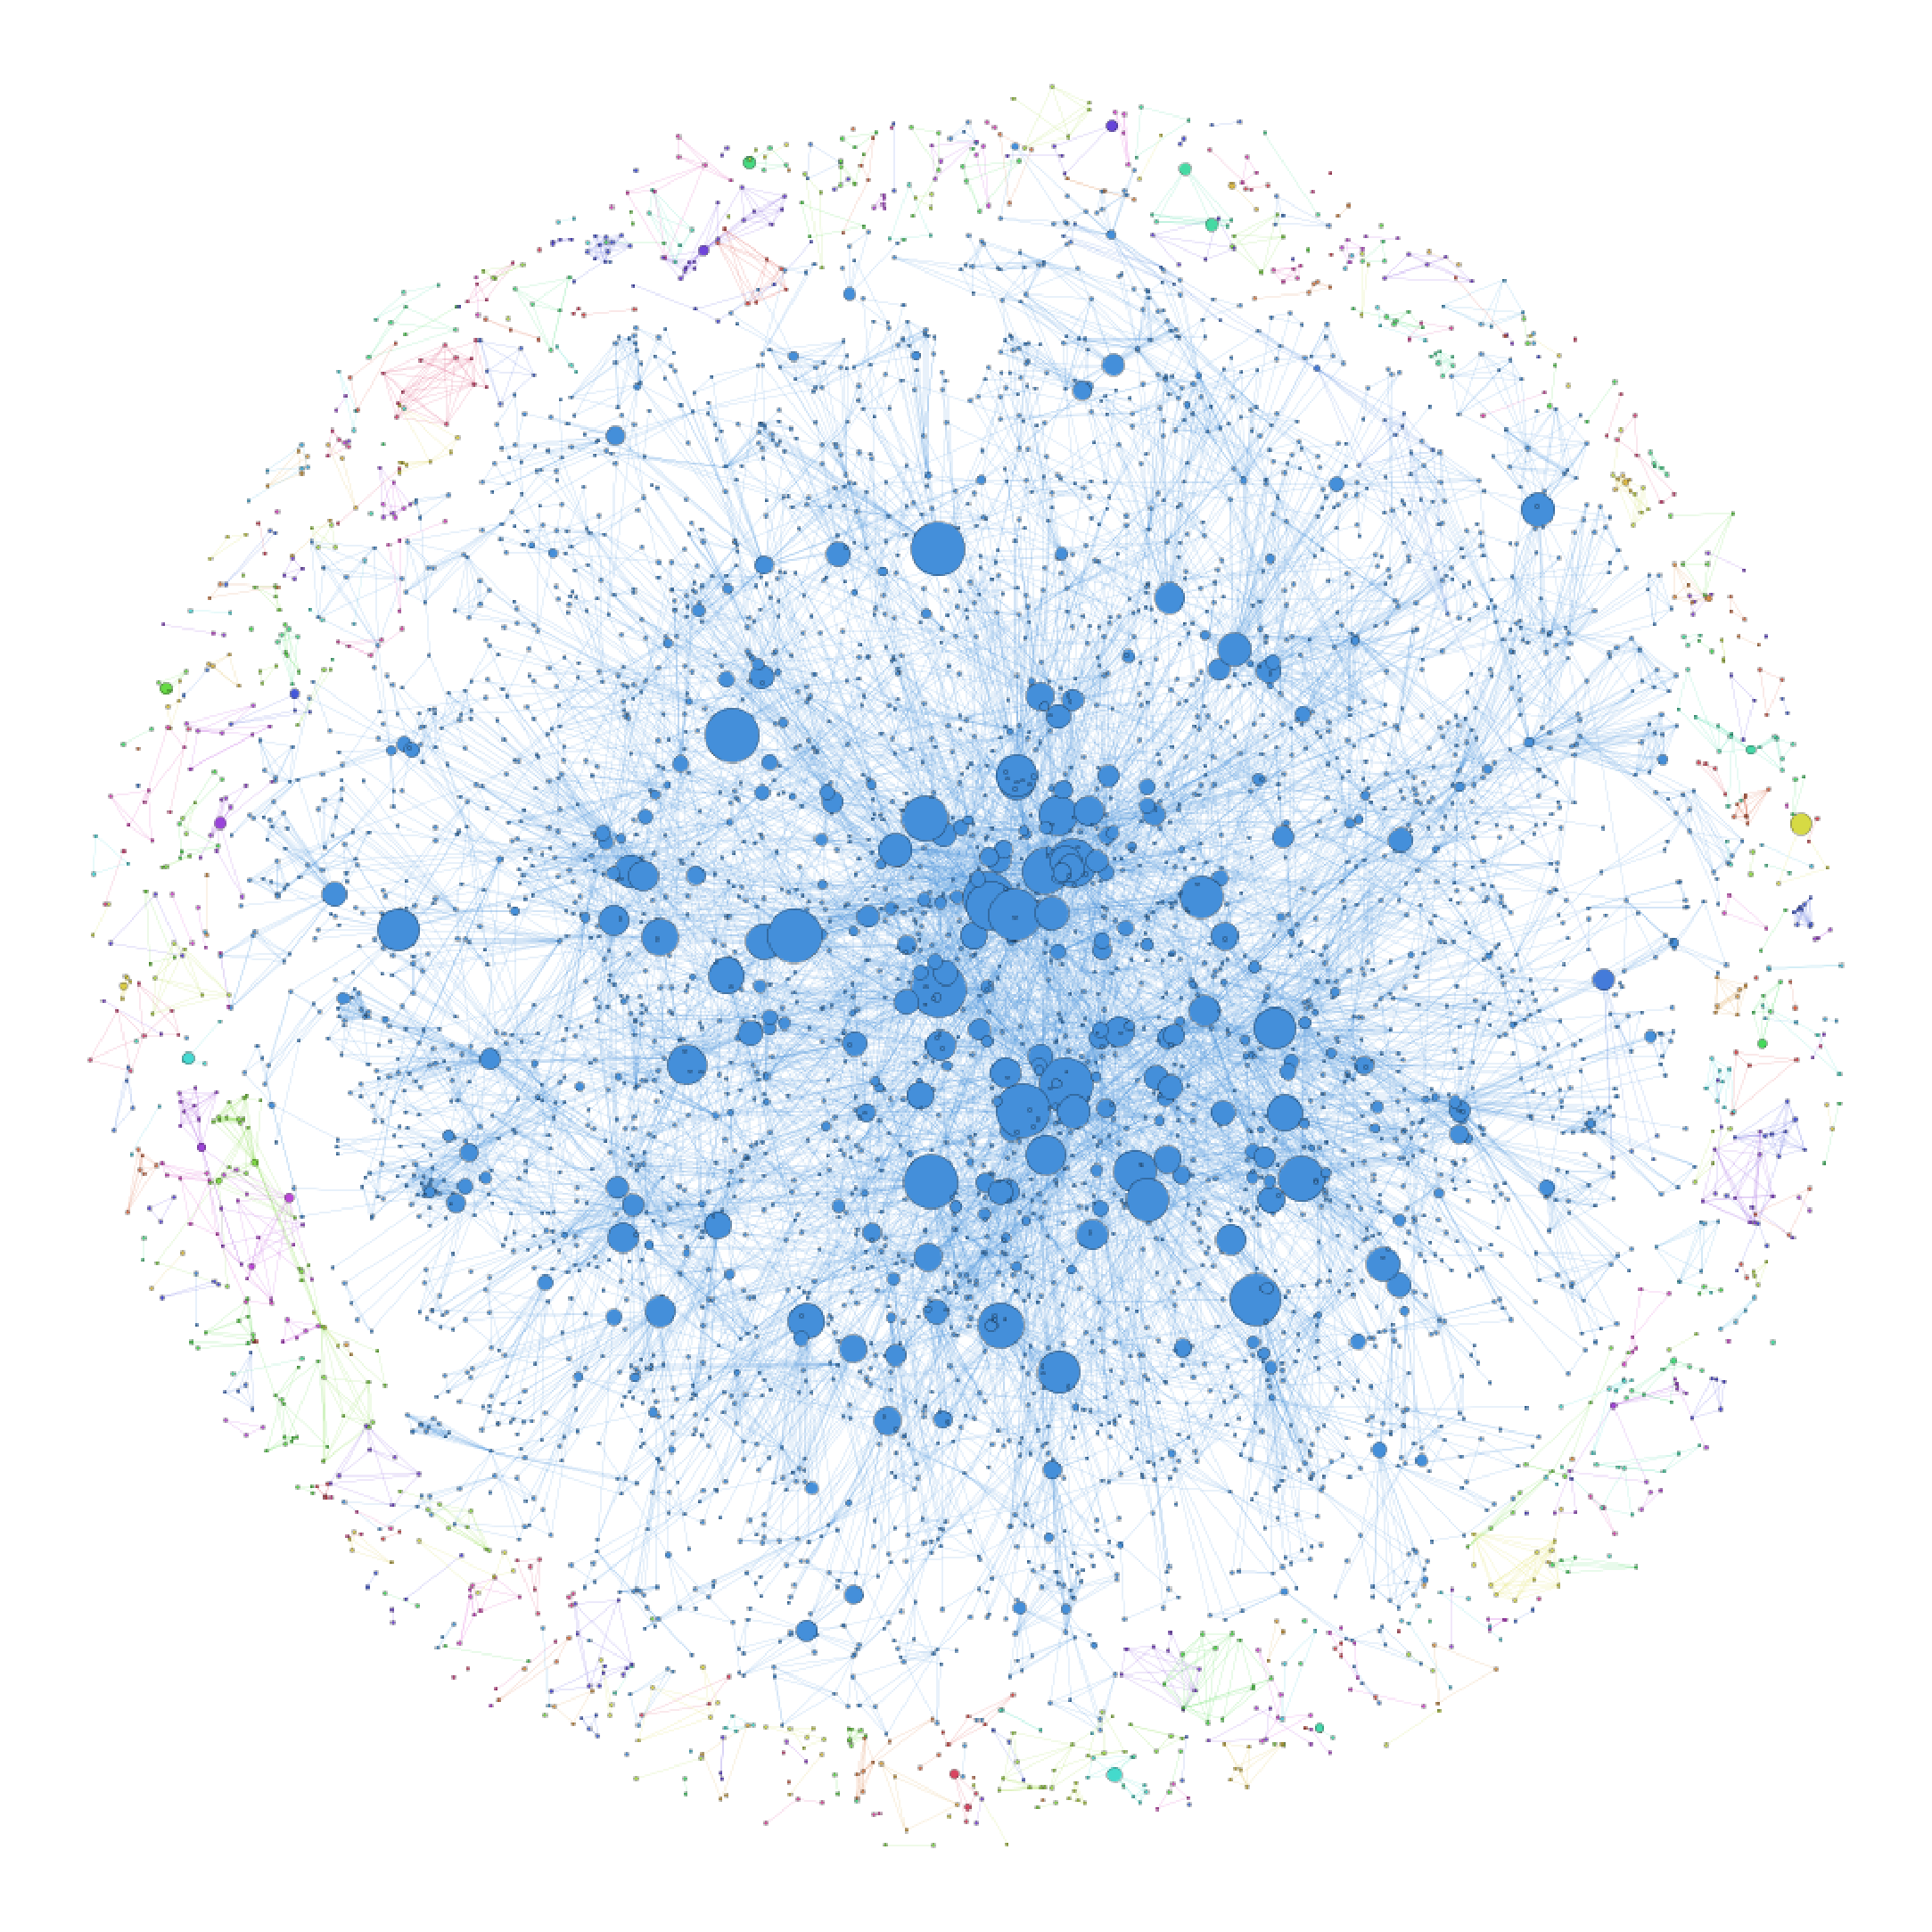
\includegraphics[scale=.21]{../graficos/network/chi.eps}
  }%
  \\
    \subfloat[SAC]{%
    \label{fig:rede_sac}
    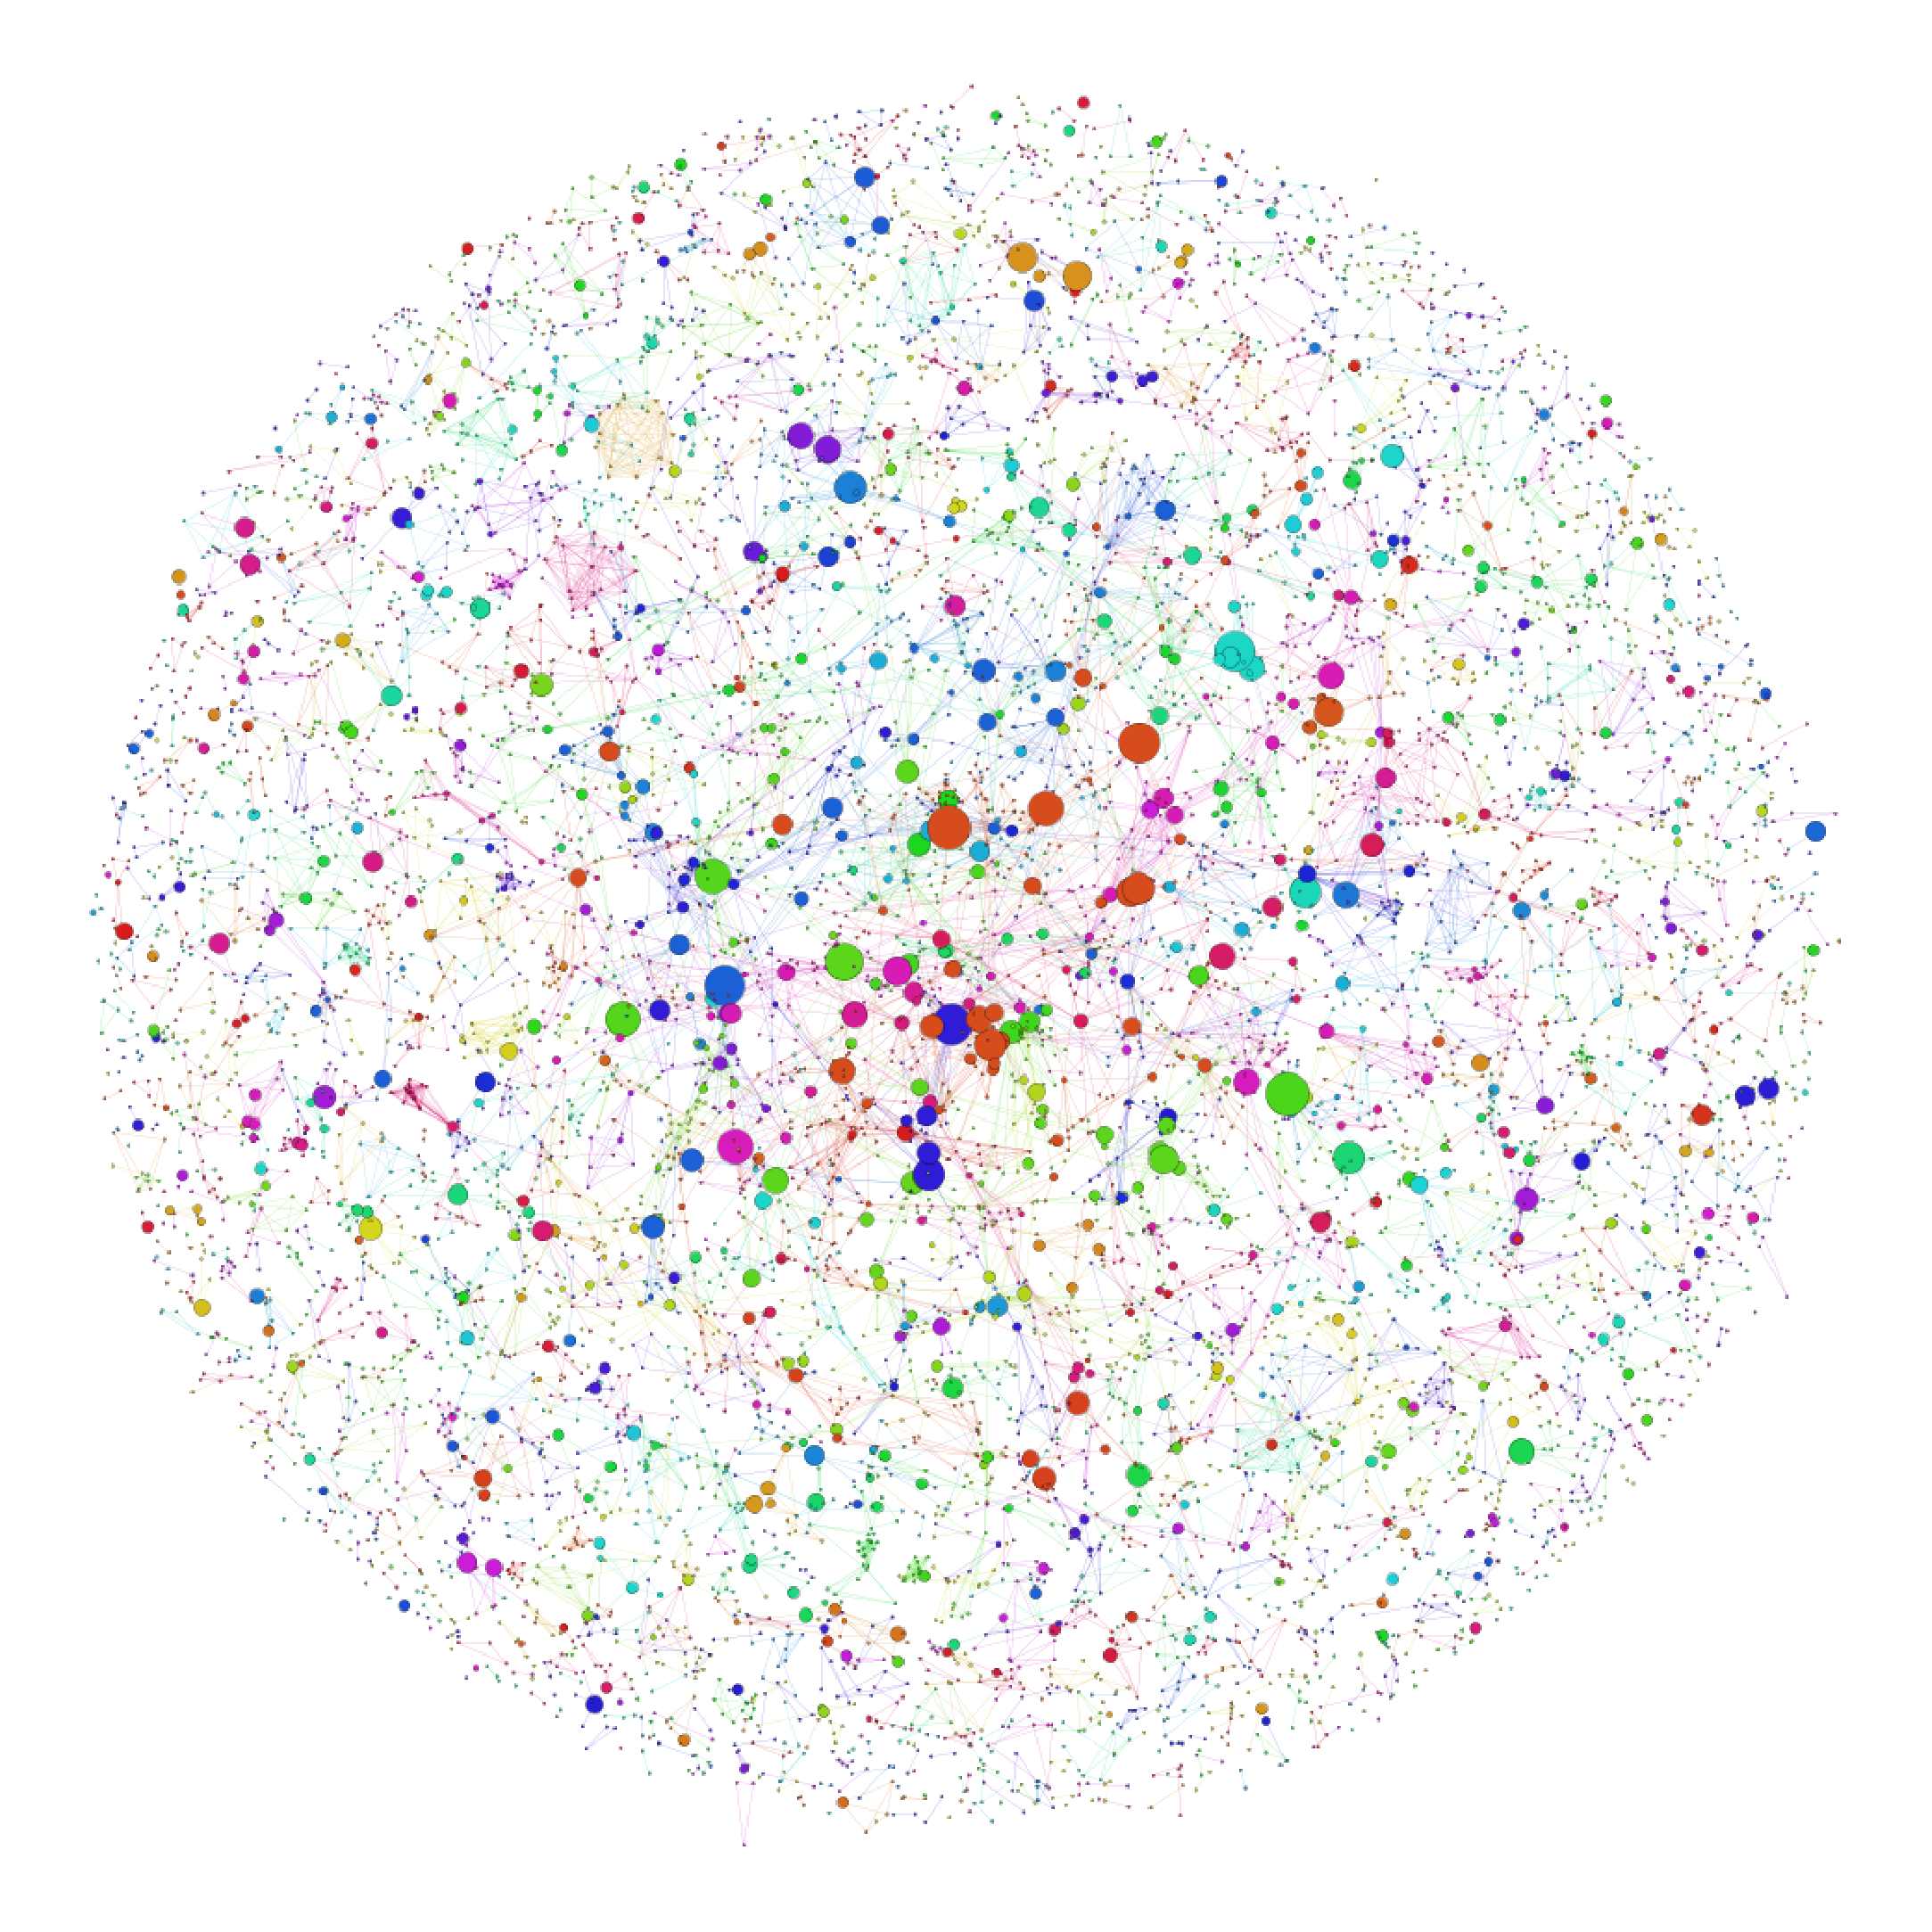
\includegraphics[scale=.21]{../graficos/network/sac.eps}
  }%
  \subfloat[STOC]{%
    \label{fig:rede_stoc}
    \includegraphics[scale=.21]{../graficos/network/stoc.eps}
  }%
  \end{center}
  \caption{Instância final das comunidades científicas}
  \label{fig:redes}
\end{figure}

\chapter{Conclusões e Trabalhos Futuros}\label{conclusao}

\section{Revisão do Trabalho}

Nesta dissertação apresentamos a caracterização de várias comunidades científicas presentes na DBLP, 
uma biblioteca digital da área de Ciência da Computação da qual extraímos e construímos 22 redes 
de colaboração científica. Em seguida, realizamos uma investigação profunda sobre os papéis que os membros 
dessas comunidades desempenham na formação e evolução topológica dessas redes.

Trabalhos anteriores estudam comunidades inteiras e são baseados em abordagens algorítmicas, 
tais como agrupamento hierárquico e \textit{k-means}, que buscam identificar grupos de nodos mais agrupados entre si 
do que ao restante da rede ou nodos que possuem alguma característica topológica. Diferentemente, focamos aqui em identificar os 
principais membros de uma comunidade que chamamos de núcleo da comunidade. Para determinar este núcleo, primeiramente 
definimos uma nova métrica chamada de \textit{CoScore}, derivada do índice~h. Como nossas análises são 
focadas na evolução temporal dessas comunidades, realizamos um estudo para estimar o índice~h de um dado pesquisador ao 
longo do tempo. Utilizamos dados coletados pelo projeto SHINE e comparamos várias estratégias de evolução para este 
índice, demonstrando que a estratégia final escolhida possui forte correlação positiva com os respectivos valores 
do Google Citations, uma ferramenta largamente utilizada pela comunidade 
científica para estimar o índice~h de um pesquisador. Assim, nossa métrica é capaz de capturar 
tanto a prolificidade de um pesquisador, quanto o seu envolvimento em uma comunidade ao longo do tempo. 

Após quantificar a importância de cada membro de uma comunidade, definimos dois importantes limiares 
para nosso estudo, o tamanho do núcleo da comunidade e o tamanho da janela temporal, sendo estes 
10\% e 3 anos, respectivamente. Nossos resultados indicam que membros dos núcleos são 
pesquisadores que contribuem ativamente com publicações para suas comunidades e possuem posição de 
destaque nelas. Desta forma, mostramos que vários desses membros foram premiados por suas contribuições 
à sua comunidade, incluindo até mesmo alguns que receberam o ACM \textit{A.M. Turing Award}.

Nossas análises mostraram, ainda, que o coeficiente de agrupamento dos membros do núcleo tende, de forma geral, a ser 
menor do que os dos demais membros da rede. No entanto, o valor da métrica \textit{betweenness} dos membros 
do núcleo tende a ser consideravelmente maior do que a dos não membros, indicando 
que membros dos núcleos atuam como pontes que interligam pequenos grupos de pesquisa. Além disso, 
observamos que os membros dos núcleos tendem a aumentar o grau médio, diâmetro, caminho mínimo médio e o 
tamanho do maior componente conectado da rede, e diminuir a assortatividade e o coeficiente de agrupamento.
Mais importante, observamos que as variações observadas nos conjuntos de membros dos núcleos das comunidades estão fortemente correlacionadas 
com as variações nas propriedades topológicas da rede. 

Finalmente, fornecemos uma representação visual dessas comunidades que reforça nossas análises e observações. 
Nossos resultados também destacam a importância de se estudar a relevância dos membros dos núcleos das comunidades e esperamos 
que nossas observações possam inspirar futuros modelos de formação de comunidade.


% Neste trabalho apresentamos uma investigação profunda dos papéis que os membros do núcleo das 
% comunidades científicas desempenham na formação e evolução da estrutura da rede de coautoria. Nosso esforço 
% se baseia em estudos anteriores existentes, uma vez que se concentra no núcleo de comunidades, em vez de 
% analisar os aspectos evolutivos de comunidades inteiras. Para isso, definimos um núcleo para as comunidades 
% baseado em uma nova métrica, ou seja, \textit{CoScore}, uma métrica derivada do índice~h que captura 
% tanto, a prolificidade, quanto o envolvimento de pesquisadores em uma comunidade. Nossas análises sugerem que membros 
% do núcleo da comunidade atuam como pontes que conectam pequenos grupos de pesquisa. Além disso, observamos que 
% os membros do núcleo das comunidades tendem a aumentar o grau médio da rede e diminuir a assortatividade. 
% Mais importante, observamos que as variações nos membros do núcleo da comunidade estão fortemente correlacionadas 
% com as variações nas propriedades de rede. Nosso estudo também destaca a importância de estudar os membros 
% do núcleo da comunidade e esperamos que nossas observações possam inspirar futuros modelos de formação da comunidade.

\section{Trabalhos Futuros}

A partir dos resultados do nosso estudo algumas oportunidades de trabalhos futuros foram identificadas e são listadas a seguir:

\begin{itemize}
  \item \textbf{Aplicação do estudo em outros contextos.} Nossas análises do núcleo das comunidades são aplicáveis a outros 
		contextos, como jogos multijogador massivo, OSNs e repositórios de outras 
		naturezas, como filmes e livros.
  \item \textbf{Utilização de outras métricas de prolificidade.} Existem outras métricas capazes de medir a 
		prolificidade de um pesquisador além do índice~h que poderiam também serem utilizadas no cálculo do 
		\textit{CoScore}, como o índice~g \citep{Egghe2006}.
  \item \textbf{Avaliação do \textit{CoScore} em outros contextos.} Nossa métrica quantifica a importância dos 
	        membros das comunidades. Desta forma, também poderíamos utilizá-la em outros contextos, e.g., para predição 
	        de \textit{links} e em sistemas de recomendação.
  \item \textbf{Geração de modelos de formação de comunidades.} O \textit{CoScore} pode ser combinado a outras
	        métricas para mapear o comportamento de como nodos e arestas surgem na rede, possibilitando a 
	        geração de modelos de formação de comunidades, conforme resultados prévios apresentados por \cite{Leskovec2005, Leskovec2008}.
  \item \textbf{Aplicação da abordagem proposta para o estudo de \textit{clusters}.} Vários trabalhos na literatura utilizam
	        abordagens algorítmicas para identificação de \textit{clusters} e de nodos importantes na topologia da rede. No entanto, 
	        essas abordagens possuem um custo computacional considerável. Assim sendo, seria interessante aplicar a nossa abordagem 
	        em estudos semelhantes.
  \item \textbf{Análise do impacto da migração de pesquisadores entre comunidades.} A migração dos membros do núcleo de uma comunidade
		pode ser utilizada para prever o sucesso ou declínio dessa comunidade. Sendo assim, nossa métrica poderia ser aplicada
		em estudos que visem caracterizar a migração de membros de um comunidade ou até inspirar modelos capazes de predizer tais migrações.
\end{itemize}


% Como trabalho futuro, gostaríamos de estender e aplicar nossa análise do núcleo da comunidade para 
% outros contextos, como jogos multijogador massivo, redes sociais online e repositórios de outras naturezas, como filmes e livros.

% In this work we provide a deep investigation of the roles that members of the core of scientific communities play in the coauthorship network structure formation and evolution.
% Our effort builds upon previous existent studies as it focuses on the core community instead of analyzing the evolutionary aspects of entire communities.  To do that, we defined a
% community core based on a new metric, namely \etxtit{core score}, an h-index derived metric that captures both, the prolificness and the involvement of researchers in a community. Our analysis
% suggests that the members of the core community work as bridges that connect smaller clustered research groups. Additionally, we noted that the members of the core community tend to
% increase the average degree of the network and decrease the assortativeness. More important, we noted that variations on the members of the community core are strongly correlated
% with variations on network properties.  Our study also highlights the importance to study the members of the community core and we hope that our observations might inspire future
% community formation models.
% 
% As future work, we would like to extend and apply our analysis of the community core to other contexts such as massive multiplayer games and on-line social networks.
% Aqui vem a parte da bibliografia: use o comando \ufmgbibliography indicando
% apenas o nome do arquivo .bib (sem a extensão).
\ppgccbibliography{referencias} % ARQUIVO CONTENDO A BIBLIOGRAFIA
% \bibliography{referencias}
\begin{appendices}

%%%%%%%%%%%%%%%%%%%%%%%%%%%%%%%%%%%
\chapter{Média dos Valores de \textit{Resemblance}}\label{apendice:media_valores_resemblance}
%%%%%%%%%%%%%%%%%%%%%%%%%%%%%%%%%%%

\begin{figure}[!htb]
  \begin{center}
    \subfloat[CCS]{%
      \label{fig:ccs_slide_window_top_list}
      \includegraphics[scale=.6]{../graficos/window_core_size/pt_BR/ccs_arithmetic_slide_window_arithmetic_top_list.eps}
    }%
    \subfloat[CIKM]{%
      \label{fig:cikm_slide_window_top_list}
      \includegraphics[scale=.6]{../graficos/window_core_size/pt_BR/cikm_arithmetic_slide_window_arithmetic_top_list.eps}
    }%
    \\
    \subfloat[DAC]{%
      \label{fig:dac_slide_window_top_list}
      \includegraphics[scale=.6]{../graficos/window_core_size/pt_BR/dac_arithmetic_slide_window_arithmetic_top_list.eps}
    }%
    \subfloat[HSCC]{%
      \label{fig:hscc_slide_window_top_list}
      \includegraphics[scale=.6]{../graficos/window_core_size/pt_BR/hscc_arithmetic_slide_window_arithmetic_top_list.eps}
    }%
    \phantomcaption
  \end{center}
\end{figure}
\begin{figure}[!htb]
  \begin{center}
    \ContinuedFloat
    \subfloat[ICSE]{%
      \label{fig:icse_slide_window_top_list}
      \includegraphics[scale=.6]{../graficos/window_core_size/pt_BR/icse_arithmetic_slide_window_arithmetic_top_list.eps}
    }%
    \subfloat[ISCA]{%
      \label{fig:isca_slide_window_top_list}
      \includegraphics[scale=.6]{../graficos/window_core_size/pt_BR/isca_arithmetic_slide_window_arithmetic_top_list.eps}
    }%
    \\
    \subfloat[KDD]{%
      \label{fig:kdd_slide_window_top_list}
      \includegraphics[scale=.6]{../graficos/window_core_size/pt_BR/kdd_arithmetic_slide_window_arithmetic_top_list.eps}
    }%
    \subfloat[MICRO]{%
      \label{fig:micro_slide_window_top_list}
      \includegraphics[scale=.6]{../graficos/window_core_size/pt_BR/micro_arithmetic_slide_window_arithmetic_top_list.eps}
    }%
    \\
    \subfloat[MM]{%
      \label{fig:mm_slide_window_top_list}
      \includegraphics[scale=.6]{../graficos/window_core_size/pt_BR/acm_multimedia_arithmetic_slide_window_arithmetic_top_list.eps}
    }%
    \subfloat[MOBICOM]{%
      \label{fig:mobicom_slide_window_top_list}
      \includegraphics[scale=.6]{../graficos/window_core_size/pt_BR/mobicom_arithmetic_slide_window_arithmetic_top_list.eps}
    }%
  \end{center}
\end{figure}    
\begin{figure}[!htb]
  \begin{center}
    \ContinuedFloat
    \subfloat[PODC]{%
      \label{fig:podc_slide_window_top_list}
      \includegraphics[scale=.6]{../graficos/window_core_size/pt_BR/podc_arithmetic_slide_window_arithmetic_top_list.eps}
    }% 
    \subfloat[POPL]{%
      \label{fig:popl_slide_window_top_list}
      \includegraphics[scale=.6]{../graficos/window_core_size/pt_BR/popl_arithmetic_slide_window_arithmetic_top_list.eps}
    }%
    \\
    \subfloat[SAC]{%
      \label{fig:sac_slide_window_top_list}
      \includegraphics[scale=.6]{../graficos/window_core_size/pt_BR/sac_arithmetic_slide_window_arithmetic_top_list.eps}
    }%
    \subfloat[SIGCOMM]{%
      \label{fig:sigcomm_slide_window_top_list}
      \includegraphics[scale=.6]{../graficos/window_core_size/pt_BR/sigcomm_arithmetic_slide_window_arithmetic_top_list.eps}
    }%
    \\
    \subfloat[SIGCSE]{%
      \label{fig:sigcse_slide_window_top_list}
      \includegraphics[scale=.6]{../graficos/window_core_size/pt_BR/sigcse_arithmetic_slide_window_arithmetic_top_list.eps}
    }%
    \subfloat[SIGDOC]{%
      \label{fig:sigdoc_slide_window_top_list}
      \includegraphics[scale=.6]{../graficos/window_core_size/pt_BR/sigdoc_arithmetic_slide_window_arithmetic_top_list.eps}
    }%
  \end{center}
\end{figure}    
\begin{figure}[!htb]
  \begin{center}
    \ContinuedFloat
    \subfloat[SIGGRAPH]{%
      \label{fig:siggraph_slide_window_top_list}
      \includegraphics[scale=.6]{../graficos/window_core_size/pt_BR/siggraph_arithmetic_slide_window_arithmetic_top_list.eps}
    }%
    \subfloat[SIGIR]{%
      \label{fig:sigir_slide_window_top_list}
      \includegraphics[scale=.6]{../graficos/window_core_size/pt_BR/sigir_arithmetic_slide_window_arithmetic_top_list.eps}
    }%
    \\
    \subfloat[SIGMETRICS]{%
      \label{fig:sigmetrics_slide_window_top_list}
      \includegraphics[scale=.6]{../graficos/window_core_size/pt_BR/sigmetrics_arithmetic_slide_window_arithmetic_top_list.eps}
    }%
    \subfloat[STOC]{%
      \label{fig:stoc_slide_window_top_list}
      \includegraphics[scale=.6]{../graficos/window_core_size/pt_BR/stoc_arithmetic_slide_window_arithmetic_top_list.eps}
    }%
  \end{center}
\caption{Média dos valores de \textit{resemblance}}
\label{fig:averange_values_resemblance_appendice}
\end{figure}

%%%%%%%%%%%%%%%%%%%%%%%%%%%%%%%%%%%
\chapter{Métricas de Evolução das Comunidades Científicas}\label{apendice:metricas_evolucao_comunidades}
%%%%%%%%%%%%%%%%%%%%%%%%%%%%%%%%%%%

Neste apêndice apresentamos as métricas das demais conferências, separada entre três grupos. O grupo A é constituído pelas conferências
CIKM, CHI, KDD, SAC e SIGCOMM, o grupo B pelas conferências CSS, MICRO, MM, MOBICOM e SIGDOC, e o grupo C pelas conferências
HSCC, ICSE, ISCA, SIGCSE, SIGGRAPH e SIGMETRICS.

\begin{figure}[!htb]
  \begin{center}
  \subfloat[Assortatividade final - Grupo A]{%
    \label{fig:assortativity_1_in_1_apendice_grupa_a}
    \includegraphics[scale=.6]{../graficos/sigs_metricas_acumuladas_1_em_1_ano/pt_BR/assortatividade_grupo_temporal_web_apendice_1.eps}
  }%
  \subfloat[Assortatividade por janela - Grupo A]{%
    \label{fig:assortativity_slide_window_apendice_grupa_a}
    \includegraphics[scale=.6]{../graficos/core_over_time/metricas_tradicionais/pt_BR/assortatividade_slide_window_grupo_temporal_web_apendice_1.eps}
  }%
  \phantomcaption
  \end{center}
\end{figure}
\begin{figure}[!htb]
  \begin{center}
  \ContinuedFloat
  \subfloat[Assortatividade final - Grupo B]{%
    \label{fig:assortativity_1_in_1_apendice_grupa_b}
    \includegraphics[scale=.6]{../graficos/sigs_metricas_acumuladas_1_em_1_ano/pt_BR/assortatividade_grupo_temporal_web_apendice_2.eps}
  }%
  \subfloat[Assortatividade por janela - Grupo B]{%
    \label{fig:assortativity_slide_window_apendice_grupa_b}
    \includegraphics[scale=.6]{../graficos/core_over_time/metricas_tradicionais/pt_BR/assortatividade_slide_window_grupo_temporal_web_apendice_2.eps}
  }%
  \\
  \subfloat[Assortatividade final - Grupo C]{%
    \label{fig:assortativity_1_in_1_apendice_grupa_c}
    \includegraphics[scale=.6]{../graficos/sigs_metricas_acumuladas_1_em_1_ano/pt_BR/assortatividade_grupo_temporal_web_apendice_3.eps}
  }%
  \subfloat[Assortatividade por janela - Grupo C]{%
    \label{fig:assortativity_slide_window_apendice_grupa_c}
    \includegraphics[scale=.6]{../graficos/core_over_time/metricas_tradicionais/pt_BR/assortatividade_slide_window_grupo_temporal_web_apendice_3.eps}
  }%
  \end{center}
  \caption{Assortatividade das comunidades científicas}
  \label{fig:metrics_assortativity_apendice}
\end{figure}


\begin{figure}[!htb]
  \begin{center}
  \subfloat[CMM final - Grupo A]{%
    \label{fig:average_shortest_1_in_1_apendice_grupa_a}
    \includegraphics[scale=.6]{../graficos/sigs_metricas_acumuladas_1_em_1_ano/pt_BR/caminho_minimo_medio_grupo_temporal_web_apendice_1.eps}
  }%
  \subfloat[CMM por janela - Grupo A]{%
    \label{fig:average_shortest_slide_window_apendice_grupa_a}
    \includegraphics[scale=.6]{../graficos/core_over_time/metricas_tradicionais/pt_BR/caminho_minimo_medio_slide_window_grupo_temporal_web_apendice_1.eps}
  }%
  \phantomcaption
  \end{center}
\end{figure}
\begin{figure}[!htb]
  \begin{center}
  \ContinuedFloat
  \subfloat[CMM final - Grupo B]{%
    \label{fig:average_shortest_1_in_1_apendice_grupa_b}
    \includegraphics[scale=.6]{../graficos/sigs_metricas_acumuladas_1_em_1_ano/pt_BR/caminho_minimo_medio_grupo_temporal_web_apendice_2.eps}
  }%
  \subfloat[CMM por janela - Grupo B]{%
    \label{fig:average_shortest_slide_window_apendice_grupa_b}
    \includegraphics[scale=.6]{../graficos/core_over_time/metricas_tradicionais/pt_BR/caminho_minimo_medio_slide_window_grupo_temporal_web_apendice_2.eps}
  }%
  \\
  \subfloat[CMM final - Grupo C]{%
    \label{fig:average_shortest_1_in_1_apendice_grupa_c}
    \includegraphics[scale=.6]{../graficos/sigs_metricas_acumuladas_1_em_1_ano/pt_BR/caminho_minimo_medio_grupo_temporal_web_apendice_3.eps}
  }%
  \subfloat[CMM por janela - Grupo C]{%
    \label{fig:average_shortest_slide_window_apendice_grupa_c}
    \includegraphics[scale=.6]{../graficos/core_over_time/metricas_tradicionais/pt_BR/caminho_minimo_medio_slide_window_grupo_temporal_web_apendice_3.eps}
  }%
  \end{center}
  \caption{Caminho mínimo médio das comunidades científicas}
  \label{fig:metrics_average_shortest_apendice}
\end{figure}


\begin{figure}[!htb]
  \begin{center}
  \subfloat[CA final - Grupo A]{%
    \label{fig:average_shortest_1_in_1_apendice_grupa_a}
    \includegraphics[scale=.6]{../graficos/sigs_metricas_acumuladas_1_em_1_ano/pt_BR/coeficiente_agrupamento_grupo_temporal_web_apendice_1.eps}
  }%
  \subfloat[CA por janela - Grupo A]{%
    \label{fig:average_shortest_slide_window_apendice_grupa_a}
    \includegraphics[scale=.6]{../graficos/core_over_time/metricas_tradicionais/pt_BR/coeficiente_agrupamento_slide_window_grupo_temporal_web_apendice_1.eps}
  }%
  \phantomcaption
  \end{center}
\end{figure}
\begin{figure}[!htb]
  \begin{center}
  \ContinuedFloat
  \subfloat[CA final - Grupo B]{%
    \label{fig:average_shortest_1_in_1_apendice_grupa_b}
    \includegraphics[scale=.6]{../graficos/sigs_metricas_acumuladas_1_em_1_ano/pt_BR/coeficiente_agrupamento_grupo_temporal_web_apendice_2.eps}
  }%
  \subfloat[CA por janela - Grupo B]{%
    \label{fig:average_shortest_slide_window_apendice_grupa_b}
    \includegraphics[scale=.6]{../graficos/core_over_time/metricas_tradicionais/pt_BR/coeficiente_agrupamento_slide_window_grupo_temporal_web_apendice_2.eps}
  }%
  \\
  \subfloat[CA final - Grupo C]{%
    \label{fig:average_shortest_1_in_1_apendice_grupa_c}
    \includegraphics[scale=.6]{../graficos/sigs_metricas_acumuladas_1_em_1_ano/pt_BR/coeficiente_agrupamento_grupo_temporal_web_apendice_3.eps}
  }%
  \subfloat[CA por janela - Grupo C]{%
    \label{fig:average_shortest_slide_window_apendice_grupa_c}
    \includegraphics[scale=.6]{../graficos/core_over_time/metricas_tradicionais/pt_BR/coeficiente_agrupamento_slide_window_grupo_temporal_web_apendice_3.eps}
  }%
  \end{center}
  \caption{Coeficiente de agrupamento das comunidades científicas}
  \label{fig:metrics_average_shortest_apendice}
\end{figure}


\begin{figure}[!htb]
  \begin{center}
  \subfloat[Maior CFC final - Grupo A]{%
    \label{fig:average_shortest_1_in_1_apendice_grupa_a}
    \includegraphics[scale=.6]{../graficos/sigs_metricas_acumuladas_1_em_1_ano/pt_BR/porcentagem_maior_componente_grupo_temporal_web_apendice_1.eps}
  }%
  \subfloat[Maior CFC por janela - Grupo A]{%
    \label{fig:average_shortest_slide_window_apendice_grupa_a}
    \includegraphics[scale=.6]{../graficos/core_over_time/metricas_tradicionais/pt_BR/porcentagem_maior_componente_slide_window_grupo_temporal_web_apendice_1.eps}
  }%
  \phantomcaption
  \end{center}
\end{figure}
\begin{figure}[!htb]
  \begin{center}
  \ContinuedFloat
  \subfloat[Maior CFC final - Grupo B]{%
    \label{fig:average_shortest_1_in_1_apendice_grupa_b}
    \includegraphics[scale=.6]{../graficos/sigs_metricas_acumuladas_1_em_1_ano/pt_BR/porcentagem_maior_componente_grupo_temporal_web_apendice_2.eps}
  }%
  \subfloat[Maior CFC por janela - Grupo B]{%
    \label{fig:average_shortest_slide_window_apendice_grupa_b}
    \includegraphics[scale=.6]{../graficos/core_over_time/metricas_tradicionais/pt_BR/porcentagem_maior_componente_slide_window_grupo_temporal_web_apendice_2.eps}
  }%
  \\
  \subfloat[Maior CFC final - Grupo C]{%
    \label{fig:average_shortest_1_in_1_apendice_grupa_c}
    \includegraphics[scale=.6]{../graficos/sigs_metricas_acumuladas_1_em_1_ano/pt_BR/porcentagem_maior_componente_grupo_temporal_web_apendice_3.eps}
  }%
  \subfloat[Maior CFC por janela - Grupo C]{%
    \label{fig:average_shortest_slide_window_apendice_grupa_c}
    \includegraphics[scale=.6]{../graficos/core_over_time/metricas_tradicionais/pt_BR/porcentagem_maior_componente_slide_window_grupo_temporal_web_apendice_3.eps}
  }%
  \end{center}
  \caption{Maior CFC das comunidades científicas}
  \label{fig:metrics_average_shortest_apendice}
\end{figure}


\begin{figure}[!htb]
  \begin{center}
  \subfloat[Grau médio final - Grupo A]{%
    \label{fig:average_shortest_1_in_1_apendice_grupa_a}
    \includegraphics[scale=.6]{../graficos/sigs_metricas_acumuladas_1_em_1_ano/pt_BR/grau_medio_nodos_grupo_temporal_web_apendice_1.eps}
  }%
  \subfloat[Grau médio por janela - Grupo A]{%
    \label{fig:average_shortest_slide_window_apendice_grupa_a}
    \includegraphics[scale=.6]{../graficos/core_over_time/metricas_tradicionais/pt_BR/grau_medio_nodos_slide_window_grupo_temporal_web_apendice_1.eps}
  }%
  \phantomcaption
  \end{center}
\end{figure}
\begin{figure}[!htb]
  \begin{center}
  \ContinuedFloat
  \subfloat[Grau médio final - Grupo B]{%
    \label{fig:average_shortest_1_in_1_apendice_grupa_b}
    \includegraphics[scale=.6]{../graficos/sigs_metricas_acumuladas_1_em_1_ano/pt_BR/grau_medio_nodos_grupo_temporal_web_apendice_2.eps}
  }%
  \subfloat[Grau médio por janela - Grupo B]{%
    \label{fig:average_shortest_slide_window_apendice_grupa_b}
    \includegraphics[scale=.6]{../graficos/core_over_time/metricas_tradicionais/pt_BR/grau_medio_nodos_slide_window_grupo_temporal_web_apendice_2.eps}
  }%
  \\
  \subfloat[Grau médio final - Grupo C]{%
    \label{fig:average_shortest_1_in_1_apendice_grupa_c}
    \includegraphics[scale=.6]{../graficos/sigs_metricas_acumuladas_1_em_1_ano/pt_BR/grau_medio_nodos_grupo_temporal_web_apendice_3.eps}
  }%
  \subfloat[Grau médio por janela - Grupo C]{%
    \label{fig:average_shortest_slide_window_apendice_grupa_c}
    \includegraphics[scale=.6]{../graficos/core_over_time/metricas_tradicionais/pt_BR/grau_medio_nodos_slide_window_grupo_temporal_web_apendice_3.eps}
  }%
  \end{center}
  \caption{Grau médio das comunidades científicas}
  \label{fig:metrics_average_shortest_apendice}
\end{figure}

%%%%%%%%%%%%%%%%%%%%%%%%%%%%%%%%%%%
\chapter{Comparação entre Membros e Não Membros}\label{apendice:comparacao_nucleo}
%%%%%%%%%%%%%%%%%%%%%%%%%%%%%%%%%%%

\begin{figure}[!htb]
  \begin{center}
  \subfloat[Coeficiente de agrupamento]{%
    \label{fig:core_com_ccs_clustering_coefficient_apendice}
    \includegraphics[scale=.6]{../graficos/core_over_time/core_community/pt_BR/ccs_janela_3_core_coeficiente_agrupamento.eps}
  }
  \subfloat[Grau médio]{%
    \label{fig:core_com_ccs_average_degree_apendice}
    \includegraphics[scale=.6]{../graficos/core_over_time/core_community/pt_BR/ccs_janela_3_core_grau_medio_nodos.eps}
  }
  \phantomcaption
  \end{center}
\end{figure}
\begin{figure}[!htb]
  \begin{center}
  \ContinuedFloat
  \subfloat[Maior CFC]{%
    \label{fig:core_com_ccs_largest_connected_component_apendice}
    \includegraphics[scale=.6]{../graficos/core_over_time/core_community/pt_BR/ccs_janela_3_core_maior_componente_conectado.eps}
  }
  \subfloat[\textit{Betweenness} médio]{%
    \label{fig:core_com_ccs_betweenness_apendice}
    \includegraphics[scale=.6]{../graficos/core_over_time/core_community/pt_BR/ccs_janela_3_core_betweenness.eps}
  }
  \end{center}
  \caption{Propriedades da comunidade CCS para os membros e não membros do núcleo}
  \label{fig:metrics_comparing_core_community_ccs_apendice}
\end{figure}

\begin{figure}[!htb]
  \begin{center}
  \subfloat[Coeficiente de agrupamento]{%
    \label{fig:core_com_chi_clustering_coefficient_apendice}
    \includegraphics[scale=.6]{../graficos/core_over_time/core_community/pt_BR/chi_janela_3_core_coeficiente_agrupamento.eps}
  }
  \subfloat[Grau médio]{%
    \label{fig:core_com_chi_average_degree_apendice}
    \includegraphics[scale=.6]{../graficos/core_over_time/core_community/pt_BR/chi_janela_3_core_grau_medio_nodos.eps}
  }
  \\
  \subfloat[Maior CFC]{%
    \label{fig:core_com_chi_largest_connected_component_apendice}
    \includegraphics[scale=.6]{../graficos/core_over_time/core_community/pt_BR/chi_janela_3_core_maior_componente_conectado.eps}
  }
  \subfloat[\textit{Betweenness} médio]{%
    \label{fig:core_com_chi_betweenness_apendice}
    \includegraphics[scale=.6]{../graficos/core_over_time/core_community/pt_BR/chi_janela_3_core_betweenness.eps}
  }
  \end{center}
  \caption{Propriedades da comunidade CHI para os membros e não membros do núcleo}
  \label{fig:metrics_comparing_core_community_chi_apendice}
\end{figure}

\begin{figure}[!htb]
  \begin{center}
  \subfloat[Coeficiente de agrupamento]{%
    \label{fig:core_com_cikm_clustering_coefficient_apendice}
    \includegraphics[scale=.6]{../graficos/core_over_time/core_community/pt_BR/cikm_janela_3_core_coeficiente_agrupamento.eps}
  }
  \subfloat[Grau médio]{%
    \label{fig:core_com_cikm_average_degree_apendice}
    \includegraphics[scale=.6]{../graficos/core_over_time/core_community/pt_BR/cikm_janela_3_core_grau_medio_nodos.eps}
  }
  \\
  \subfloat[Maior CFC]{%
    \label{fig:core_com_cikm_largest_connected_component_apendice}
    \includegraphics[scale=.6]{../graficos/core_over_time/core_community/pt_BR/cikm_janela_3_core_maior_componente_conectado.eps}
  }
  \subfloat[\textit{Betweenness} médio]{%
    \label{fig:core_com_cikm_betweenness_apendice}
    \includegraphics[scale=.6]{../graficos/core_over_time/core_community/pt_BR/cikm_janela_3_core_betweenness.eps}
  }
  \end{center}
  \caption{Propriedades da comunidade CIKM para os membros e não membros do núcleo}
  \label{fig:metrics_comparing_core_community_cikm_apendice}
\end{figure}

\begin{figure}[!htb]
  \begin{center}
  \subfloat[Coeficiente de agrupamento]{%
    \label{fig:core_com_dac_clustering_coefficient_apendice}
    \includegraphics[scale=.6]{../graficos/core_over_time/core_community/pt_BR/dac_janela_3_core_coeficiente_agrupamento.eps}
  }
  \subfloat[Grau médio]{%
    \label{fig:core_com_dac_average_degree_apendice}
    \includegraphics[scale=.6]{../graficos/core_over_time/core_community/pt_BR/dac_janela_3_core_grau_medio_nodos.eps}
  }
\phantomcaption
  \end{center}
\end{figure}
\begin{figure}[!htb]
  \begin{center}
  \ContinuedFloat
  \subfloat[Maior CFC]{%
    \label{fig:core_com_dac_largest_connected_component_apendice}
    \includegraphics[scale=.6]{../graficos/core_over_time/core_community/pt_BR/dac_janela_3_core_maior_componente_conectado.eps}
  }
  \subfloat[\textit{Betweenness} médio]{%
    \label{fig:core_com_dac_betweenness_apendice}
    \includegraphics[scale=.6]{../graficos/core_over_time/core_community/pt_BR/dac_janela_3_core_betweenness.eps}
  }
  \end{center}
  \caption{Propriedades da comunidade DAC para os membros e não membros do núcleo}
  \label{fig:metrics_comparing_core_community_dac_apendice}
\end{figure}

\begin{figure}[!htb]
  \begin{center}
  \subfloat[Coeficiente de agrupamento]{%
    \label{fig:core_com_hscc_clustering_coefficient_apendice}
    \includegraphics[scale=.6]{../graficos/core_over_time/core_community/pt_BR/hscc_janela_3_core_coeficiente_agrupamento.eps}
  }
  \subfloat[Grau médio]{%
    \label{fig:core_com_hscc_average_degree_apendice}
    \includegraphics[scale=.6]{../graficos/core_over_time/core_community/pt_BR/hscc_janela_3_core_grau_medio_nodos.eps}
  }
  \\
  \subfloat[Maior CFC]{%
    \label{fig:core_com_hscc_largest_connected_component_apendice}
    \includegraphics[scale=.6]{../graficos/core_over_time/core_community/pt_BR/hscc_janela_3_core_maior_componente_conectado.eps}
  }
  \subfloat[\textit{Betweenness} médio]{%
    \label{fig:core_com_hscc_betweenness_apendice}
    \includegraphics[scale=.6]{../graficos/core_over_time/core_community/pt_BR/hscc_janela_3_core_betweenness.eps}
  }
  \end{center}
  \caption{Propriedades da comunidade HSCC para os membros e não membros do núcleo}
  \label{fig:metrics_comparing_core_community_hscc_apendice}
\end{figure}

\begin{figure}[!htb]
  \begin{center}
  \subfloat[Coeficiente de agrupamento]{%
    \label{fig:core_com_icse_clustering_coefficient_apendice}
    \includegraphics[scale=.6]{../graficos/core_over_time/core_community/pt_BR/icse_janela_3_core_coeficiente_agrupamento.eps}
  }
  \subfloat[Grau médio]{%
    \label{fig:core_com_icse_average_degree_apendice}
    \includegraphics[scale=.6]{../graficos/core_over_time/core_community/pt_BR/icse_janela_3_core_grau_medio_nodos.eps}
  }
  \\
  \subfloat[Maior CFC]{%
    \label{fig:core_com_icse_largest_connected_component_apendice}
    \includegraphics[scale=.6]{../graficos/core_over_time/core_community/pt_BR/icse_janela_3_core_maior_componente_conectado.eps}
  }
  \subfloat[\textit{Betweenness} médio]{%
    \label{fig:core_com_icse_betweenness_apendice}
    \includegraphics[scale=.6]{../graficos/core_over_time/core_community/pt_BR/icse_janela_3_core_betweenness.eps}
  }
  \end{center}
  \caption{Propriedades da comunidade ICSE para os membros e não membros do núcleo}
  \label{fig:metrics_comparing_core_community_icse_apendice}
\end{figure}

\begin{figure}[!htb]
  \begin{center}
  \subfloat[Coeficiente de agrupamento]{%
    \label{fig:core_com_isca_clustering_coefficient_apendice}
    \includegraphics[scale=.6]{../graficos/core_over_time/core_community/pt_BR/isca_janela_3_core_coeficiente_agrupamento.eps}
  }
  \subfloat[Grau médio]{%
    \label{fig:core_com_isca_average_degree_apendice}
    \includegraphics[scale=.6]{../graficos/core_over_time/core_community/pt_BR/isca_janela_3_core_grau_medio_nodos.eps}
  }
  \phantomcaption
  \end{center}
\end{figure}
\begin{figure}[!htb]
  \begin{center}
  \ContinuedFloat
  \subfloat[Maior CFC]{%
    \label{fig:core_com_isca_largest_connected_component_apendice}
    \includegraphics[scale=.6]{../graficos/core_over_time/core_community/pt_BR/isca_janela_3_core_maior_componente_conectado.eps}
  }
  \subfloat[\textit{Betweenness} médio]{%
    \label{fig:core_com_isca_betweenness_apendice}
    \includegraphics[scale=.6]{../graficos/core_over_time/core_community/pt_BR/isca_janela_3_core_betweenness.eps}
  }
  \end{center}
  \caption{Propriedades da comunidade ISCA para os membros e não membros do núcleo}
  \label{fig:metrics_comparing_core_community_isca_apendice}
\end{figure}

\begin{figure}[!htb]
  \begin{center}
  \subfloat[Coeficiente de agrupamento]{%
    \label{fig:core_com_kdd_clustering_coefficient_apendice}
    \includegraphics[scale=.6]{../graficos/core_over_time/core_community/pt_BR/kdd_janela_3_core_coeficiente_agrupamento.eps}
  }
  \subfloat[Grau médio]{%
    \label{fig:core_com_kdd_average_degree_apendice}
    \includegraphics[scale=.6]{../graficos/core_over_time/core_community/pt_BR/kdd_janela_3_core_grau_medio_nodos.eps}
  }
  \\
  \subfloat[Maior CFC]{%
    \label{fig:core_com_kdd_largest_connected_component_apendice}
    \includegraphics[scale=.6]{../graficos/core_over_time/core_community/pt_BR/kdd_janela_3_core_maior_componente_conectado.eps}
  }
  \subfloat[\textit{Betweenness} médio]{%
    \label{fig:core_com_kdd_betweenness_apendice}
    \includegraphics[scale=.6]{../graficos/core_over_time/core_community/pt_BR/kdd_janela_3_core_betweenness.eps}
  }
  \end{center}
  \caption{Propriedades da comunidade KDD para os membros e não membros do núcleo}
  \label{fig:metrics_comparing_core_community_kdd_apendice}
\end{figure}

\begin{figure}[!htb]
  \begin{center}
  \subfloat[Coeficiente de agrupamento]{%
    \label{fig:core_com_micro_clustering_coefficient_apendice}
    \includegraphics[scale=.6]{../graficos/core_over_time/core_community/pt_BR/micro_janela_3_core_coeficiente_agrupamento.eps}
  }
  \subfloat[Grau médio]{%
    \label{fig:core_com_micro_average_degree_apendice}
    \includegraphics[scale=.6]{../graficos/core_over_time/core_community/pt_BR/micro_janela_3_core_grau_medio_nodos.eps}
  }
  \\
  \subfloat[Maior CFC]{%
    \label{fig:core_com_micro_largest_connected_component_apendice}
    \includegraphics[scale=.6]{../graficos/core_over_time/core_community/pt_BR/micro_janela_3_core_maior_componente_conectado.eps}
  }
  \subfloat[\textit{Betweenness} médio]{%
    \label{fig:core_com_micro_betweenness_apendice}
    \includegraphics[scale=.6]{../graficos/core_over_time/core_community/pt_BR/micro_janela_3_core_betweenness.eps}
  }
  \end{center}
  \caption{Propriedades da comunidade MICRO para os membros e não membros do núcleo}
  \label{fig:metrics_comparing_core_community_micro_apendice}
\end{figure}

\begin{figure}[!htb]
  \begin{center}
  \subfloat[Coeficiente de agrupamento]{%
    \label{fig:core_com_acm_multimedia_clustering_coefficient_apendice}
    \includegraphics[scale=.6]{../graficos/core_over_time/core_community/pt_BR/acm_multimedia_janela_3_core_coeficiente_agrupamento.eps}
  }
  \subfloat[Grau médio]{%
    \label{fig:core_com_acm_multimedia_average_degree_apendice}
    \includegraphics[scale=.6]{../graficos/core_over_time/core_community/pt_BR/acm_multimedia_janela_3_core_grau_medio_nodos.eps}
  }
  \phantomcaption
  \end{center}
\end{figure}
\begin{figure}[!htb]
  \begin{center}
  \ContinuedFloat
  \subfloat[Maior CFC]{%
    \label{fig:core_com_acm_multimedia_largest_connected_component_apendice}
    \includegraphics[scale=.6]{../graficos/core_over_time/core_community/pt_BR/acm_multimedia_janela_3_core_maior_componente_conectado.eps}
  }
  \subfloat[\textit{Betweenness} médio]{%
    \label{fig:core_com_acm_multimedia_betweenness_apendice}
    \includegraphics[scale=.6]{../graficos/core_over_time/core_community/pt_BR/acm_multimedia_janela_3_core_betweenness.eps}
  }
  \end{center}
  \caption{Propriedades da comunidade MM para os membros e não membros do núcleo}
  \label{fig:metrics_comparing_core_community_acm_multimedia_apendice}
\end{figure}

\begin{figure}[!htb]
  \begin{center}
  \subfloat[Coeficiente de agrupamento]{%
    \label{fig:core_com_mobicom_clustering_coefficient_apendice}
    \includegraphics[scale=.6]{../graficos/core_over_time/core_community/pt_BR/mobicom_janela_3_core_coeficiente_agrupamento.eps}
  }
  \subfloat[Grau médio]{%
    \label{fig:core_com_mobicom_average_degree_apendice}
    \includegraphics[scale=.6]{../graficos/core_over_time/core_community/pt_BR/mobicom_janela_3_core_grau_medio_nodos.eps}
  }
  \\
  \subfloat[Maior CFC]{%
    \label{fig:core_com_mobicom_largest_connected_component_apendice}
    \includegraphics[scale=.6]{../graficos/core_over_time/core_community/pt_BR/mobicom_janela_3_core_maior_componente_conectado.eps}
  }
  \subfloat[\textit{Betweenness} médio]{%
    \label{fig:core_com_mobicom_betweenness_apendice}
    \includegraphics[scale=.6]{../graficos/core_over_time/core_community/pt_BR/mobicom_janela_3_core_betweenness.eps}
  }
  \end{center}
  \caption{Propriedades da comunidade MOBICOM para os membros e não membros do núcleo}
  \label{fig:metrics_comparing_core_community_mobicom_apendice}
\end{figure}

\begin{figure}[!htb]
  \begin{center}
  \subfloat[Coeficiente de agrupamento]{%
    \label{fig:core_com_podc_clustering_coefficient_apendice}
    \includegraphics[scale=.6]{../graficos/core_over_time/core_community/pt_BR/podc_janela_3_core_coeficiente_agrupamento.eps}
  }
  \subfloat[Grau médio]{%
    \label{fig:core_com_podc_average_degree_apendice}
    \includegraphics[scale=.6]{../graficos/core_over_time/core_community/pt_BR/podc_janela_3_core_grau_medio_nodos.eps}
  }
  \\
  \subfloat[Maior CFC]{%
    \label{fig:core_com_podc_largest_connected_component_apendice}
    \includegraphics[scale=.6]{../graficos/core_over_time/core_community/pt_BR/podc_janela_3_core_maior_componente_conectado.eps}
  }
  \subfloat[\textit{Betweenness} médio]{%
    \label{fig:core_com_podc_betweenness_apendice}
    \includegraphics[scale=.6]{../graficos/core_over_time/core_community/pt_BR/podc_janela_3_core_betweenness.eps}
  }
  \end{center}
  \caption{Propriedades da comunidade PODC para os membros e não membros do núcleo}
  \label{fig:metrics_comparing_core_community_podc_apendice}
\end{figure}

\begin{figure}[!htb]
  \begin{center}
  \subfloat[Coeficiente de agrupamento]{%
    \label{fig:core_com_popl_clustering_coefficient_apendice}
    \includegraphics[scale=.6]{../graficos/core_over_time/core_community/pt_BR/popl_janela_3_core_coeficiente_agrupamento.eps}
  }
  \subfloat[Grau médio]{%
    \label{fig:core_com_popl_average_degree_apendice}
    \includegraphics[scale=.6]{../graficos/core_over_time/core_community/pt_BR/popl_janela_3_core_grau_medio_nodos.eps}
  }
  \phantomcaption
  \end{center}
\end{figure}
\begin{figure}[!htb]
  \begin{center}
  \ContinuedFloat
  \subfloat[Maior CFC]{%
    \label{fig:core_com_popl_largest_connected_component_apendice}
    \includegraphics[scale=.6]{../graficos/core_over_time/core_community/pt_BR/popl_janela_3_core_maior_componente_conectado.eps}
  }
  \subfloat[\textit{Betweenness} médio]{%
    \label{fig:core_com_popl_betweenness_apendice}
    \includegraphics[scale=.6]{../graficos/core_over_time/core_community/pt_BR/popl_janela_3_core_betweenness.eps}
  }
  \end{center}
  \caption{Propriedades da comunidade POPL para os membros e não membros do núcleo}
  \label{fig:metrics_comparing_core_community_popl_apendice}
\end{figure}

\begin{figure}[!htb]
  \begin{center}
  \subfloat[Coeficiente de agrupamento]{%
    \label{fig:core_com_sac_clustering_coefficient_apendice}
    \includegraphics[scale=.6]{../graficos/core_over_time/core_community/pt_BR/sac_janela_3_core_coeficiente_agrupamento.eps}
  }
  \subfloat[Grau médio]{%
    \label{fig:core_com_sac_average_degree_apendice}
    \includegraphics[scale=.6]{../graficos/core_over_time/core_community/pt_BR/sac_janela_3_core_grau_medio_nodos.eps}
  }
  \\
  \subfloat[Maior CFC]{%
    \label{fig:core_com_sac_largest_connected_component_apendice}
    \includegraphics[scale=.6]{../graficos/core_over_time/core_community/pt_BR/sac_janela_3_core_maior_componente_conectado.eps}
  }
  \subfloat[\textit{Betweenness} médio]{%
    \label{fig:core_com_sac_betweenness_apendice}
    \includegraphics[scale=.6]{../graficos/core_over_time/core_community/pt_BR/sac_janela_3_core_betweenness.eps}
  }
  \end{center}
  \caption{Propriedades da comunidade SAC para os membros e não membros do núcleo}
  \label{fig:metrics_comparing_core_community_sac_apendice}
\end{figure}

\begin{figure}[!htb]
  \begin{center}
  \subfloat[Coeficiente de agrupamento]{%
    \label{fig:core_com_sigcomm_clustering_coefficient_apendice}
    \includegraphics[scale=.6]{../graficos/core_over_time/core_community/pt_BR/sigcomm_janela_3_core_coeficiente_agrupamento.eps}
  }
  \subfloat[Grau médio]{%
    \label{fig:core_com_sigcomm_average_degree_apendice}
    \includegraphics[scale=.6]{../graficos/core_over_time/core_community/pt_BR/sigcomm_janela_3_core_grau_medio_nodos.eps}
  }
  \\
  \subfloat[Maior CFC]{%
    \label{fig:core_com_sigcomm_largest_connected_component_apendice}
    \includegraphics[scale=.6]{../graficos/core_over_time/core_community/pt_BR/sigcomm_janela_3_core_maior_componente_conectado.eps}
  }
  \subfloat[\textit{Betweenness} médio]{%
    \label{fig:core_com_sigcomm_betweenness_apendice}
    \includegraphics[scale=.6]{../graficos/core_over_time/core_community/pt_BR/sigcomm_janela_3_core_betweenness.eps}
  }
  \end{center}
  \caption{Propriedades da comunidade SIGCOMM para os membros e não membros do núcleo}
  \label{fig:metrics_comparing_core_community_sigcomm_apendice}
\end{figure}

\begin{figure}[!htb]
  \begin{center}
  \subfloat[Coeficiente de agrupamento]{%
    \label{fig:core_com_sigcse_clustering_coefficient_apendice}
    \includegraphics[scale=.6]{../graficos/core_over_time/core_community/pt_BR/sigcse_janela_3_core_coeficiente_agrupamento.eps}
  }
  \subfloat[Grau médio]{%
    \label{fig:core_com_sigcse_average_degree_apendice}
    \includegraphics[scale=.6]{../graficos/core_over_time/core_community/pt_BR/sigcse_janela_3_core_grau_medio_nodos.eps}
  }
  \phantomcaption
  \end{center}
\end{figure}
\begin{figure}[!htb]
  \begin{center}
  \ContinuedFloat
  \subfloat[Maior CFC]{%
    \label{fig:core_com_sigcse_largest_connected_component_apendice}
    \includegraphics[scale=.6]{../graficos/core_over_time/core_community/pt_BR/sigcse_janela_3_core_maior_componente_conectado.eps}
  }
  \subfloat[\textit{Betweenness} médio]{%
    \label{fig:core_com_sigcse_betweenness_apendice}
    \includegraphics[scale=.6]{../graficos/core_over_time/core_community/pt_BR/sigcse_janela_3_core_betweenness.eps}
  }
  \end{center}
  \caption{Propriedades da comunidade SIGCSE para os membros e não membros do núcleo}
  \label{fig:metrics_comparing_core_community_sigcse_apendice}
\end{figure}

\begin{figure}[!htb]
  \begin{center}
  \subfloat[Coeficiente de agrupamento]{%
    \label{fig:core_com_sigdoc_clustering_coefficient_apendice}
    \includegraphics[scale=.6]{../graficos/core_over_time/core_community/pt_BR/sigdoc_janela_3_core_coeficiente_agrupamento.eps}
  }
  \subfloat[Grau médio]{%
    \label{fig:core_com_sigdoc_average_degree_apendice}
    \includegraphics[scale=.6]{../graficos/core_over_time/core_community/pt_BR/sigdoc_janela_3_core_grau_medio_nodos.eps}
  }
  \\
  \subfloat[Maior CFC]{%
    \label{fig:core_com_sigdoc_largest_connected_component_apendice}
    \includegraphics[scale=.6]{../graficos/core_over_time/core_community/pt_BR/sigdoc_janela_3_core_maior_componente_conectado.eps}
  }
  \subfloat[\textit{Betweenness} médio]{%
    \label{fig:core_com_sigdoc_betweenness_apendice}
    \includegraphics[scale=.6]{../graficos/core_over_time/core_community/pt_BR/sigdoc_janela_3_core_betweenness.eps}
  }
  \end{center}
  \caption{Propriedades da comunidade SIGDOC para os membros e não membros do núcleo}
  \label{fig:metrics_comparing_core_community_sigdoc_apendice}
\end{figure}

\begin{figure}[!htb]
  \begin{center}
  \subfloat[Coeficiente de agrupamento]{%
    \label{fig:core_com_siggraph_clustering_coefficient_apendice}
    \includegraphics[scale=.6]{../graficos/core_over_time/core_community/pt_BR/siggraph_janela_3_core_coeficiente_agrupamento.eps}
  }
  \subfloat[Grau médio]{%
    \label{fig:core_com_siggraph_average_degree_apendice}
    \includegraphics[scale=.6]{../graficos/core_over_time/core_community/pt_BR/siggraph_janela_3_core_grau_medio_nodos.eps}
  }
  \\
  \subfloat[Maior CFC]{%
    \label{fig:core_com_siggraph_largest_connected_component_apendice}
    \includegraphics[scale=.6]{../graficos/core_over_time/core_community/pt_BR/siggraph_janela_3_core_maior_componente_conectado.eps}
  }
  \subfloat[\textit{Betweenness} médio]{%
    \label{fig:core_com_siggraph_betweenness_apendice}
    \includegraphics[scale=.6]{../graficos/core_over_time/core_community/pt_BR/siggraph_janela_3_core_betweenness.eps}
  }
  \end{center}
  \caption{Propriedades da comunidade SIGGRAPH para os membros e não membros do núcleo}
  \label{fig:metrics_comparing_core_community_siggraph_apendice}
\end{figure}

\begin{figure}[!htb]
  \begin{center}
  \subfloat[Coeficiente de agrupamento]{%
    \label{fig:core_com_sigir_clustering_coefficient_apendice}
    \includegraphics[scale=.6]{../graficos/core_over_time/core_community/pt_BR/sigir_janela_3_core_coeficiente_agrupamento.eps}
  }
  \subfloat[Grau médio]{%
    \label{fig:core_com_sigir_average_degree_apendice}
    \includegraphics[scale=.6]{../graficos/core_over_time/core_community/pt_BR/sigir_janela_3_core_grau_medio_nodos.eps}
  }
  \phantomcaption
  \end{center}
\end{figure}
\begin{figure}[!htb]
  \begin{center}
  \ContinuedFloat
  \subfloat[Maior CFC]{%
    \label{fig:core_com_sigir_largest_connected_component_apendice}
    \includegraphics[scale=.6]{../graficos/core_over_time/core_community/pt_BR/sigir_janela_3_core_maior_componente_conectado.eps}
  }
  \subfloat[\textit{Betweenness} médio]{%
    \label{fig:core_com_sigir_betweenness_apendice}
    \includegraphics[scale=.6]{../graficos/core_over_time/core_community/pt_BR/sigir_janela_3_core_betweenness.eps}
  }
  \end{center}
  \caption{Propriedades da comunidade SIGIR para os membros e não membros do núcleo}
  \label{fig:metrics_comparing_core_community_sigir_apendice}
\end{figure}

\begin{figure}[!htb]
  \begin{center}
  \subfloat[Coeficiente de agrupamento]{%
    \label{fig:core_com_sigmetrics_clustering_coefficient_apendice}
    \includegraphics[scale=.6]{../graficos/core_over_time/core_community/pt_BR/sigmetrics_janela_3_core_coeficiente_agrupamento.eps}
  }
  \subfloat[Grau médio]{%
    \label{fig:core_com_sigmetrics_average_degree_apendice}
    \includegraphics[scale=.6]{../graficos/core_over_time/core_community/pt_BR/sigmetrics_janela_3_core_grau_medio_nodos.eps}
  }
  \\
  \subfloat[Maior CFC]{%
    \label{fig:core_com_sigmetrics_largest_connected_component_apendice}
    \includegraphics[scale=.6]{../graficos/core_over_time/core_community/pt_BR/sigmetrics_janela_3_core_maior_componente_conectado.eps}
  }
  \subfloat[\textit{Betweenness} médio]{%
    \label{fig:core_com_sigmetrics_betweenness_apendice}
    \includegraphics[scale=.6]{../graficos/core_over_time/core_community/pt_BR/sigmetrics_janela_3_core_betweenness.eps}
  }
  \end{center}
  \caption{Propriedades da comunidade SIGMETRICS para os membros e não membros do núcleo}
  \label{fig:metrics_comparing_core_community_sigmetrics_apendice}
\end{figure}

\begin{figure}[!htb]
  \begin{center}
  \subfloat[Coeficiente de agrupamento]{%
    \label{fig:core_com_stoc_clustering_coefficient_apendice}
    \includegraphics[scale=.6]{../graficos/core_over_time/core_community/pt_BR/stoc_janela_3_core_coeficiente_agrupamento.eps}
  }
  \subfloat[Grau médio]{%
    \label{fig:core_com_stoc_average_degree_apendice}
    \includegraphics[scale=.6]{../graficos/core_over_time/core_community/pt_BR/stoc_janela_3_core_grau_medio_nodos.eps}
  }
  \\
  \subfloat[Maior CFC]{%
    \label{fig:core_com_stoc_largest_connected_component_apendice}
    \includegraphics[scale=.6]{../graficos/core_over_time/core_community/pt_BR/stoc_janela_3_core_maior_componente_conectado.eps}
  }
  \subfloat[\textit{Betweenness} médio]{%
    \label{fig:core_com_stoc_betweenness_apendice}
    \includegraphics[scale=.6]{../graficos/core_over_time/core_community/pt_BR/stoc_janela_3_core_betweenness.eps}
  }
  \end{center}
  \caption{Propriedades da comunidade STOC para os membros e não membros do núcleo}
  \label{fig:metrics_comparing_core_community_stoc_apendice}
\end{figure}

%%%%%%%%%%%%%%%%%%%%%%%%%%%%%%%%%%%
\chapter{Evolução do \textit{CoScore}}\label{apendice:evolucao_pontuacao_nucleo}
%%%%%%%%%%%%%%%%%%%%%%%%%%%%%%%%%%%

\begin{figure}[!htb]
  \begin{center}
    \includegraphics[scale=.6]{../graficos/average_core_score/pt_BR/average_core_score_slide_window_grupo_3_temporal_web.eps}
    \includegraphics[scale=.6]{../graficos/average_core_score/pt_BR/average_core_score_slide_window_grupo_4_temporal_web.eps}
    \\
    \includegraphics[scale=.6]{../graficos/average_core_score/pt_BR/average_core_score_slide_window_grupo_5_temporal_web.eps}
    \includegraphics[scale=.6]{../graficos/average_core_score/pt_BR/average_core_score_slide_window_grupo_6_temporal_web.eps}
  \end{center}
  \caption{\textit{CoScore} médio das comunidades científicas}
  \label{fig:average_core_score_apendice}
\end{figure}

%%%%%%%%%%%%%%%%%%%%%%%%%%%%%%%%%%%
\chapter{Visualização das Comunidades Científicas}\label{apendice:redes}
%%%%%%%%%%%%%%%%%%%%%%%%%%%%%%%%%%%

\begin{figure}[!htb]
  \begin{center}
  \subfloat[CCS]{%
    \label{fig:rede_ccs_apendice}
    \includegraphics[scale=.21]{../graficos/network/ccs.eps}
  }%
  \subfloat[CIKM]{%
    \label{fig:rede_cikm_apendice}
    \includegraphics[scale=.21]{../graficos/network/cikm.eps}
  }%
  \phantomcaption
  \end{center}
\end{figure}
\begin{figure}[!htb]
  \begin{center}
  \ContinuedFloat
  \subfloat[DAC]{%
    \label{fig:rede_dac_apendice}
    \includegraphics[scale=.21]{../graficos/network/dac.eps}
  }%
  \subfloat[HSCC]{%
    \label{fig:rede_hscc_apendice}
    \includegraphics[scale=.21]{../graficos/network/hscc.eps}
  }%
  \\
  \subfloat[ICSE]{%
    \label{fig:rede_icse_apendice}
    \includegraphics[scale=.21]{../graficos/network/icse.eps}
  }%
  \subfloat[ISCA]{%
    \label{fig:rede_hscc_apendice}
    \includegraphics[scale=.21]{../graficos/network/isca.eps}
  }%
  \phantomcaption
  \end{center}
\end{figure}
\begin{figure}[!htb]
  \begin{center}
  \ContinuedFloat
  \subfloat[KDD]{%
    \label{fig:rede_kdd_apendice}
    \includegraphics[scale=.21]{../graficos/network/kdd.eps}
  }%
  \subfloat[MICRO]{%
    \label{fig:rede_micro_apendice}
    \includegraphics[scale=.21]{../graficos/network/micro.eps}
  }%
  \\
  \subfloat[MM]{%
    \label{fig:rede_mm_apendice}
    \includegraphics[scale=.21]{../graficos/network/acm_multimedia.eps}
  }%
  \subfloat[MOBICOM]{%
    \label{fig:rede_mobicom_apendice}
    \includegraphics[scale=.21]{../graficos/network/mobicom.eps}
  }%
  \phantomcaption
  \end{center}
\end{figure}
\begin{figure}[!htb]
  \begin{center}
  \ContinuedFloat
  \subfloat[PODC]{%
    \label{fig:rede_podc_apendice}
    \includegraphics[scale=.21]{../graficos/network/podc.eps}
  }%
  \subfloat[POPL]{%
    \label{fig:rede_popl_apendice}
    \includegraphics[scale=.21]{../graficos/network/popl.eps}
  }%
  \\
  \subfloat[SIGCOMM]{%
    \label{fig:rede_sigcomm_apendice}
    \includegraphics[scale=.21]{../graficos/network/sigcomm.eps}
  }%
  \subfloat[SIGCSE]{%
    \label{fig:rede_sigcse_apendice}
    \includegraphics[scale=.21]{../graficos/network/sigcse.eps}
  }%
  \phantomcaption
  \end{center}
\end{figure}
\begin{figure}[!htb]
  \begin{center}
  \ContinuedFloat
  \subfloat[SIGDOC]{%
    \label{fig:rede_sigdoc_apendice}
    \includegraphics[scale=.21]{../graficos/network/sigdoc.eps}
  }%
  \subfloat[SIGGRAPH]{%
    \label{fig:rede_siggraph_apendice}
    \includegraphics[scale=.21]{../graficos/network/siggraph.eps}
  }%
  \\
  \subfloat[SIGIR]{%
    \label{fig:rede_sigir_apendice}
    \includegraphics[scale=.21]{../graficos/network/sigir.eps}
  }%
  \subfloat[SIGMETRICS]{%
    \label{fig:rede_sigmetrics_apendice}
    \includegraphics[scale=.21]{../graficos/network/sigmetrics.eps}
  }%
  \end{center}
  \caption{Instância final das comunidades científicas}
  \label{fig:redes_apendice}
\end{figure}

\end{appendices}
 % ARQUIVO CONTENDO OS APÊNDICES : OPCIONAL
% \begin{attachments}


\chapter{Primeiro Anexo}
Texto


\end{attachments}
 % ARQUIVO CONTENDO OS ANEXOS: OPCIONAL

\end{document}
